\renewcommand{\typeRubriek}{loep}		

%%%%%%%%%%%%%%%%%%%%%%%%%%%%%
% informatie voor de auteur %
%%%%%%%%%%%%%%%%%%%%%%%%%%%%%
% de soorten titels opmaakmogelijkheden die de auteur kan gebruiken:
% section
% section*, betekent dat er geen nummer bij gezet wordt
% subsection
% tussentitel
% citaat
% opsomming
% nummering
% bronnen
% kader
% stellingkader (genummerd)
% stellingkadertwee (niet genummerd)
% kleurkader
% werktekst



% twee parameters voor nieuwe rubriek: titel en auteur (die mogen ook leeggelaten worden o.a. voor redactioneel)
\startNieuweRubriek{Redeneren en puzzelen met grafen}{Michel Roelens\\ Els Vanlommel}


\startcontents[mainsections]		      % om opsomming in inhoudstafel enkel tot loep te beperken
\begin{multicols}{2}                      
\inhoudstafelLoep		                  % om inhoudstafel in te voegen



%%%%%%%%%%%%%%%%%%%%%%%%%%%%%%%%%%%%%%%%%%%%%%%%%%%%%%%%%%%%%%%%
%%%%%%%%%%%           START VAN DE TEKST               %%%%%%%%%%
%%%%%%%%%%%%%%%%%%%%%%%%%%%%%%%%%%%%%%%%%%%%%%%%%%%%%%%%%%%%%%%%


\section{Inleiding}
%Nog te schrijven als de inhoud meer vorm krijgt.

%Wat nu volgt is een soort van samenvatting van wat we met Veerle Fack besproken hebben. Zij zou ons materiaal bezorgen waaruit wij dan een selectie konden maken om er een loep mee te schrijven. Omdat wij dat materiaal helaas nog niet kregen, beperken we ons nu dus tot de grote lijnen. Op 3 januari hebben wij opnieuw met Veerle afgesproken. Zij zal ons (hopelijk nu wel) materiaal bezorgen tegen die datum. Liever een stuk vroeger zodat we er nog in de kerstvakantie aan kunnen werken!
Een graaf bestaat uit `knopen' die wel of niet met elkaar verbonden zijn door `bogen'. Grafentheorie is ontstaan in de 18de eeuw, met het probleem van Leonhard Euler over de bruggen van Koningsbergen (zie paragraaf 5). In onze tijd zijn grafen overal aanwezig: in metronetwerken, routeplanners, sociale netwerken, het internet... 

Naast de vele hedendaagse toepassingen zijn er nog andere goede redenen om leerlingen in contact te  brengen met grafentheorie.

\begin{opsomming}
\item Grafentheorie vormt een geschikte context om leerlingen te \emph{leren redeneren en bewijzen}. Het gaat om een ander soort wiskunde dan meetkunde, analyse en algebra. Je hebt weinig voorkennis of algebraïsche vaardigheid nodig om mee te zijn en erover te kunnen redeneren. We geven in deze loep verschillende voorbeelden van redelijk eenvoudige bewijzen over grafen, die leerlingen in gesprek met elkaar en de leerkracht kunnen vinden.

\item Verschillende situaties kun je \emph{modelleren} met grafen. De knopen en bogen krijgen telkens een andere betekenis maar de wiskunde erachter is dezelfde: mensen en vriendschap, kamers en deuren, stadswijken en bruggen, kruispunten en straten, steden en wegen... De bril van de grafen laat toe om al deze situaties met dezelfde wiskundige theorie te bestuderen.

\item Grafentheorie is ook geschikt om leerlingen \emph{algoritmisch denken} bij te brengen. We brengen de begrippen en methodes aan met kleine, overzichtelijke grafen, maar om die toe te passen op reusachtige grafen (het Europese wegennetwerk, Facebook, het Internet...) heb je natuurlijk computers nodig. Om aan een computer wijs te maken wat die moet doen, zijn systematische, nauwkeurige algoritmes nodig. Leerlingen kunnen zelf een algoritme bedenken, indien nodig verfijnen en vergelijken met bestaande algoritmes.

\end{opsomming}

Een concrete aanleiding om een loep te besteden aan aspecten van grafentheorie, heeft te maken met de recente Vlaamse onderwijsactualiteit. Via goed ingelichte bron vernemen we dat de nieuwe eindtermen voor de tweede graad een stukje grafentheorie zal bevatten. Deze loep is voor veel lezers dus een eerste kennismaking met een onderwerp dat binnen enkele jaren zijn intrede zal doen in onze lessen. Met deze loep hebben we niet de bedoeling om de toekomstige leerstof over grafentheorie af te bakenen. Beschouw onze tekst als een vrijblijvende kennismaking voor leerkrachten met aspecten van grafentheorie. Zoals we gewoon zijn, voorzien we concrete lesactiviteiten voor leerlingen. We raden de lezers aan om zich in de huid van latere leerlingen te verplaatsen en deze opdrachten zelf te maken.

In paragraaf 2 laten we enkele situaties en problemen zien die je met grafen kunt beschrijven. Paragraaf 3 focust op het redeneren met grafen. We geven definities die leerlingen moeten interpreteren en gebruiken in eenvoudige bewijzen. Paragraaf 4 gaat over wandelen in een graaf waarbij elke knoop juist één keer wordt aangedaan. In paragraaf 5 zijn het de bogen die elk juist een keer moeten worden aangedaan. Hierin komt het voorbeeld van de bruggen van Euler nog eens op de proppen, zie ook vorig nummer van Uitwiskeling (Perucca, 2019). Ten slotte gaan we in paragraaf 6 exemplarisch in op het opstellen van een algoritme.


\section{Modelleren met grafen en de kracht van abstractie}

In de figuren \ref{plattegrond} en \ref{schakeling} hieronder zie je de plattegrond van een gedeelte van een park en een stuk van een elektrische schakeling.

\begin{center}
	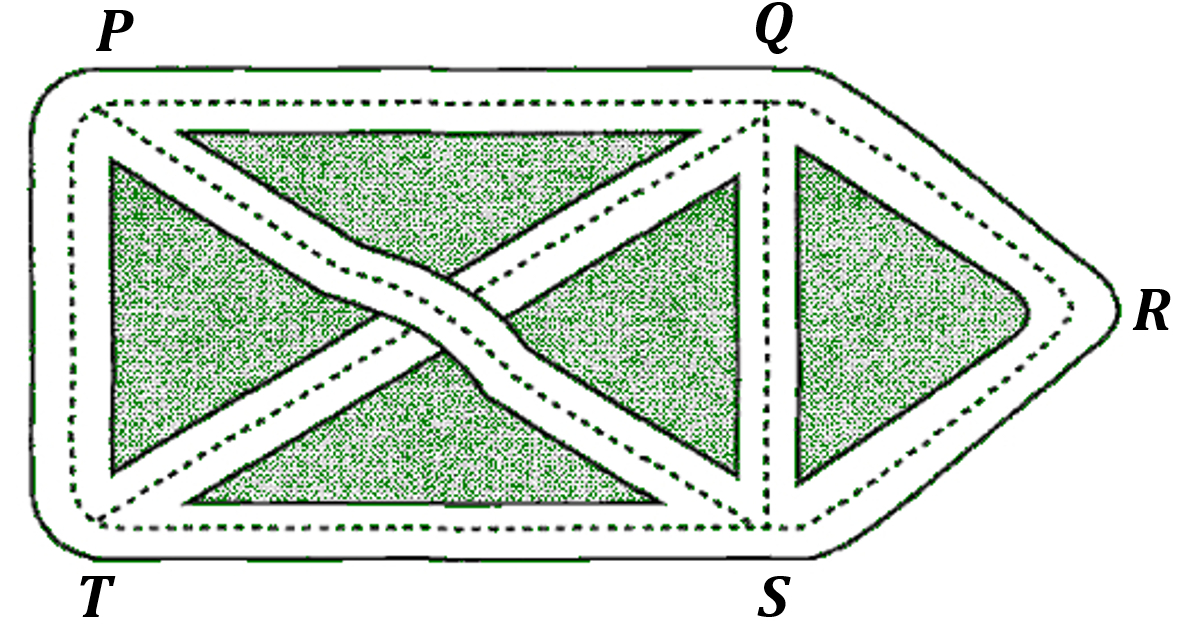
\includegraphics[width=0.8\linewidth]{img/plattegrond.jpg}
	\captionof{figure}{Plattegrond van een park}
	\label{plattegrond}
\end{center}

\begin{center}
	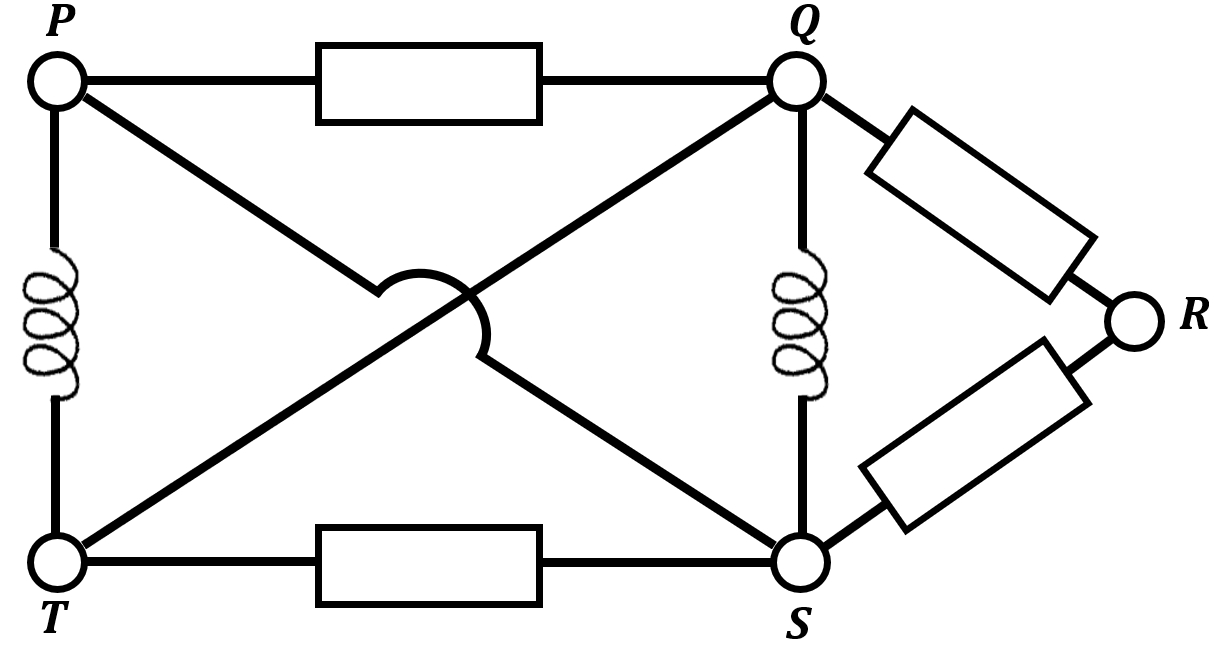
\includegraphics[width=0.85\linewidth]{img/elektrischeschakeling.jpg}
	\captionof{figure}{Elektrische schakeling}
	\label{schakeling}
\end{center}

Het valt onmiddellijk op dat beide eenzelfde structuur hebben. We kunnen deze structuur schematisch voorstellen zoals in figuur \ref{abstraherenmetgraaf}. Deze schematische voorstelling noemen we een {\it graaf}. Wanneer je uitgaat van een formele definitie van het begrip graaf, is het niet helemaal correct om te zeggen dat dit een graaf `is'. Vergelijk met het bekende `Ceci n'est pas une pipe': de voorstelling uit figuur \ref{abstraherenmetgraaf} is een representatie van de graaf, maar het `is' niet die graaf. Voor wat wij hier beogen met deze loep, kiezen wij bewust niet voor zo'n formele aanpak.

\begin{center}
	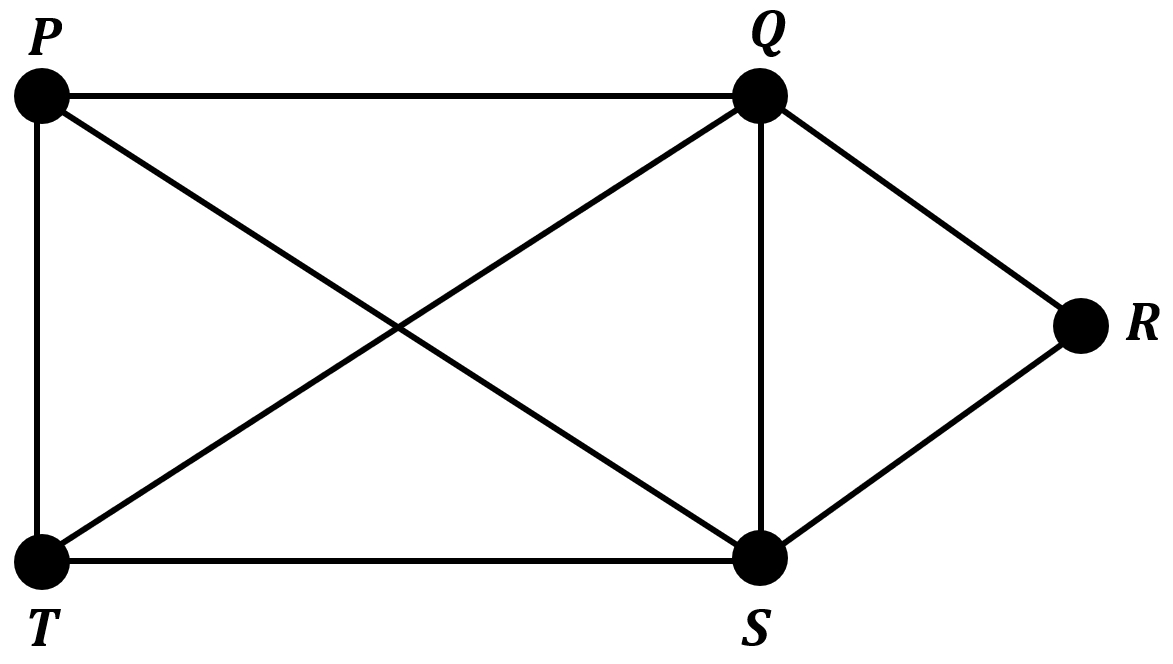
\includegraphics[width=0.8\linewidth]{img/graafabstract.jpg}
	\captionof{figure}{Een graaf bij de plattegrond en de schakeling}
	\label{abstraherenmetgraaf}
\end{center}


Bij een graaf laten we de context, met vaak overbodige info, weg en dat verheldert en vereenvoudigt de situatie. Bovendien: wanneer we een probleem op een graaf kunnen oplossen, kunnen we die oplossing ineens gebruiken voor de verschillende contexten waarin deze graaf voorkomt. 

We bekijken hieronder enkele van de vele contexten en problemen die worden gemodelleerd met grafen.

\textbf{Routes en netwerken}

Een gekend voorbeeld van de kracht van abstractie is dat van een metroplan. De ligging van routes en haltes wordt hierbij niet geografisch correct getekend, ook de afstanden tussen de stations niet. Enkel wat relevant is voor de gebruikers van het plan wordt getoond: de manier waarop de stations onderling verbonden zijn. Zo wordt het voor reizigers eenvoudiger om een route uit te stippelen van het ene station naar het andere. Abstractie zorgt hier voor verduidelijking. 
\begin{center}
	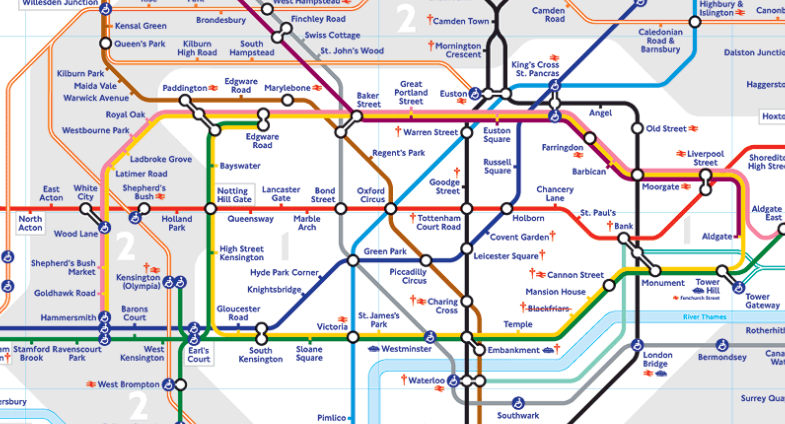
\includegraphics[width=\linewidth]{img/metro.jpg}
	\captionof{figure}{Een stuk van het metroplan van Londen}
	\label{metro}
\end{center}
In andere contexten kan het net handig zijn om afstanden tussen plaatsen te vermelden. Dat is bijvoorbeeld het geval voor verplaatsingen met de auto of met de fiets. Dan willen we soms net de kortste weg tussen twee plaatsen kennen. Dit principe wordt gebruikt bij routeplanners, maar ook bij het plannen van routes voor pakjesdiensten, voor vuilnisophaaldiensten$\ldots$

Het voorbeeld hieronder (figuur \ref{jakoetië}) vonden we bij ResearchGate in een onderzoek naar de optimalisatie van de transportkosten voor landbouwers in Jakoetië (Rusland). Op deze graaf zijn een aantal plaatsen aangeduid (genummerd van 1 tot 12) en hun verbindingswegen. De getallen bij de verbindingswegen zijn een maat voor de transportkosten op die verbindingswegen. Deze maten (of algemener: gewichten) zijn afhankelijk van de aard van de weg, de afstanden, rijtijden$\ldots$
\begin{center}
	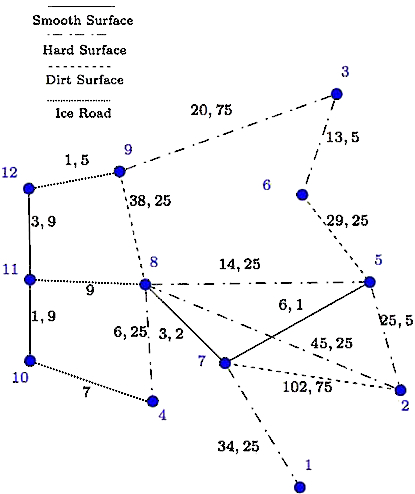
\includegraphics[width=\linewidth]{img/jakoetie.jpg}
	\captionof{figure}{Schematische voorstelling van een wegennet in Jakoetië}
	\label{jakoetië}
\end{center}
Voor een landbouwer die, om leveringen te doen, veel moet rijden tussen zijn velden en klanten is het interessant om de transportkosten bij een route langsheen deze plaatsen te minimaliseren.

Ook online sociale netwerken kunnen worden gemodelleerd met grafen. Een persoon in zo'n netwerk wordt schematisch weergegeven door een  knooppunt. Als twee mensen bevriend zijn, worden `hun' punten verbonden met een boogje.\\ Sociale media apps zoals Facebook, stellen vaak mogelijke vrienden aan je voor. Het suggereren van die potentiële vrienden gebeurt op basis van het aantal vrienden dat je gemeenschappelijk hebt met de kandidaten. Het zoeken van te suggereren vrienden komt dus neer op het zoeken van knooppunten met zoveel mogelijk gemeenschappelijke verbindingen in een graaf.

\columnbreak

\textbf{Chemische verbindingen}

Een molecule bestaat uit een aantal atomen die door chemische verbindingen worden samengehouden. 


Een voorbeeld van zo'n molecule is methaan ($\rm{CH}_4$), het voornaamste bestanddeel van aardgas, dat bestaat uit een koolstofatoom (C) die gebonden zijn aan vier waterstofatomen (H). Schematisch wordt methaan voorgesteld als in figuur \ref{methaan}.
\begin{center}
	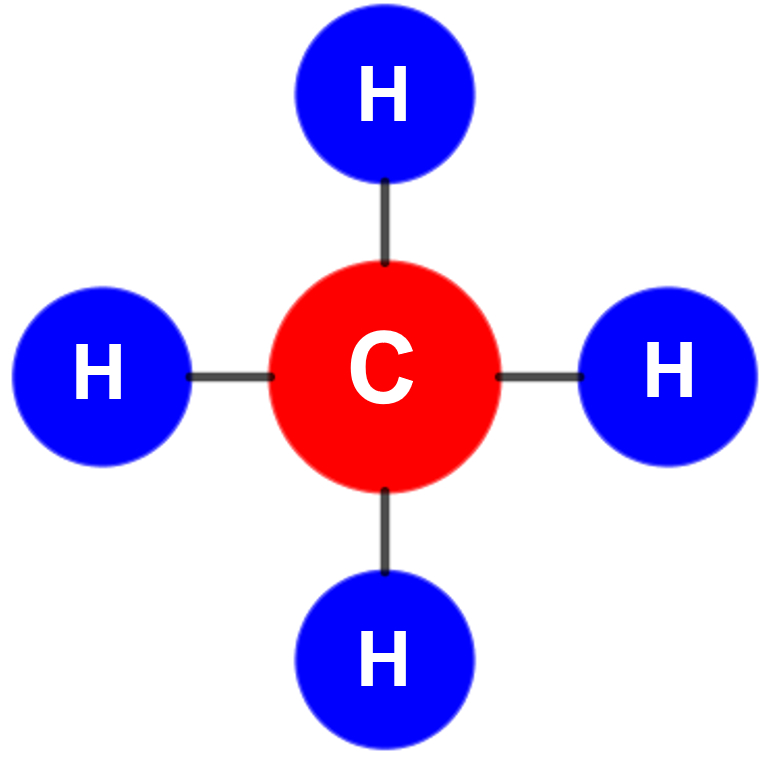
\includegraphics[width=0.4\linewidth]{img/methaan.jpg}
	\captionof{figure}{Schematische voorstelling van methaan}
	\label{methaan}
\end{center}
Deze schematische voorstelling als een graaf vertelt ons niets over de ruimtelijke configuratie van de atomen (de atomen van het methaanmolecule bevinden zich op de hoekpunten van een tetraëder). Wel kunnen we met de voorstelling als graaf onderzoeken hoeveel isomeren er zijn. Isomeren zijn moleculen met een andere structuur, maar met dezelfde chemische formule.
De molecule pentaan bijvoorbeeld, met formule $\rm{C}_5\rm{H}_{12}$, bestaat uit vijf koolstofatomen en twaalf waterstofatomen. Er zijn drie isomeren, zoals getoond in figuur \ref{isomeren}
\begin{center}
	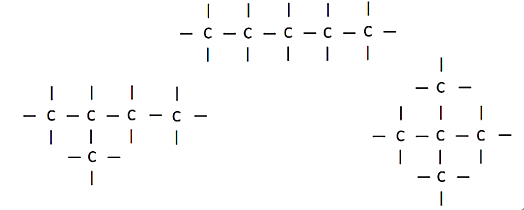
\includegraphics[width=\linewidth]{img/isomeren.jpg}
	\captionof{figure}{De drie isomeren van pentaan}
	\label{isomeren}
\end{center}
Je kunt zelf eenvoudig nagaan dat er juist één molecule is met formule $\rm{C}_3\rm{H}_{8}$ (propaan) en dat er twee zijn met formule $\rm{C}_4\rm{H}_{10}$ (butaan).




\textbf{De drie nutsvoorzieningen}

Een bekende wiskundige puzzel is die van de drie nutsvoorzieningen.
\vspace{-0.5cm}
\begin{quote}
	Drie buren willen hun huizen via leidingen verbinden met de nutsvoorzieningen water, elektriciteit en gas. Ze  willen de negen leidingen zó leggen dat ze in één vlak liggen en dat ze mekaar niet snijden. Is dit mogelijk?
\end{quote}
\vspace{-0.5cm}
Als je het antwoord eerst zelf wilt zoeken, moet je hier het lezen even onderbreken.

In figuur \ref{nutsvoorzieningen} zijn al acht leidingen gelegd, maar huis 1 heeft nog geen elektriciteit. Een variant van het probleem is dan `Kun je deze elektriciteitsleiding leggen zonder de andere leidingen te snijden?'
\begin{center}
	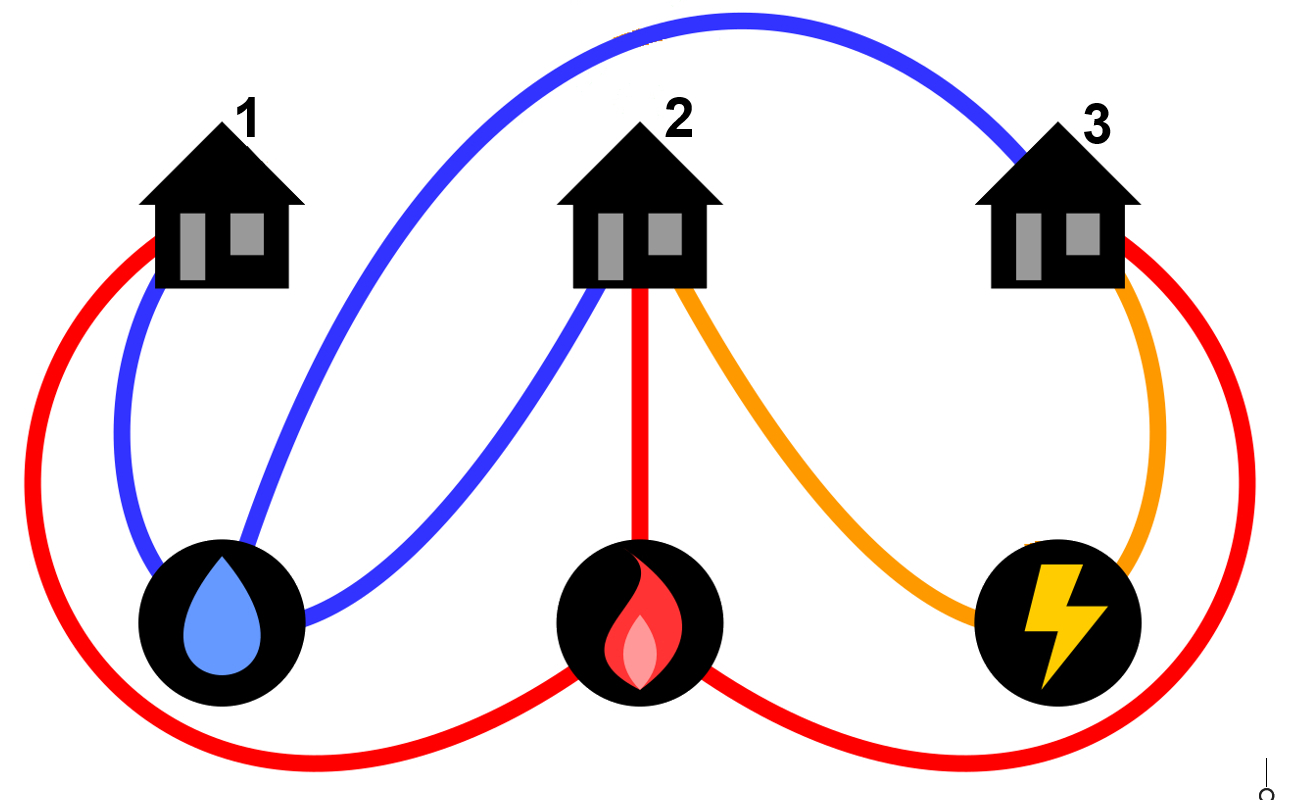
\includegraphics[width=0.8\linewidth]{img/nutsvoorzieningen.jpg}
	\captionof{figure}{Het probleem van de drie nutsvoorzieningen.}
	\label{nutsvoorzieningen}
\end{center}
Om een oplossing te zoeken met zo weinig mogelijk snijden, kun je de huizen en de voorzieningen tekenen in een zeshoek zoals in figuur \ref{nut1}.
\begin{center}
	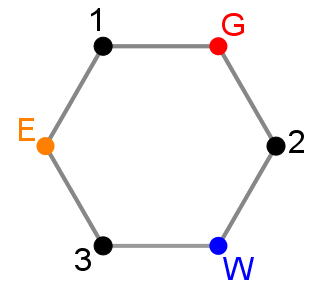
\includegraphics[width=0.4\linewidth]{img/nut1.jpg}
	\captionof{figure}{De huizen en de nutsvoorzieningen in een zeshoek}
	\label{nut1}
\end{center}

Dan moeten nog de verbindingen 1-W, 2-E en 3-G worden getekend. Binnen de zeshoek kan maar één van deze diagonalen worden getekend zonder de andere te snijden. In figuur \ref{nut2} hebben we zo de aansluiting van huis 1 met de watervoorziening getekend.
\begin{center}
	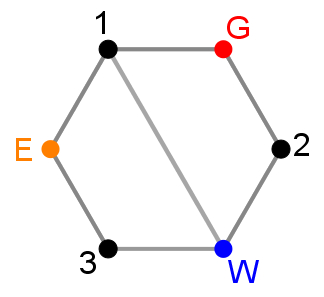
\includegraphics[width=0.4\linewidth]{img/nut2.jpg}
	\captionof{figure}{Binnen de zeshoek kan geen tweede ontbrekende leiding worden getekend}
	\label{nut2}
\end{center}
 
\end{multicols}

\begin{figure}[H]
\centering
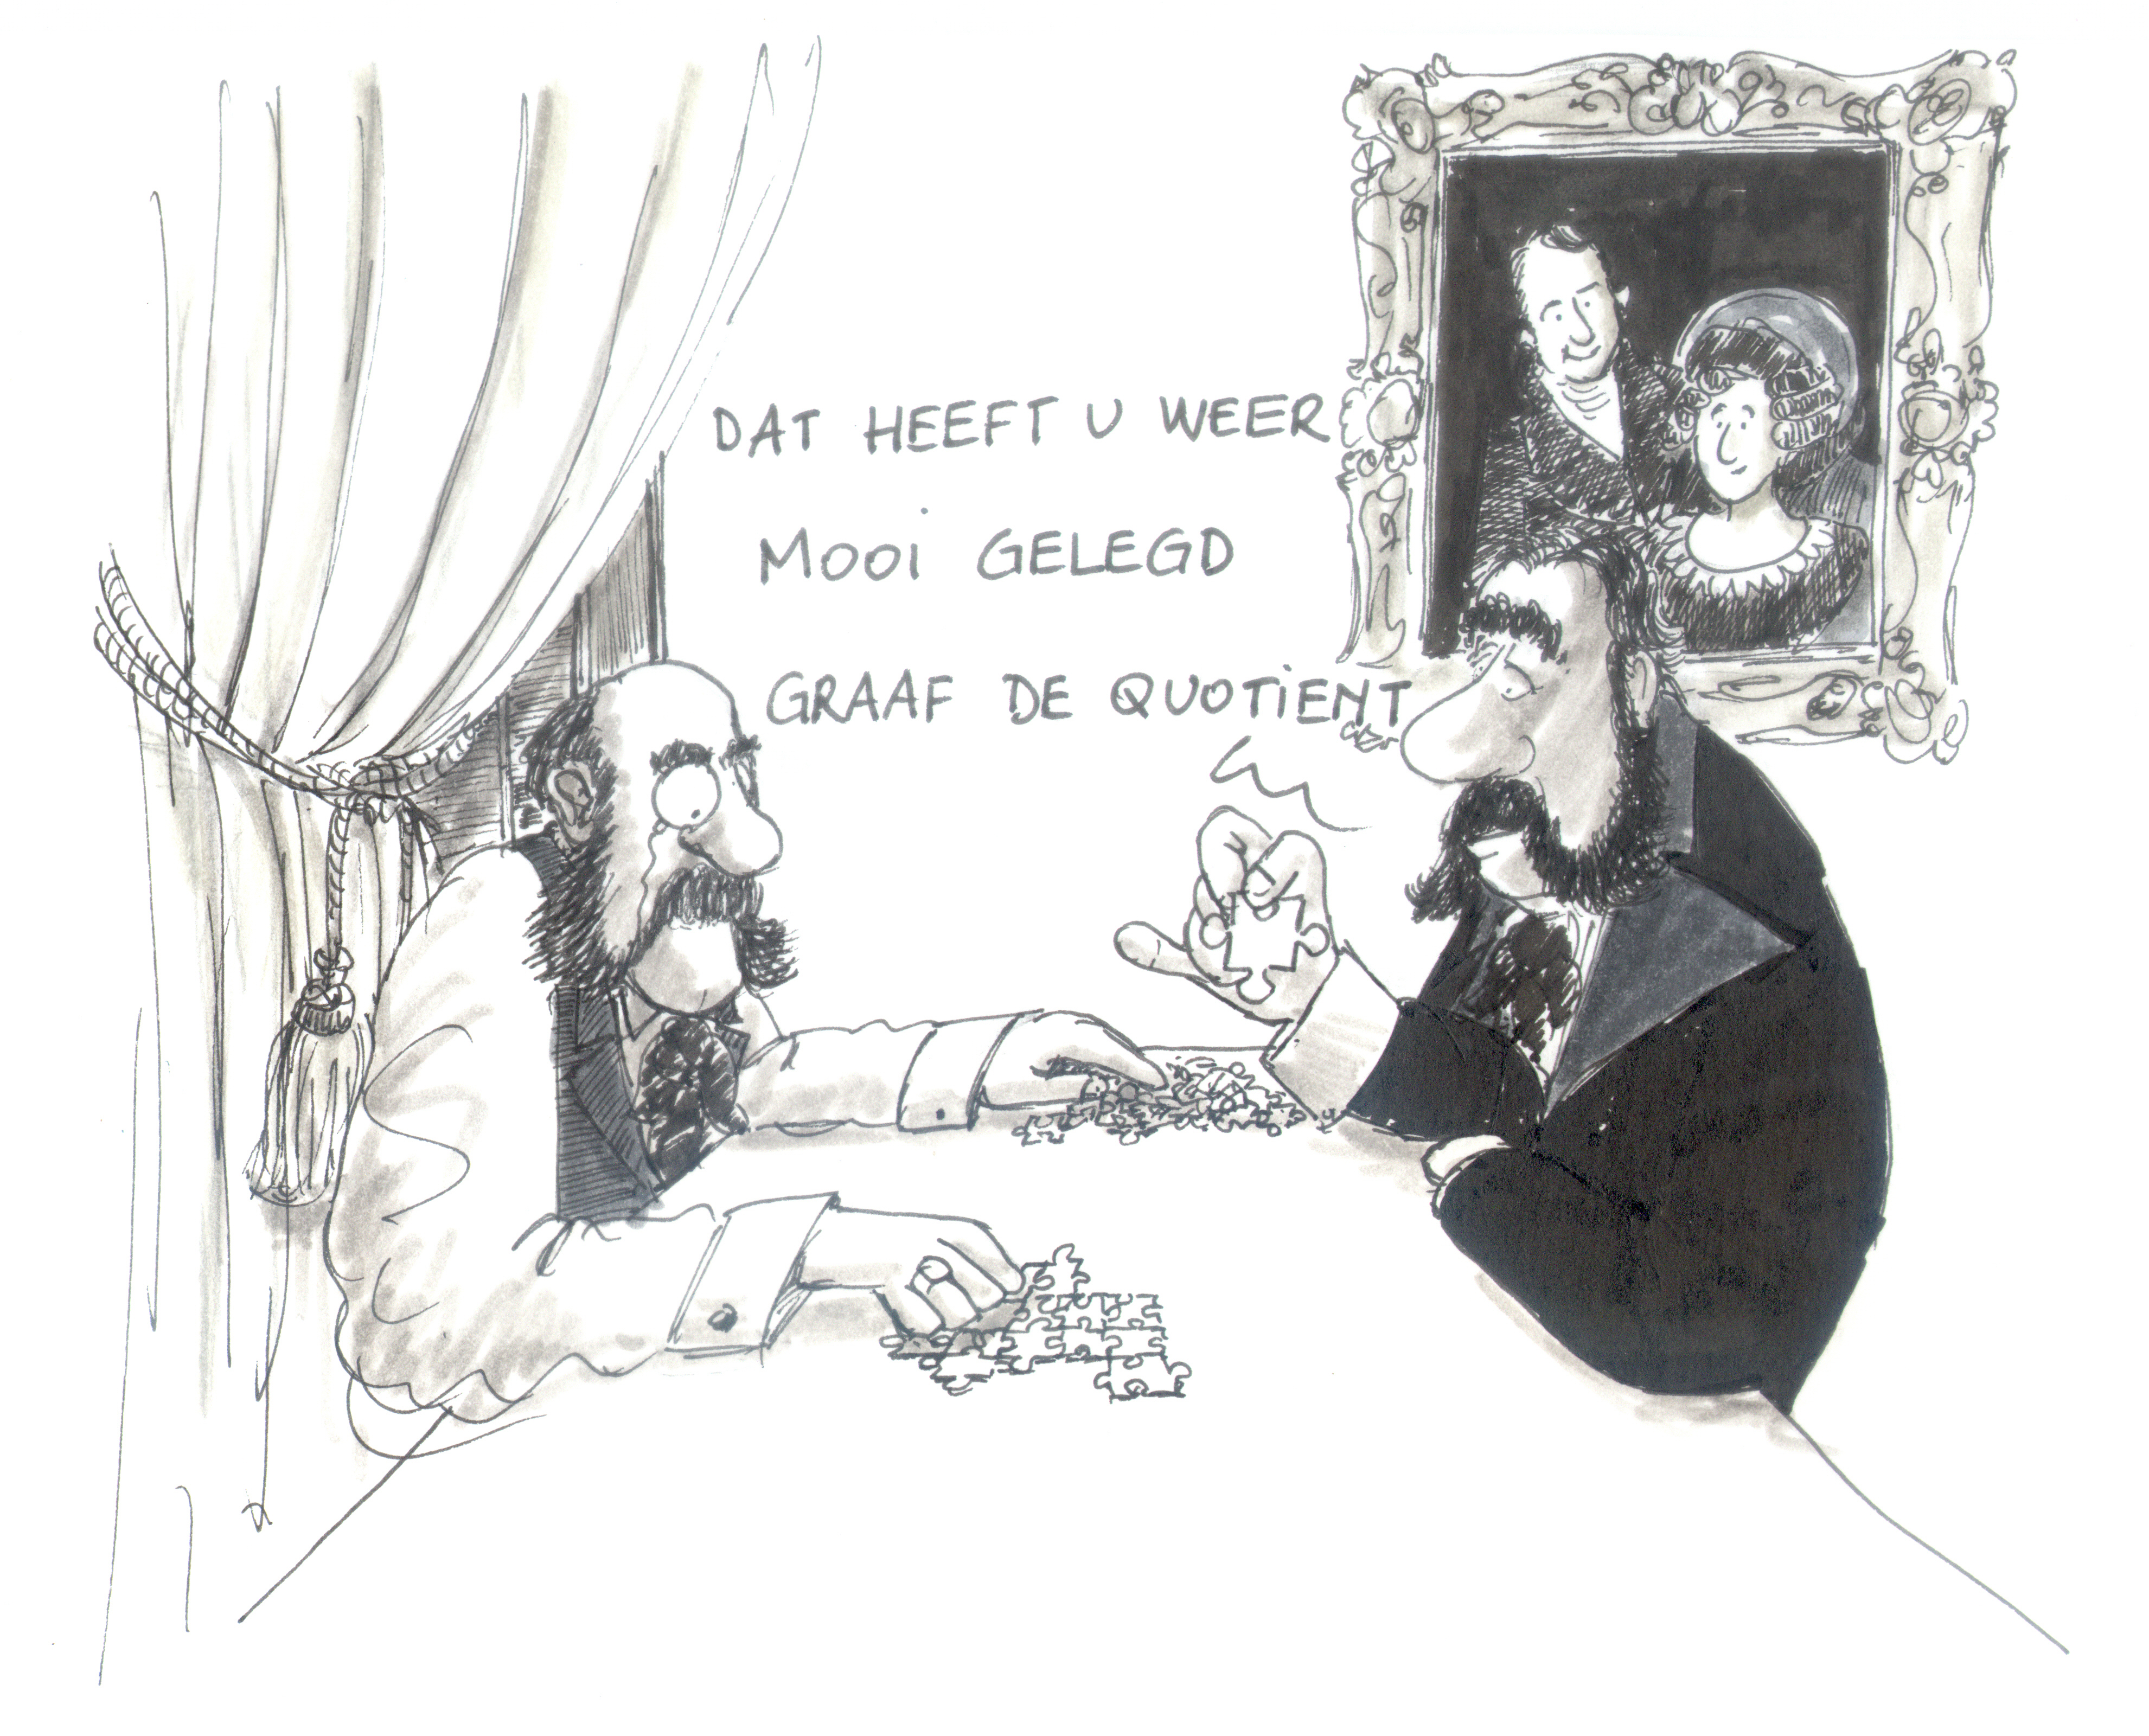
\includegraphics[width=0.8\linewidth]{img/puzzelen.jpg}
\end{figure} 

\begin{multicols}{2} 

Buiten de zeshoek kan nog één verbinding worden getekend zonder de andere leidingen te snijden, bijvoorbeeld met een boog tussen huis 2 en de elektriciteit (zie figuur \ref{nut3}).

\begin{center}
	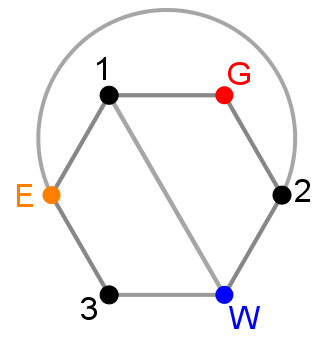
\includegraphics[width=0.4\linewidth]{img/nut3.jpg}
	\captionof{figure}{Een verbinding buiten de zeshoek}
	\label{nut3}
\end{center}
Wanneer je nu de verbinding van huis 3 met de gasvoorziening moet tekenen, dan kun je niet anders dan één van de andere verbindingen snijden. Het probleem van de drie nutsvoorzieningen is niet oplosbaar in een vlak, maar je kunt het wél oplossen op een torus (denk daar maar eens over na). De foto uit figuur \ref{mok} illustreert dit op een originele manier.
\begin{center}
	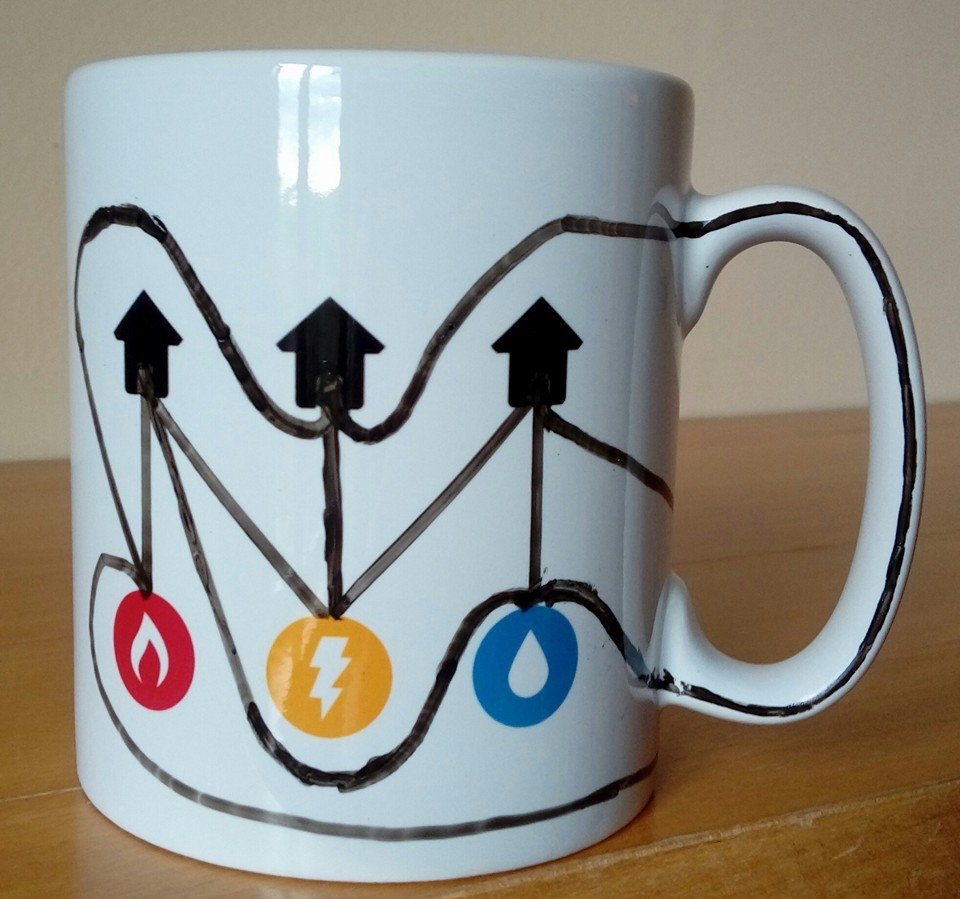
\includegraphics[width=0.5\linewidth]{img/mok.jpg}
	\captionof{figure}{De drie nutsvoorzieningen opgelost}
	\label{mok}
\end{center}

Het probleem van de drie nutsvoorzieningen is vooral interessant omdat het binnen de wiskunde geleid heeft tot allerhande uitdagende veralgemeningen, maar ook omwille van een aantal praktische toepassingen. Zo is het bijvoorbeeld bij het vervaardigen van printplaten voor elektronische componenten (zie figuur \ref{printplaat}) belangrijk dat de geleidende sporen mekaar niet snijden omdat dit zou leiden tot ongewenst elektrisch contact.
\begin{center}
	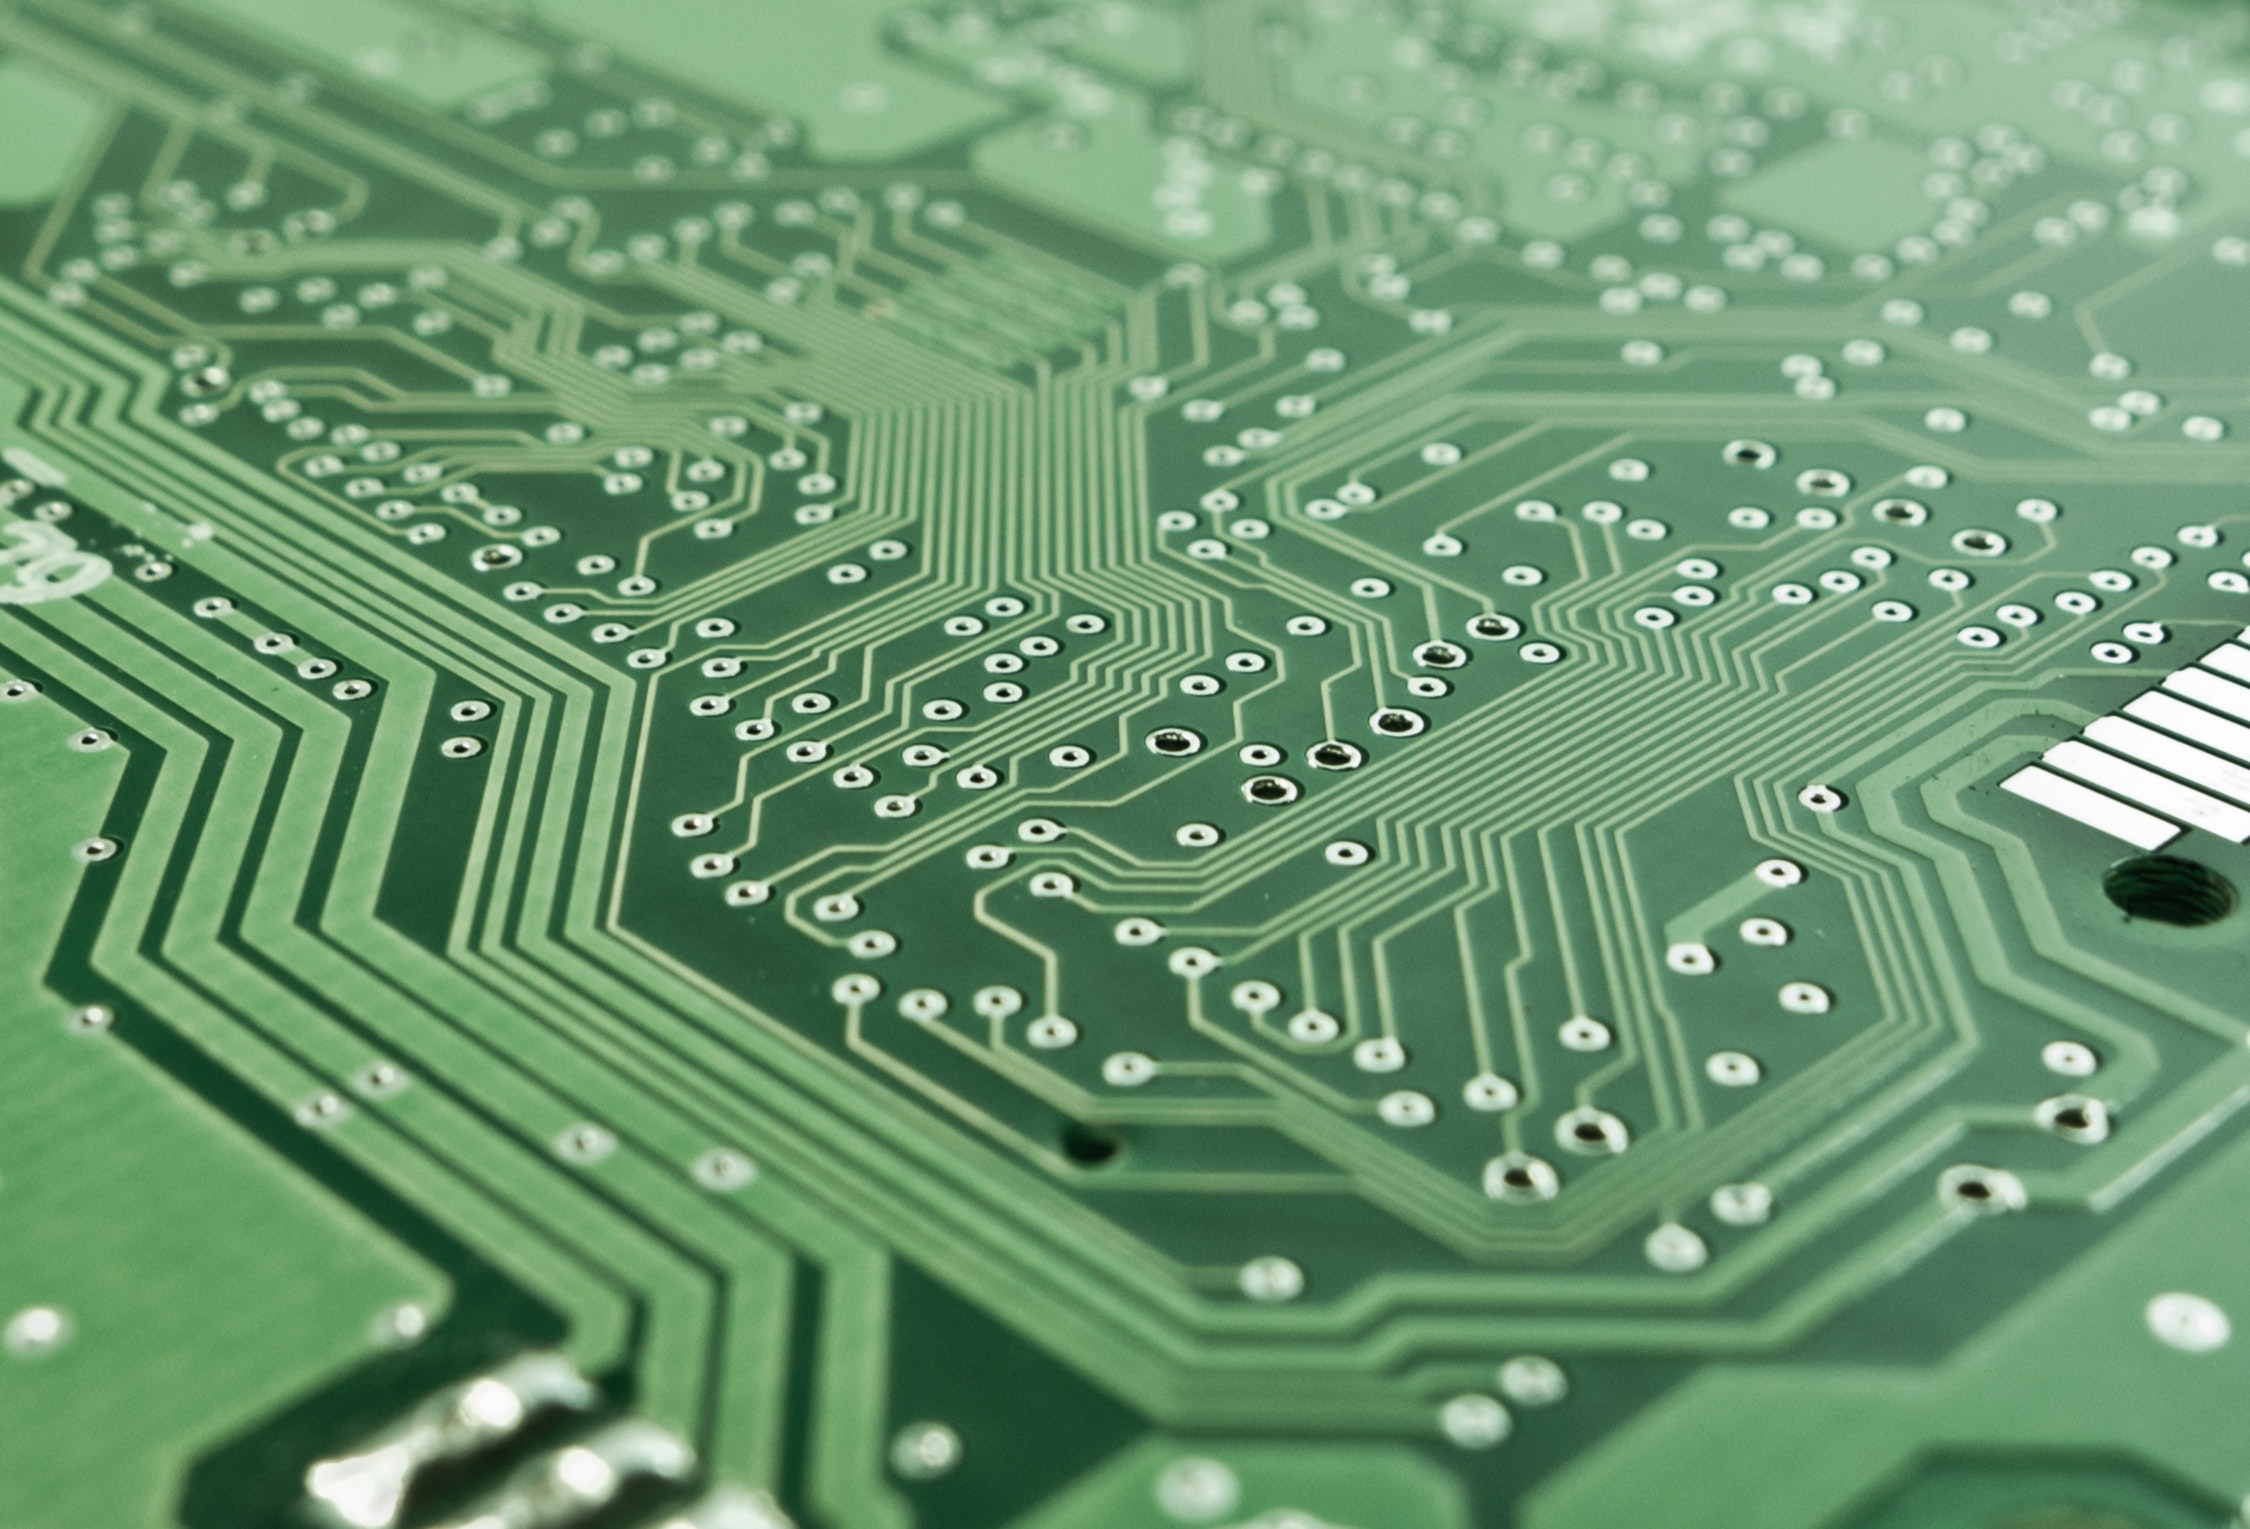
\includegraphics[width=0.7\linewidth]{img/printplaat.jpg}
	\captionof{figure}{De sporen op een printplaat}
	\label{printplaat}
\end{center}


\section{Eerste begrippen over grafen}

Een graaf bestaat uit punten die wel of niet met elkaar verbonden zijn. De punten noemen we \emph{knopen}. In sommige teksten heten ze \emph{toppen}. De Engelse naam is \emph{vertices}, meervoud van \emph{vertex}. De verbindingslijnen noemen wij \emph{bogen}. Je komt ook de naam \emph{kanten} tegen. In het Engels zijn het \emph{edges}.

Merk op dat grafentheorie geen meetkunde is. De plaats van de knopen in het vlak en de vorm en lengte van de bogen hebben helemaal geen belang. De twee tekeningen van figuur \ref{grafen1} stellen dezelfde graaf voor. Het enige wat telt, is welke knopen tot de graaf behoren en welke knopen met welke knopen verbonden zijn door een boog.

\begin{center}
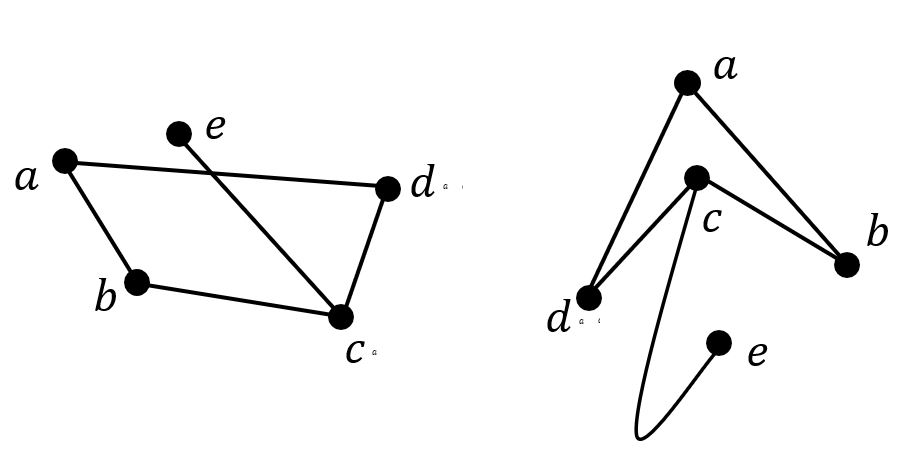
\includegraphics[width=0.65\linewidth]{img/grafen1.jpg}
\captionof{figure}{Twee keer dezelfde graaf}
\label{grafen1}
\end{center}

Een graaf zoals hierboven beschreven wordt soms ook een gewone graaf genoemd. Er bestaan immers ook grafen waarbij er meer dan één boog tussen twee knopen mogelijk is (\emph{multigrafen}), grafen waarbij de bogen voorzien zijn van pijltjes (\emph{gerichte grafen}) en grafen waarbij de bogen voorzien zijn van getallen met de betekenis van bijvoorbeeld afstanden of kostprijzen (\emph{gewogen grafen}). Als we een van deze speciale soorten grafen bedoelen, zullen we het steeds vermelden, zo niet gaat het over gewone grafen.

In sommige boeken wordt een meer formele taal gebruikt om de begrippen te definiëren. Bijvoorbeeld: een graaf $G$ is een geordend tweetal $(V, E)$ waarbij $V$ een verzameling is waarvan we de elementen knopen noemen en $E$ een antireflexieve, symmetrische relatie in $V$. De elementen van $E$ noemen we bogen. Voor wat wij met grafentheorie willen doen, vinden we deze formele verwoording geen meerwaarde.


\subsection{Redeneren met graden van knopen}

In de volgende werktekst wordt een eenvoudig begrip ingevoerd, de graad van een knoop in een graaf. Hiermee kan al meteen geredeneerd worden.

\end{multicols}

\beginwerktekst{De graad van een knoop}

De \emph{graad} van een knoop $a$ in een graaf is het aantal bogen dat in deze knoop toekomt (of: uit deze knoop vertrekt; tenzij bij een gerichte graaf is dit hetzelfde). De knopen die rechtstreeks door een boog verbonden zijn met een knoop $a$ noemen we de \emph{buren} van $a$. De graad van een knoop in een (gewone) graaf is dus het aantal buren van deze knoop. In de figuur hieronder heeft $e$ graad 1; $a$, $b$ en $d$ hebben graad 2; $c$ heeft graad 3. 

\begin{center}
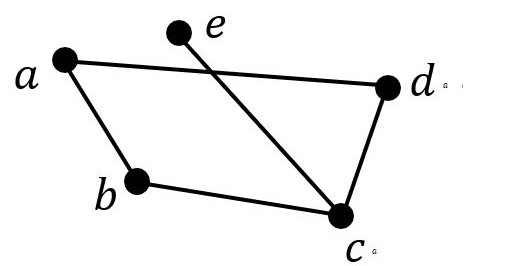
\includegraphics[width=0.22\linewidth]{img/grafengraden.jpg}
\end{center}

\begin{nummering}

\item Hoeveel buren kan een knoop maximaal hebben in een graaf van 250 knopen?

\emph{249}

\item Hoeveel bogen zijn mogelijk in een graaf van 5 knopen? En in een graaf van 10 knopen? En in een graaf van 250 knopen?

\emph{Maximaal 10; 45; 31125 bogen}

\item Teken een graaf. Tel de graden van alle knopen op. Tel ook het aantal bogen. Wat is het verband? Geldt dit altijd? Leg uit.

\emph{De som van de graden is tweemaal het aantal bogen. Bv. in de figuren hieronder: som van de graden: 16, 20; aantal bogen: 8, 10.}

\begin{center}
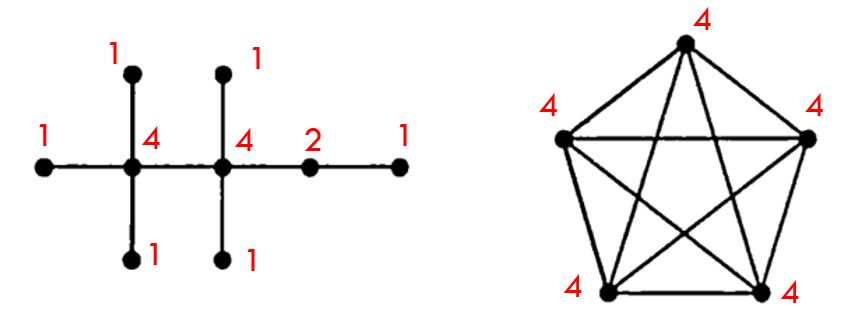
\includegraphics[width=0.55\linewidth]{img/gradensom.JPG}
\end{center}

\emph{Bewijs: bij het optellen van de graden, tel je elke boog twee keer (bij de graad van beide knopen die de boog verbindt).}

\item{Wat kun je zeggen over het aantal knopen met oneven graad in een graaf? Bewijs dit.}

\emph{Een even aantal.} 

\emph{Bewijs: de som van alle graden is even (want tweemaal het aantal bogen). Dus: de som van de oneven graden plus de som van de even graden is even. De som van de oneven graden moet dus even zijn. Dit betekent dat het aantal oneven graden even moet zijn.} 

\emph{Voor sommige leerlingen is dit duidelijker in formulevorm. Noteer de graad van een knoop $a$ met $\deg(a)$, met $\deg$ van degree. Noem $q$ het aantal bogen van de graaf. Noem $a_1$, $a_2$, \dots $a_m$ de knopen met oneven graad en $b_1$, $b_2$, \dots, $b_k$ de knopen met even graad. Dan geldt wegens vraag 3:}
$$\deg(a_1)+\deg(a_2)+\dots +\deg(a_m)+\deg(b_1)+\deg(b_2)+\dots+\deg(b_k)=2q.$$
\emph{Dus is}
$$\deg(a_1)+\deg(a_2)+\dots +\deg(a_m)=2q-(\deg(b_1)+\deg(b_2)+\dots+\deg(b_k))$$
\emph{een verschil van twee even getallen en dus even.}

\end{nummering}

\eindewerktekst

\newpage
\beginwerktekst{Vrienden op feestjes}

De mensen die aanwezig zijn op een feestje, kunnen we voorstellen door knopen van een graaf. Mensen die met elkaar bevriend zijn, verbinden we met een boog. Om dit zo te kunnen voorstellen, gaan we er wel van uit dat twee mensen ofwel bevriend zijn ofwel niet en niet iets tussenin. In de wiskunde houdt men het graag eenvoudig. We nemen ook aan dat niemand bevriend is met zichzelf en dat vriendschap altijd wederzijds is. Je kunt bijvoorbeeld denken aan aanvaarde vriendschap op Facebook.

\begin{nummering}

\item Vertaal naar een eigenschap over grafen: op elk feestje waar minstens twee mensen aanwezig zijn, zijn er steeds (minstens) twee mensen  die juist evenveel vrienden hebben. Bewijs dat.

\emph{Vertaald in grafentheorie betekent dit dat er in een graaf met minstens twee knopen, steeds twee knopen zijn die dezelfde graad hebben.}

\emph{Bewijs: veronderstel dat er $n$ knopen zijn. De hoogst mogelijke graad is $n-1$ (dan is die knoop met alle andere knopen verbonden). Veronderstel dat er geen knopen zijn met gelijke graad. Dan zijn de graden: $0, 1, 2,\dots, n-1$. Dit is immers de enige manier om aan alle knopen verschillende graden toe te kennen. De knoop met graad $0$ is niet met andere knopen verbonden terwijl de knoop met graad $n-1$  met alle andere knopen verbonden is. Dit kan niet. Deze tegenspraak betekent dat de veronderstelling fout was; er zijn dus wel knopen die gelijke graden hebben.}

\item Teken, indien mogelijk, de graaf van een feestje van zes mensen waarvan juist twee met evenveel vrienden. Kun je nog zelf kiezen hoeveel vrienden deze twee hebben, of ligt dat vast?

\emph{Er zijn maar twee mogelijkheden (die je natuurlijk op verschillende manieren kunt voorstellen door de knopen te verplaatsen):}

\begin{multicols}{2}

\begin{center}
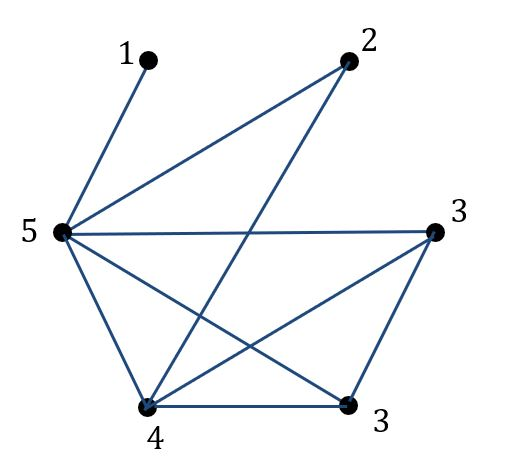
\includegraphics[width=0.75\linewidth]{img/graafvoorbeeld.JPG}
\end{center}

\begin{center}
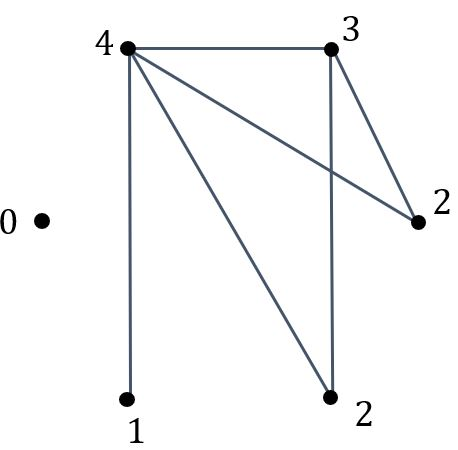
\includegraphics[width=0.65\linewidth]{img/graafvoorbeeld3.JPG}
\end{center}

\end{multicols}

\emph{Merk op dat deze twee grafen `complementair' zijn: in de tweede graaf zijn de knopen verbonden als ze in de eerste niet verbonden zijn en omgekeerd. Dit valt natuurlijk minder op als je de knopen van beide grafen op andere plaatsen tekent. Leerlingen mogen proberen: ze zullen geen andere voorbeelden vinden dan deze twee. Ter informatie voor de lezer: Benjamin e.a. (2015) bewijzen dat er voor elke $n\geq2$ juist twee grafen bestaan met juist twee knopen van gelijke graad en dat die twee grafen `complementair' zijn. Zij bewijzen dit door volledige inductie.}

\item Teken, indien mogelijk, de graaf van een feestje met zes mensen waarbij iedereen ofwel twee ofwel vijf vrienden heeft.

\emph{Bijvoorbeeld:}


\begin{center}
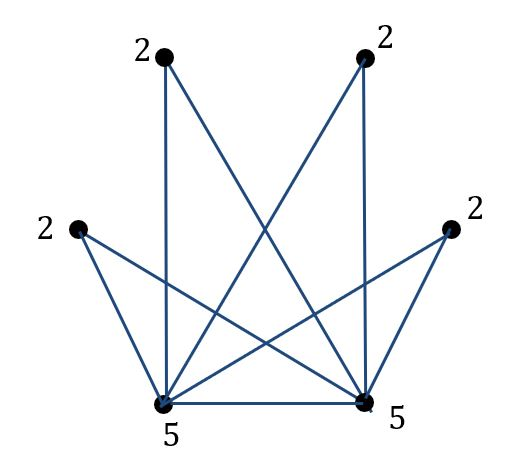
\includegraphics[width=0.35\linewidth]{img/graafvoorbeeld2.JPG}
\end{center}

\item Teken, indien mogelijk, de graaf van een feestje met negen aanwezigen, waarbij iedereen precies met drie andere aanwezigen een Weense wals heeft gedanst.

\emph{De bogen moeten niet altijd vriendschap voorstellen, dit mag ook dansen zijn. Het mag ook disco-swing zijn in plaats van Weense wals. Belangrijk is dat je per twee danst en dat dezelfde eigenschappen gelden als bij vriendschap: je danst niet met jezelf; als $a$ met $b$ danst, dan ook $b$ met $a$...}

\emph{Dit is onmogelijk, want er zouden 9 knopen van graad 3 zijn. Het aantal knopen met een oneven graad kan niet oneven zijn, zie vraag 4 van de vorige activiteit.}

\item Op een feestje met zes mensen zijn er altijd ofwel drie mensen die onderling bevriend zijn, of drie mensen die onderling niet bevriend zijn. Frank Plumpton Ramsey (1903-1930), een Britse filosoof, economist en wiskundige, heeft dit bewezen en veralgemeend tot andere aantallen. Kun je deze eigenschap voor zes mensen ook bewijzen? We geven hieronder enkele tips.

In plaats van de knopen enkel te verbinden in geval van vriendschap, verbinden we de knopen van niet-vrienden ook, maar dan in het grijs in plaats van in het zwart. Het te bewijzen is dan dat er in de graaf ofwel een zwarte driehoek ofwel een grijze driehoek moet bestaan.

\begin{multicols}{3}

\begin{center}
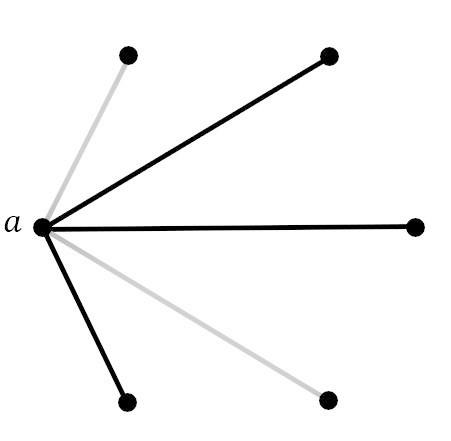
\includegraphics[width=\linewidth]{img/Ramsey1.JPG}

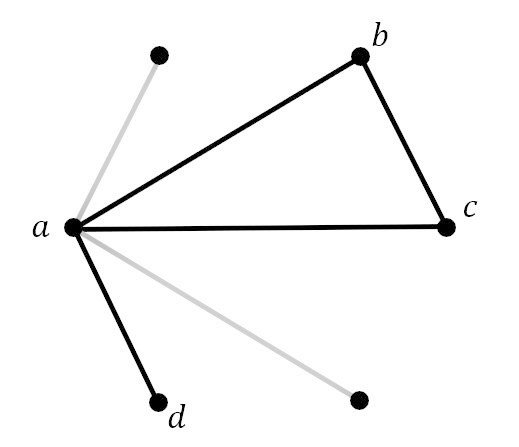
\includegraphics[width=\linewidth]{img/Ramsey2.JPG}

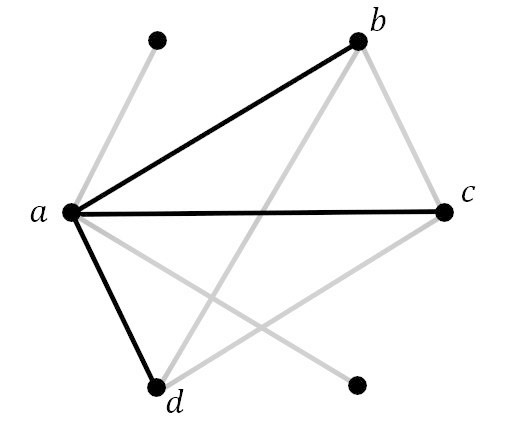
\includegraphics[width=\linewidth]{img/Ramsey3.JPG}

\end{center}

\end{multicols}

Beschouw een knoop $a$. Die is nu verbonden met de vijf andere knopen. Van de vijf bogen die in $a$ samenkomen, zijn er minstens drie in dezelfde kleur. Veronderstel dat het zwart is, maar als het grijs is, gaat het analoog (dan wissel je vanaf hier in de redenering de twee kleuren om). Noem $b$, $c$ en $d$ de knopen die in het zwart verbonden zijn met $a$. Probeer nu verder te redeneren.

\emph{Als twee van de knopen $b$, $c$ en $d$ in het zwart verbonden zijn, bijvoorbeeld $b$ en $c$, dan is het bewijs geleverd want dan hebben we een zwarte driehoek $abc$. Als dat niet zo is, dan zijn deze drie knopen $b$, $c$ en $d$ in het grijs met elkaar verbonden. Dan is het bewijs ook geleverd, want dan hebben we een grijze driehoek $bcd$.}

\item Veronderstel dat Alice en haar lief Brahim op een feestje zijn met drie andere koppels. Bij de begroeting wordt soms wel, soms niet de hand geschud. Niemand schudt hierbij de hand van de eigen partner en niemand schudt meer dan één keer de hand met dezelfde persoon. Na afloop vraagt Alice aan iedereen, ook aan Brahim, hoeveel personen hij of zij de hand geschud heeft. Zij krijgt zeven verschillende antwoorden.

Hoeveel personen heeft Alice de hand geschud?

Hoeveel personen heeft Brahim de hand geschud?

\emph{Het antwoord is telkens 3.}

\emph{Noem Alice en Brahim $a$ en $b$. De andere koppels noemen we $c$ en $d$, $e$ en $f$, $g$ en $h$.} 

\emph{De graden van $b$, $c$, \dots $h$ moeten $0, 1\dots 6$ zijn. Het getal $7$ komt niet voor want niemand schudt de eigen partner de hand. De graad van $b$ kan niet $6$ zijn, want dan zou Brahim met iedereen behalve Alice de hand geschud hebben, en zou graad $0$ niet meer voorkomen onder de graden van $c$, $d$,  \dots $h$.}

\emph{Veronderstel dat $\deg(c)=6$. Dit doet geen afbreuk aan de algemeenheid. We verbinden $c$ dus met alle andere knopen behalve de partner $d$. Dan moet $\deg(d)=0$, want dat is de enige knoop die nog niet verbonden is.}

\emph{De graad van b kan ook niet 5 zijn, want dan zou b iedereen behalve a en d een hand gegeven hebben. De graad 1 zou dan niet voorkomen. Veronderstel dan dat $\deg(e)=5$. Dit doet weer geen afbreuk aan de algemeenheid. We verbinden $e$ dus met de knopen $g$, $h$, $a$ en $b$. Dan moet $\deg(f)=1$ want de andere knopen behalve $d$ hebben al minstens twee buren.}  

\emph{De graad van b kan ook niet 4 zijn. Als dat wel zo was, had hij g en h allebei de hand geschud. Maar dan hebben g en h allebei minstens graad 3 en ontbreekt graad 2. Veronderstel dus dat $\deg(g)=4$. We verbinden $g$ dus met $a$ en $b$. Dan moet $h$ de knoop zijn met graad 2. We zijn klaar en we zien dat $\deg(a)=\deg(b)=3.$}

\begin{multicols}{2}

\begin{center}
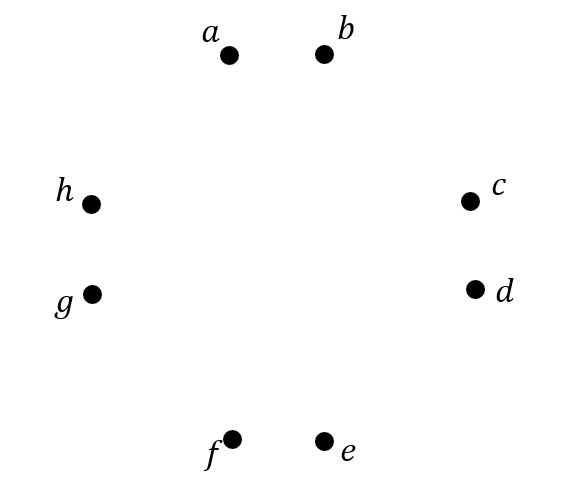
\includegraphics[width=0.8\linewidth]{img/handen1.jpg}

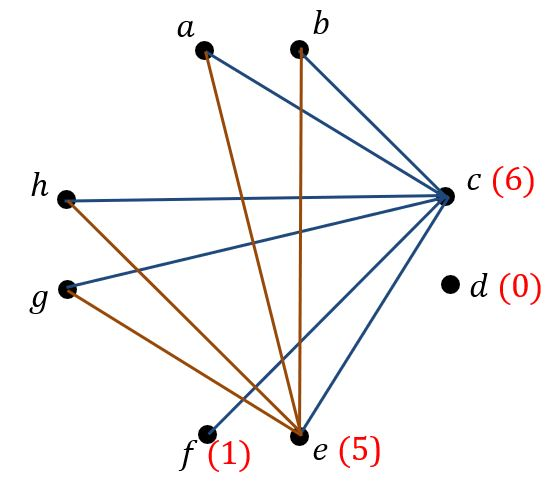
\includegraphics[width=0.8\linewidth]{img/handen3.jpg}

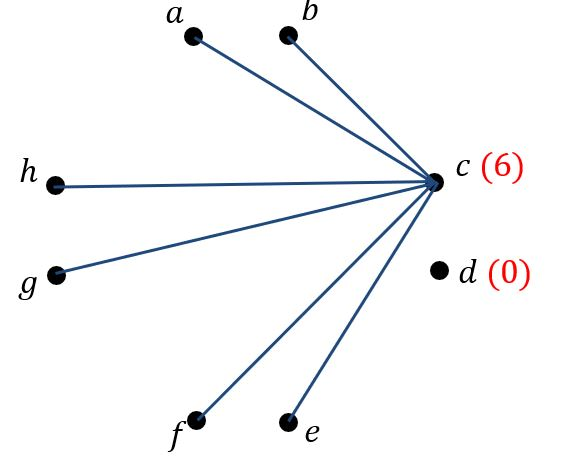
\includegraphics[width=0.8\linewidth]{img/handen2.jpg}

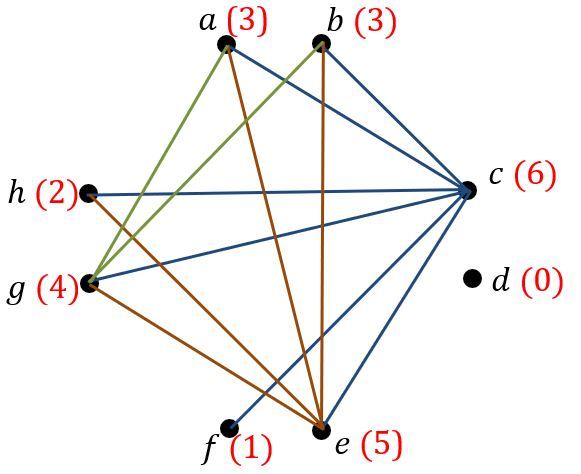
\includegraphics[width=0.8\linewidth]{img/handen4.jpg}

\end{center}

\end{multicols}

\end{nummering}

\eindewerktekst


\begin{multicols}{2}

\subsection{Redeneren met nieuwe definities}

Als je aan de leerlingen een definitie wilt aanbrengen die ze nadien moeten kennen, laat je die niet uit de lucht vallen, maar breng je die aan met voorbeelden en tegenvoorbeelden. Maar het kan ook eens interessant zijn om de leerlingen als oefening een nieuwe definitie te geven die ze moeten interpreteren. Leerlingen moeten zelf voorbeelden en tegenvoorbeelden geven om aan te tonen dat ze de definitie begrijpen. Ze krijgen uitspraken waarvan ze moeten zeggen of ze waar zijn of niet, en uitleggen waarom.

Sommige begrippen (pad, cykel, tweedelingsgraaf, boom...) komen verderop in deze loep nog terug.

\end{multicols}

\beginwerktekst{Samenhangende grafen en bruggen}

Lees de volgende definities. Je hebt ze nodig voor de vragen die erop volgen.

Een \emph{pad} van een knoop $a$ naar een knoop $b$ ($\neq a$) in een graaf $G$ is een opeenvolging van bogen van $G$ waarop je van $a$ naar $b$ kunt wandelen zonder dat je onderweg meer dan één keer langs eenzelfde knoop passeert. In de figuur hieronder is $badcef$ één van de vele paden van de graaf. 

\begin{multicols}{2}

\begin{center}
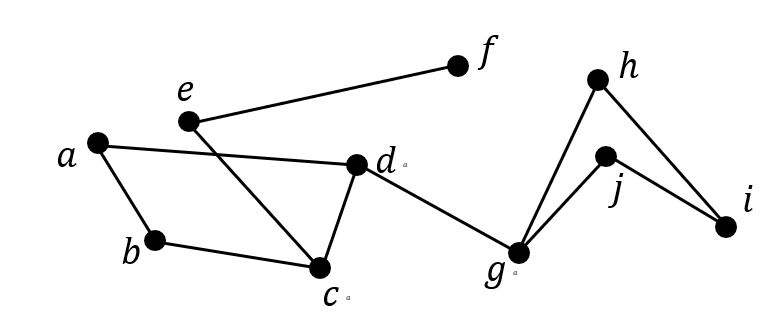
\includegraphics[width=0.8\linewidth]{img/voorbeeldpad.jpg}

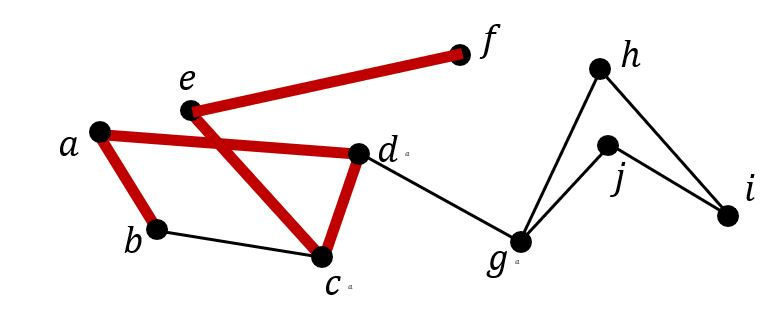
\includegraphics[width=0.8\linewidth]{img/voorbeeldpad2.jpg}
\end{center}

\end{multicols}

Een \emph{cykel} is een opeenvolging van bogen van de graaf waarop je van een knoop $a$ naar dezelfde knoop $a$ kunt wandelen zonder dat je onderweg meer dan één keer langs eenzelfde knoop passeert. In de vorige figuur zijn $abcda$ en $ghijg$ twee cykels.

Een graaf is \emph{samenhangend} als tussen elk paar knopen een pad in de graaf aanwezig is. De graaf van de tien knopen $a, \dots,  j$ in de vorige figuur is samenhangend.

Een boog in een graaf is een \emph{brug} als de graaf samenhangend is maar als je die boog wegneemt niet meer.

\begin{nummering}

\item Geef alle bruggen van de graaf van de figuur in het begin van deze werktekst.

\emph{De boog $dg$, maar ook $ce$ en $ef$. Dat zijn ze.}

\item Waar of niet? Leg uit of geef een tegenvoorbeeld.

\subitem Als een boog in een graaf G een brug is, dan maakt deze boog geen deel uit van een cykel.

\subitem Als een boog in een graaf geen deel uitmaakt van een cykel, dan is dat een brug.

\emph{De eerste uitspraak is waar. Bewijs. Veronderstel dat boog $ab$ een brug is maar wel deel uitmaakt van een cykel $abcde...fa$. Als je de boog $ab$ wegneemt, zou de graaf niet meer samenhangend mogen zijn (definitie van brug). Maar: je kunt  een pad vinden van $a$ naar $b$, namelijk $af...edcb$. De knopen die verbonden waren zonder via de boog $ab$ te passeren, zijn dit nog steeds. En de knopen die verbonden waren via $ab$, zijn nu verbonden via de omweg $af...edcb$. De graaf is dus nog steeds samenhangend. Tegenspraak.}


\begin{center}
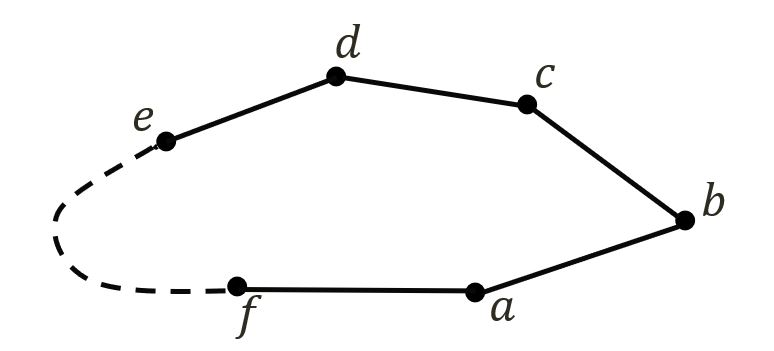
\includegraphics[width=0.35\linewidth]{img/brugbewijs.JPG}

\end{center}

\emph{De tweede uitspraak is ook waar. Bewijs. Veronderstel dat boog $ab$ geen deel uitmaakt van een cykel maar geen brug is. Als je $ab$ wegneemt is de graaf samenhangend. Je kunt dus van $a$ naar $b$ wandelen langs een pad, bv. (om de vorige figuur te recycleren) $af...edcb$. Maar dan is $af...edcba$ een cykel van de graaf, en $ab$ maakt er deel van uit. Tegenspraak.}

\end{nummering}

\eindewerktekst

\beginwerktekst{Tweedelingsgrafen of bipartiete grafen}

Een \emph{tweedelingsgraaf} (of een \emph{bipartiete graaf}) is een graaf waarvan je de knopen in twee groepen kunt verdelen zodanig dat elke boog van de graaf een knoop van de ene groep verbindt met een knoop van de andere groep. Anders gezegd: er mogen geen bogen zijn tussen knopen van dezelfde groep. Belangrijk in deze definitie is het woordje `kunt': als je de knopen in twee groepen verdeelt en je ziet een boog binnen een zelfde groep, kan het zijn dat je de verdeling in groepen moet herzien...

\begin{nummering}

\item Teken een tweedelingsgraaf van 7 knopen.

\emph{Bijvoorbeeld:}

\begin{center}
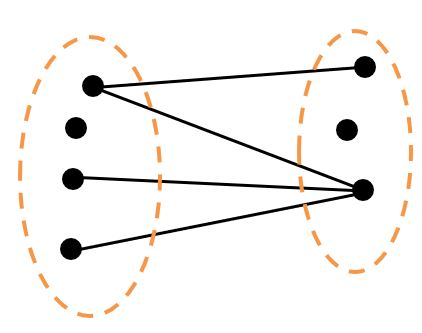
\includegraphics[width=0.25\linewidth]{img/tweedelingsgraaf.jpg}

\end{center}

\emph{Je kunt de twee groepjes van een tweedelingsgraaf aanduiden met kringen zoals in de figuur. Je kunt ook twee kleuren gebruiken om de knopen van de twee groepjes aan te duiden. De graaf hieronder is dezelfde als de vorige, maar anders voorgesteld.}

\begin{center}
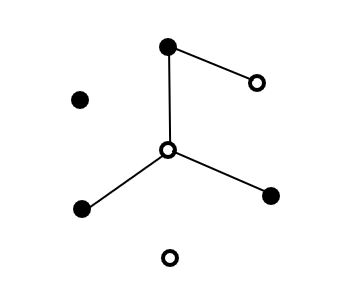
\includegraphics[width=0.25\linewidth]{img/tweedelingsgraaf10.jpg}
\end{center}

\item Zijn de volgende grafen tweedelingsgrafen? Leg uit. 

\begin{multicols}{3}

\begin{center}

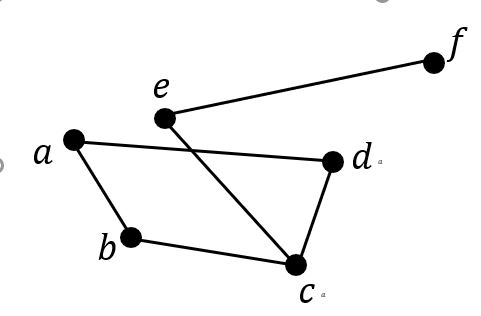
\includegraphics[width=0.9\linewidth]{img/tweedelingsgraaf3.jpg}


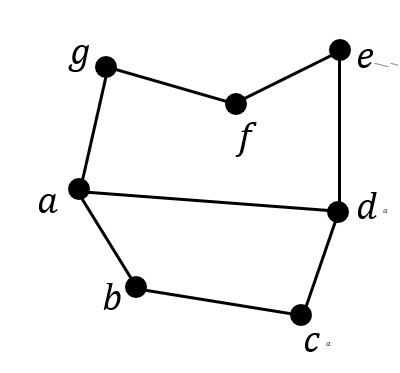
\includegraphics[width=0.8\linewidth]{img/tweedelingsgraaf4.jpg}

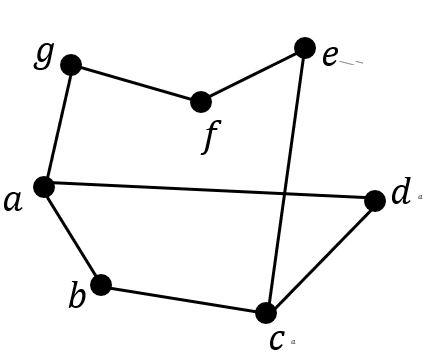
\includegraphics[width=0.8\linewidth]{img/tweedelingsgraaf5.jpg}
\end{center}

\end{multicols}

\emph{De eerste graaf is een tweedelingsgraaf. Je kunt als groepjes $\{a, c, f\}$ en $\{b, d, e\}$ nemen.}

\emph{De tweede graaf is geen tweedelingsgraaf. Als $a$ in één groepje zit, laten we zeggen groep 1, dan moet $g$ in groep 2 zitten, $f$ in groep 1, $e$ in groep 2, $d$ in groep 1 (want knopen die verbonden zijn door een boog mogen niet in hetzelfde groepje zitten). Maar dan is er een boog die $a$ en $d$, knopen van hetzelfde groepje, verbindt, wat niet mag in een tweedelingsgraaf.}

\emph{De derde graaf is wel een tweedelingsgraaf, met groepjes $\{a, c, f\}$ en $\{b, d, e, g\}$.}

\end{nummering}

Een oneven cykel is een cykel met een oneven aantal bogen (en dus ook met een oneven aantal knopen).

\begin{nummering}

\setcounter{enumi}{2}

\item Een bekende stelling zegt:

een graaf $G$ is een tweedelingsgraaf $\Leftrightarrow$ $G$ bevat geen oneven cykel. 

Eén van de twee implicaties is gemakkelijk te bewijzen. Welke?

De andere implicatie is iets moeilijker en zullen we hier niet aantonen.

\emph{De implicatie $\Rightarrow$, namelijk dat een tweedelingsgraaf geen oneven cykel mag hebben, is gemakkelijk te bewijzen. Als je de knopen van een cykel in een tweedelingsgraaf overloopt, moet je die om beurten in één van de twee groepjes kunnen plaatsen. Daarom moet het aantal knopen van die cykel even zijn. De andere implicatie is moeilijker omdat je moet aantonen dat die twee groepen bestaan.}


\end{nummering}

\eindewerktekst

\newpage

\beginwerktekst{Bomen}

Een \emph{boom} is een samenhangende graaf zonder cykels.

\begin{figure}[H]
\centering
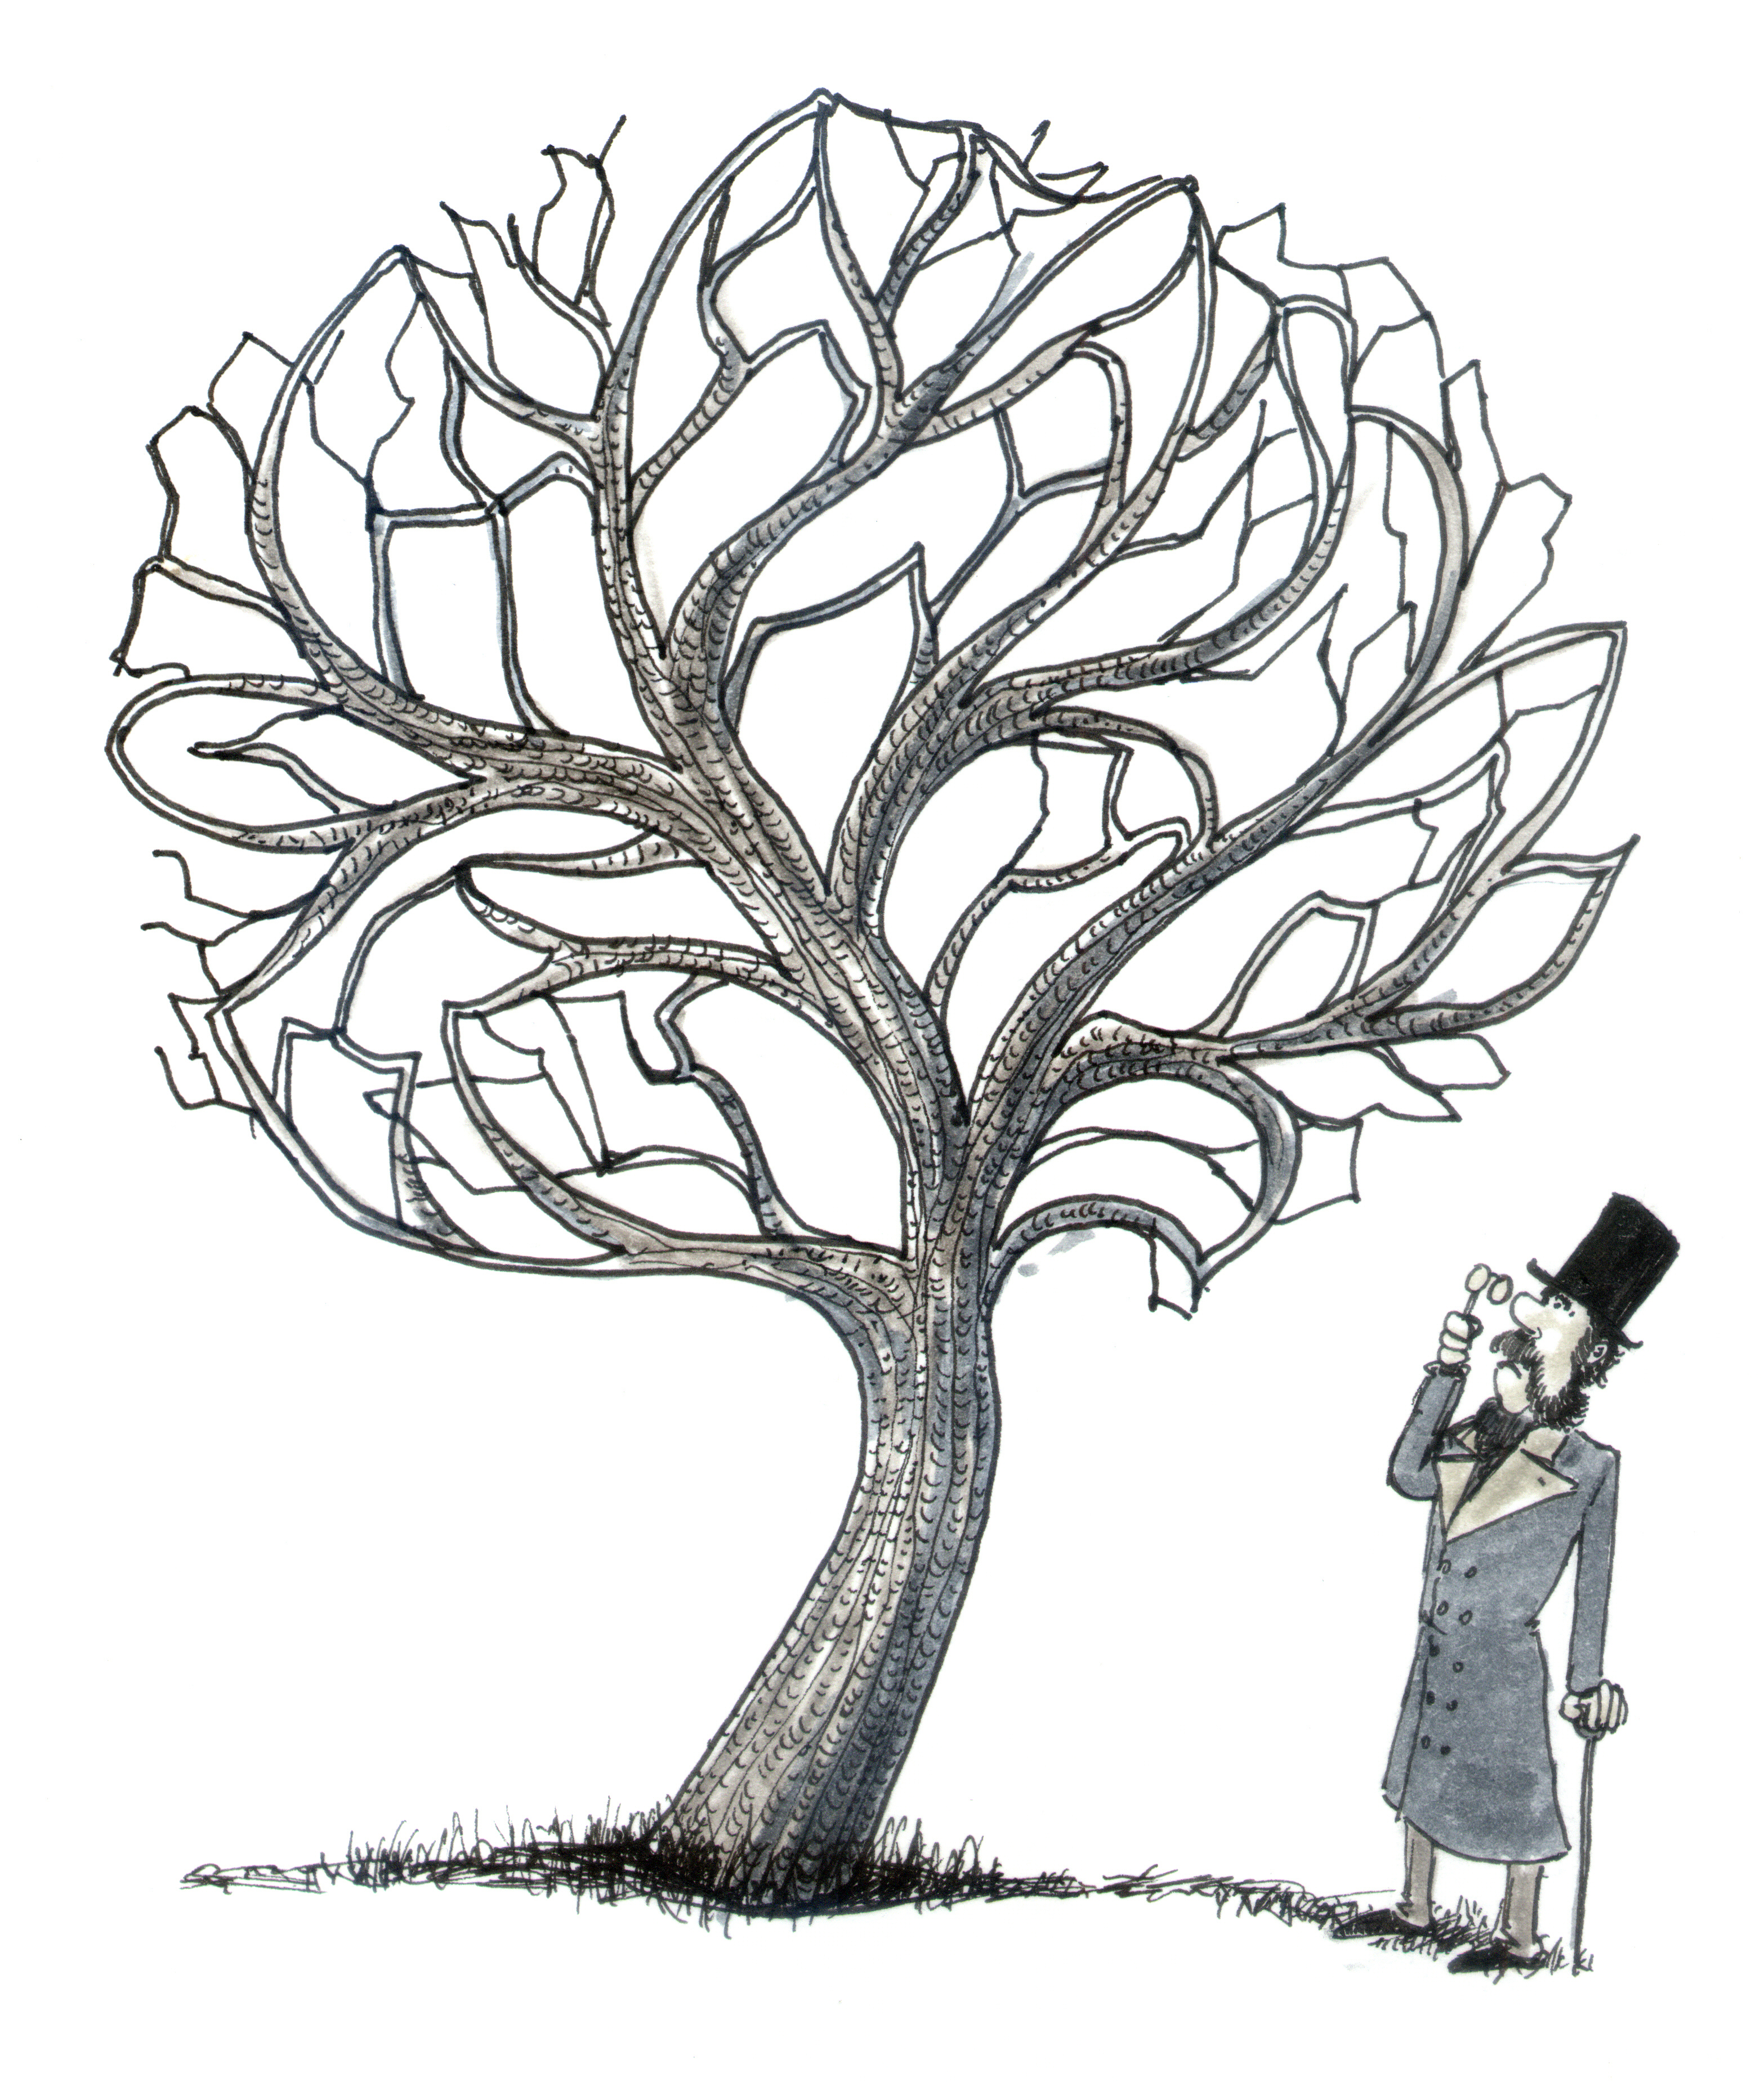
\includegraphics[width=0.7\linewidth]{img/boom.jpg}
\end{figure} 

\begin{nummering}

\item Teken een boom.

\emph{Net als het begrip brug, krijgt een woord uit het dagelijkse leven een wiskundige betekenis. Sommige leerlingen zullen misschien een boom tekenen die er (min of meer) uit ziet als een boom in de natuur, met takken en eventueel ook wortels. Maar bomen in de grafentheorie kunnen er ook heel anders uitzien, als ze maar voldoen aan de definitie. Hieronder zie je drie voorbeelden van bomen.}

\begin{center}
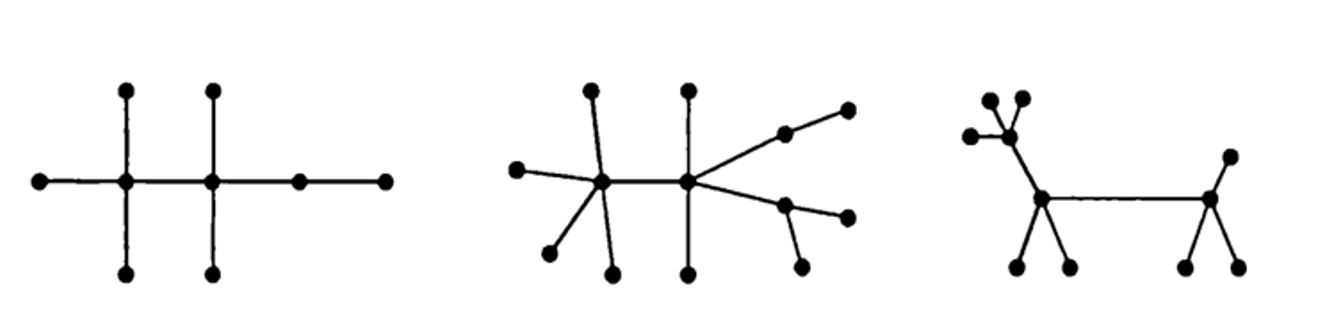
\includegraphics[width=0.8\linewidth]{img/bomen.JPG}
\end{center}

\item Bewijs: in een boom is elk paar knopen verbonden door juist één pad.

\emph{Hier zijn twee zaken te bewijzen: (1) elk paar knopen is verbonden door een pad (minstens één) en (2) er is nooit meer dan één pad tussen dezelfde twee knopen.}

\emph{Omdat een boom samenhangend is, geldt alvast (1).}

\emph{Veronderstel nu dat er in een boom twee verschillende paden zijn tussen een knoop $a$ en een knoop $b$. Dan ontstaat er een cykel (zie figuren hieronder), wat niet kan in een boom.}

\begin{center}
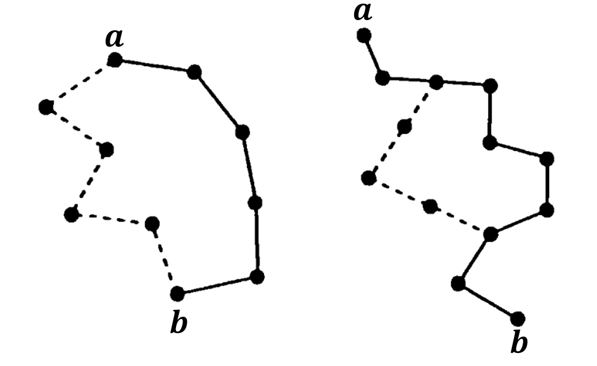
\includegraphics[width=0.45\linewidth]{img/bomen2.JPG}
\end{center}

\end{nummering}

\eindewerktekst

\begin{multicols}{2}

\section{Hamiltongrafen}


In deze paragraaf gaan we dieper in op de zogenaamde hamiltongrafen. We voeren eerst de basisbegrippen in met het spel dat Hamilton bedacht en waaraan de hamiltongrafen hun naam ontlenen. Daarna behandelen we een gekende puzzel waarmee we de kracht van abstractie tonen. Tot slot volgen nog enkele kleine oefeningetjes waarin we voor bepaalde types van grafen onderzoeken of ze hamiltongrafen zijn.

%\subsection{Reis rond de wereld}

In 1857 ontwierp de beroemde Ierse wiskundige Sir William Rowan Hamilton een spel, in het Engels The Icosian Game genoemd. Hierbij moesten de spelers een route vinden langs de ribben van een dodecaëder (zie figuur \ref{dodecaëder}). Voorwaarde was dat die route elk hoekpunt juist één keer aandeed en terugkeerde naar het beginpunt. Het spel werd schematisch voorgesteld in een plat vlak, met een planaire graaf (of een vlakke graaf) d.w.z. een graaf waarvan de bogen mekaar niet snijden buiten de knopen (zie figuren \ref{icosian} en \ref{dodecaplanair}). 

\begin{center}
	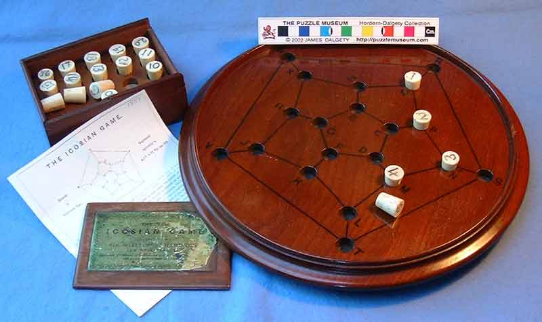
\includegraphics[width=0.8\linewidth]{img/spelhamilton.jpg}
	\captionof{figure}{Een originele versie van The Icosian Game van Sir William Hamilton}
	\label{icosian}
\end{center}

Je verkrijgt deze planaire graaf, ook wel het Schlegeldiagram genoemd, door te kijken naar de dodecaëder vanuit een punt net erbuiten, recht in het midden vóór een zijvlak (regelmatige vijfhoek) en dan te tekenen wat je ziet. Je bekomt zo een centrale projectie vanuit dat oogpunt. In de graaf die hoort bij het spel komen de knopen overeen met de hoekpunten van de dodecaëder en de bogen met de ribben. Een hamiltongraaf was geboren.

Merk op dat het probleem van de drie nutsvoorzieningen dat we in paragraaf 2 bestudeerden neerkomt op nagaan of de graaf die hoort bij het probleem, planair is.

Een \emph{hamiltonpad} in een graaf is een pad dat elke knoop van die graaf juist één keer aandoet. Is dat pad gesloten, dan spreken we van een \emph{hamiltoncykel}. \emph{Hamiltongrafen} zijn grafen die een hamiltoncykel bevatten.


\begin{center}
	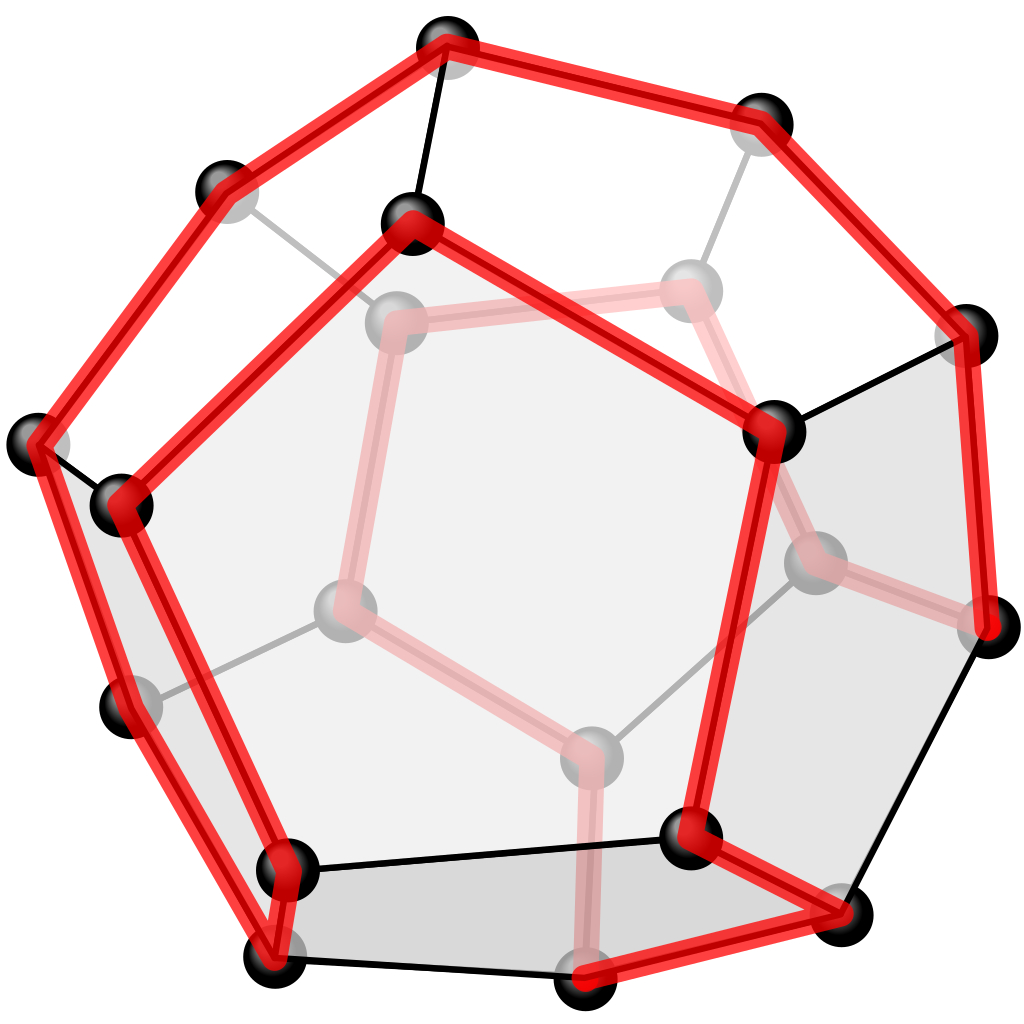
\includegraphics[width=0.45\linewidth]{img/dodecaeder.jpg}
	\captionof{figure}{Een hamiltoncykel op een dodecaëder}
	\label{dodecaëder}
\end{center}

\begin{center}
	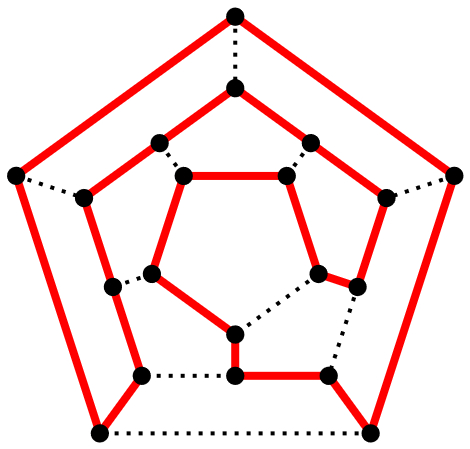
\includegraphics[width=0.5\linewidth]{img/dodecaedergraaf.jpg}
	\captionof{figure}{De schematische voorstelling van de bovenstaande hamiltoncykel in een planaire graaf}
	\label{dodecaplanair}
\end{center}


Hamilton gaf instructies mee met zijn spel en voorbeelden van mogelijke spelvormen met twee spelers. Zo stelde hij een versie voor waarbij een speler de eerste vijf knopen van een hamiltoncykel kiest voor zijn tegenspeler, die dan de cykel moet voltooien. Er werden ook versies van het spel uitgegeven waarbij de knopen grote steden voorstellen, verspreid over heel de wereld.  Doel van het spel was dan een reis rond de wereld te vinden waarbij je elke stad maar één keer bezoekt. In de volgende lesactiviteit spelen we deze vorm. Aan de hand van deze activiteit kun je eventueel de begrippen rond hamiltongrafen introduceren. 

Voorzie genoeg afdrukken van de graaf en zorg dat er kleurpotloden zijn.

\end{multicols}

\beginwerktekst{Een reis rond de wereld met grafen}


In 1857 vond de Ierse wiskundige Sir William Rowan Hamilton het spel `Een reis rond de wereld' uit. Er zijn verschillende versies van dat spel verschenen. Wij spelen hier een vorm met twee spelers.

De letters (alle medeklinkers) bij de knopen in de onderstaande graaf stellen steden voor, verspreid over heel de wereld: Brussel, Canton, Delhi ... Een route zoeken betekent dus een reis rond de wereld maken waarbij je elke stad slechts één keer bezoekt.

De eerste speler moet een pad van vijf opeenvolgende knopen kiezen om te starten. Zijn tegenspeler moet dit pad verder afmaken, ermee rekening houdend dat elke stad juist één keer moet bezocht worden en dat de reis moet eindigen waar ze begonnen is. Zo bijvoorbeeld kan de eerste speler het spel starten met de reeks $BCPNM$. De tweede speler kan de reis dan afmaken op twee manieren: met de route $DFKLTSRQZXWVJHGB$ of via $DFGHXWVJKLTSRQZB$.


\begin{center}
	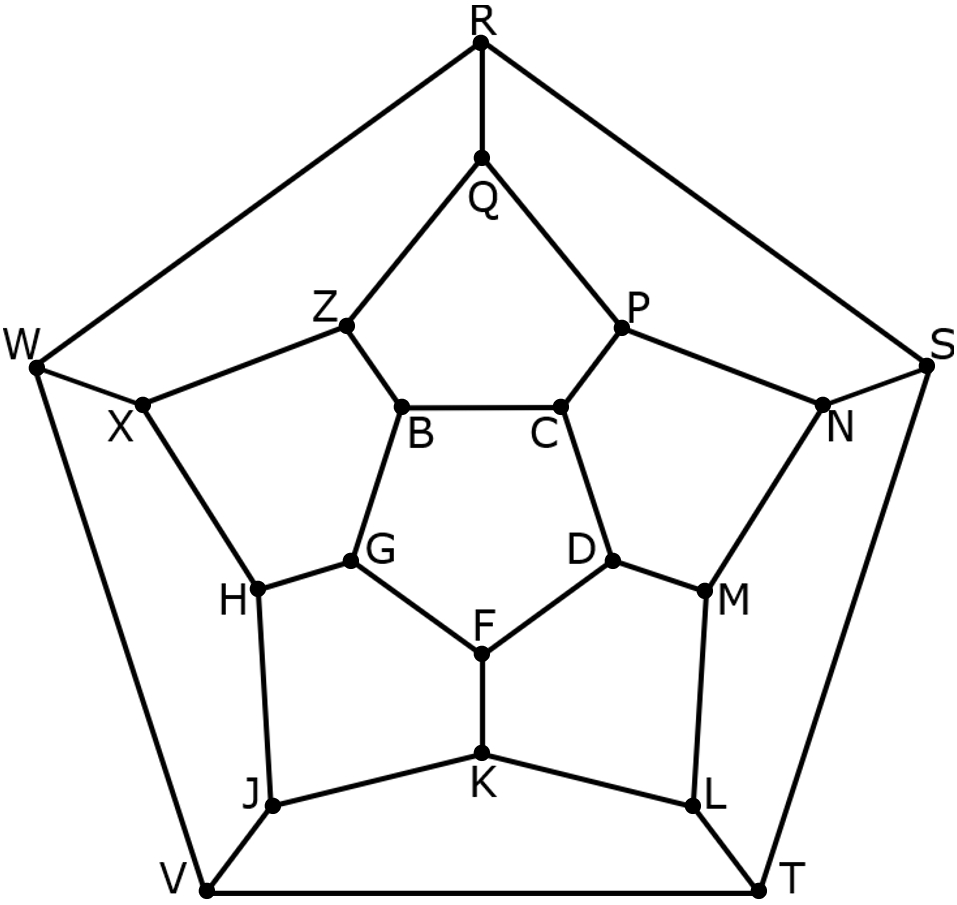
\includegraphics[width=0.5\linewidth]{img/reisronddewereld.jpg}
\end{center}


\begin{nummering}

\item Speel het spel enkele keren. Je kunt met kleur de reisroute aanduiden.
 
\item Hoeveel mogelijke routes zijn er als je reis begint met $JVTSR$?

\emph{Er zijn twee mogelijke routes: $WXZQPNMLKFDCBGHJ$ OF $WXHGFDCBZQPNMLKJ$. Merk op dat na de letter $R$ sowieso de letter $W$ moet komen omdat anders de letter $W$ overgeslagen wordt.}

\item Stel dat het spel gestart werd met de opeenvolging $BCPNM$. Toon aan dat de routes $DFKLTSRQZXWVJHGB$ en $DFGHXWVJKLTSRQZB$ de enige mogelijke routes zijn waarmee de reis kan worden afgemaakt door de details in de argumentatie van hieronder verder aan te vullen. Duid als onderdeel van je bewijs op de graaf elke stap van de redenering aan in een andere kleur.\\ Als je na de eerste deelvragen het gevoel hebt dat je op eigen houtje verder kunt, probeer dat dan zeker!
\begin{enumerate}
	\item Leg uit waarom uit de manier waarop je start volgt dat zeker de opeenvolging $RST$ of $TSR$ moet voorkomen in de reisroute.
	
	\emph{Als $S$ niet tussen $R$ en $T$ staat, kun je $S$ niet meer bereiken omdat je al in $N$ bent geweest. Je moet dus in $S$ aankomen langs $R$ of langs $T$ en uit $S$ vertrekken langs de andere stad.}
	
	\item Leg uit waarom nog door de manier van starten zeker ook $RQZ$ of $ZQR$ moet voorkomen in de reisroute.
	
	\emph{Analoog als hierboven. In $Q$ zijn er drie bogen. Omdat je gestart bent in $P$, mag je daar niet meer naartoe. Je moet dus $Q$ bereiken via $Z$ of via $R$ en er weer weggaan via de andere stad.}
	
	\item Leg uit waarom je nu kunt besluiten dat $XWV$ of $VWX$ een stuk moet zijn van de reisroute.
	
	\emph{$R$ is een gemeenschappelijke knoop van de reeksen uit (a) en (b). Daarom kun je niet meer vanuit $R$ naar $W$ gaan. $W$ is dus nog enkel bereikbaar vanuit $X$ of vanuit $V$. Dus: $W$ moet tussen $X$ en $V$ liggen.}
	
	\item Leg uit waarom door de start van de route ook $FDM$ of $MDF$ in de route moet zitten.
	
	\emph{$D$ is verbonden met $F$, $C$ en $M$. Je kunt zeker niet meer langs $C$ gaan omdat je al in $C$ geweest bent en $C$ geen uiteinde is van een vorige reeks. Daarom kun je niet anders dan $D$ binnen- of buitengaan via $F$ of $M$ en dat betekent dat $D$ tussen $F$ en $M$ moet liggen.}
	
	\item Leg uit waarom we nu uit (d) kunnen concluderen dat $KLT$ of $TLK$ op het reispad moeten liggen.
	
	\emph{Stad $L$ kan niet meer bereikt worden via $M$ want $M$ is gemeenschappelijke knoop bij de startreeks en de reeks uit (d).  De enige mogelijkheid om nog in $L$ te geraken, is dus via $K$ of via $T$. $L$ moet daarom tussen $K$ en $T$ liggen.}
	
	\item Gebruik nu al de vorige bevindingen om te bewijzen dat de twee oplossingen $DFKLTSRQZXWVJHGB$ en $DFGHXWVJKLTSRQZB$ de enige oplossingen zijn.
	
	\emph{Vanuit $M$ moet je de verbinding maken met een reeks van hierboven. Dat kan enkel maar met $MDF$. De reis bevat dus zeker de reeks $BCPNMDF$. Vanuit $F$ sluit je ofwel aan bij $KLT$ ofwel bij $G$. 
		\begin{itemize}
			\item In het eerste geval, moet je verder met $TSR$ en verkrijg je dus de reeks $BCPNMDFKLTSR$. Omdat $R$ een gemeenschappelijke knoop is, kan het niet anders dan dat je reis verder gaat langs $RQZ$ en dan $XWV$ (vanuit $Z$ is er maar één knoop waar je naartoe kunt). Dan zijn de enige knopen die je nog niet hebt bezocht $JHG$. Vanuit $G$ kom je zo terug in $B$ en ben je de wereld rond gereisd. 
			\item In het tweede geval moet je vanuit $G$ naar $H$ en daarna is de enige optie om de route verder te zetten via $XWVJKLTSRQZB$. Anders zou je vanuit $H$ naar $J$ gaan, maar dan moet je kiezen tussen twee `uiteinden' van een groepje nl. $K$ of $V$. Welke keuze je ook maakt: het andere uiteinde blijft altijd een los eindje waar het spoor dood loopt zodat je niet meer kunt eindigen in $B$.
		\end{itemize} }
		
\end{enumerate}

\end{nummering}

\begin{figure}[H]
\centering
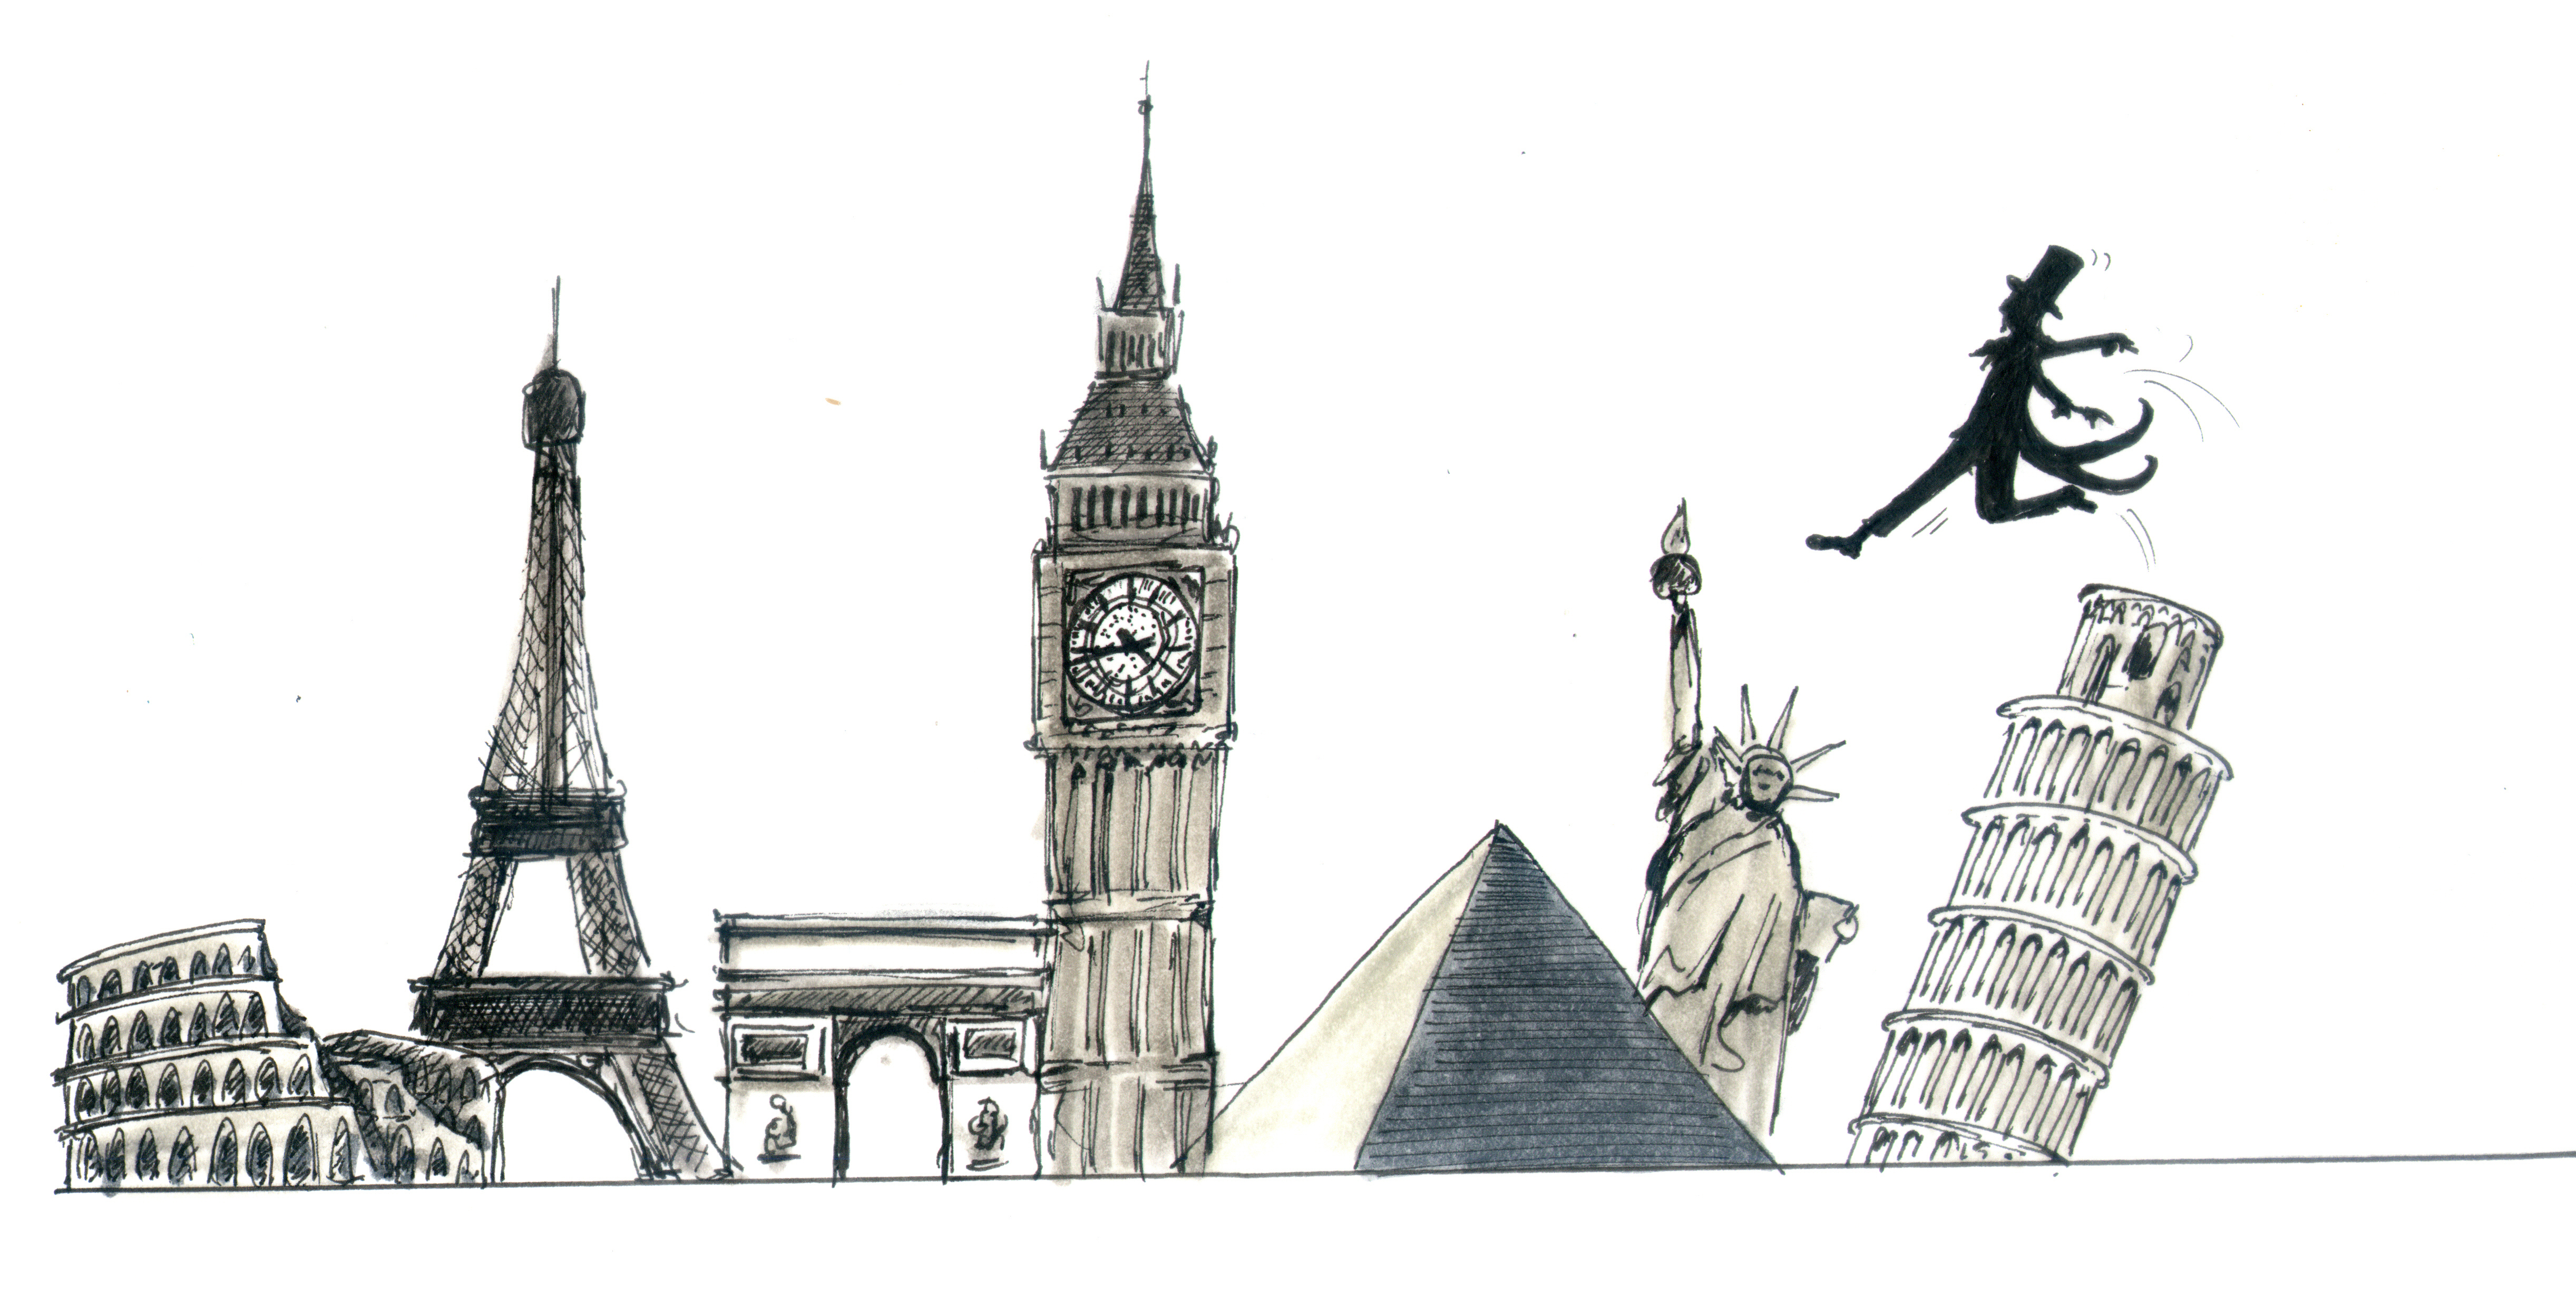
\includegraphics[width=0.95\linewidth]{img/citytrip.jpg}
\end{figure} 
\eindewerktekst

\begin{multicols}{2}


%\subsection{Paardenrondgangen}

Een ander typisch voorbeeld bij hamiltongrafen is de paardenrondgang (Engels: knight's tour). Dit is een mooie puzzel die op het eerste gezicht complex lijkt (en dat in bepaalde versies ook wel degelijk is), maar die je met de juiste graaf soms heel eenvoudig kunt oplossen. In de onderstaande lesactiviteit lossen we een voorbeeld van zo'n paardenrondgangpuzzel op en bestuderen we ook enkele andere versies.

\end{multicols}

\beginwerktekst{De paardenrondgang}



 Bij het schaakspel mag een paard steeds twee velden horizontaal in combinatie met één veld verticaal bewegen of het mag twee velden verticaal met één veld horizontaal springen. Het beweegt dus steeds volgens een L-vorm.
  
 Stel dat het paard nu niet beweegt op een gewoon schaakbord maar op een klein kruisvormig schaakbord zoals in de figuur hieronder. Op de figuur zijn ook de zetten getekend die mogelijk zijn als het paard start op veld 1.

\begin{center}
	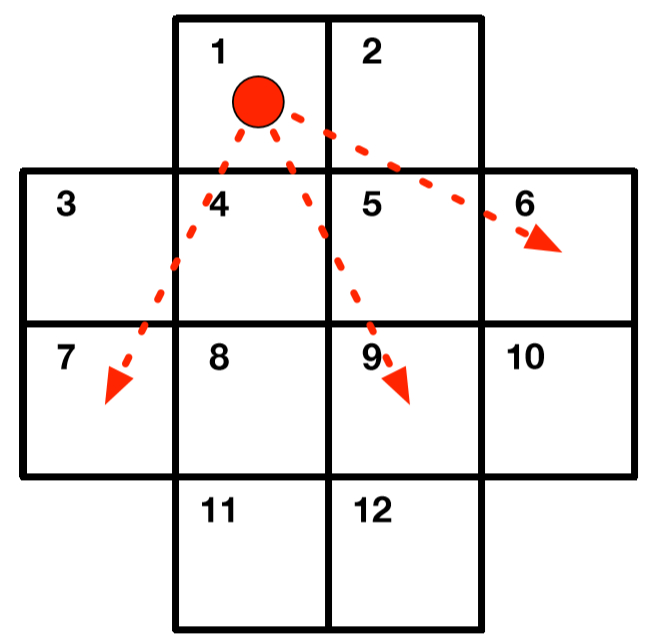
\includegraphics[width=0.35\linewidth]{img/paardensprong.jpg}
	%\captionof{figure}{De mogelijke eerste zetten van het paard}
\end{center}

\begin{enumerate}
	\item Stel dat het paard start op veld 1. Zoek een opeenvolging van bewegingen waarmee het paard elk vierkant juist één keer bezoekt en waarmee het terug eindigt op veld 1.
	
	
	\item Maak een graaf bij dit probleem. We helpen je op weg door het begin van een mogelijke graaf te tekenen. Probeer te interpreteren wat de betekenis is van de knopen en de bogen en vul de graaf verder aan.
	
	%\vspace{2cm}
	\begin{center}
		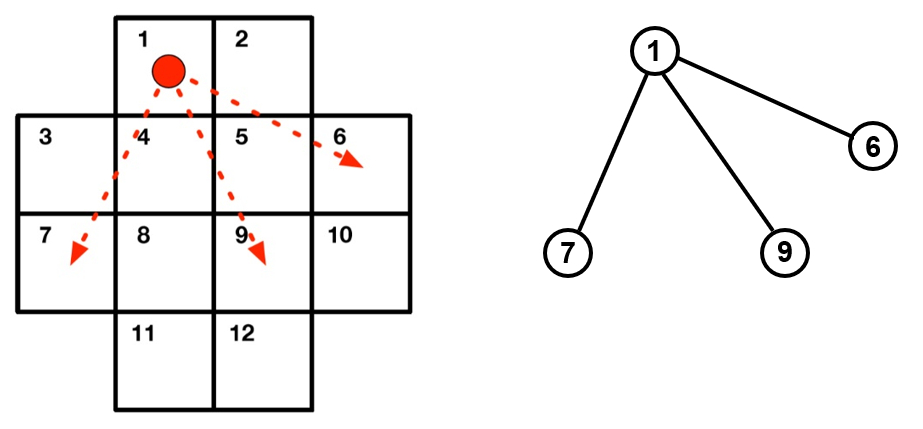
\includegraphics[width=0.8\linewidth]{img/paardenspronggraaf.jpg}
		%\captionof{figure}{De mogelijke eerste zetten van het paard}
	\end{center}
	\vspace{3cm}
	
	\emph{Je kunt dit doen door de vierkanten voor te stellen door knopen. Telkens het paard vanuit een bepaald vierkant op een ander vierkant kan springen, teken je een boog tussen de betreffende knopen. Start met vierkant 1. Vanuit dat vierkant kun je vierkant 6, 7 en 9 bereiken. En zo ga je verder met de andere vierkanten. Je bekomt een figuur zoals hieronder.}
	\begin{center}
		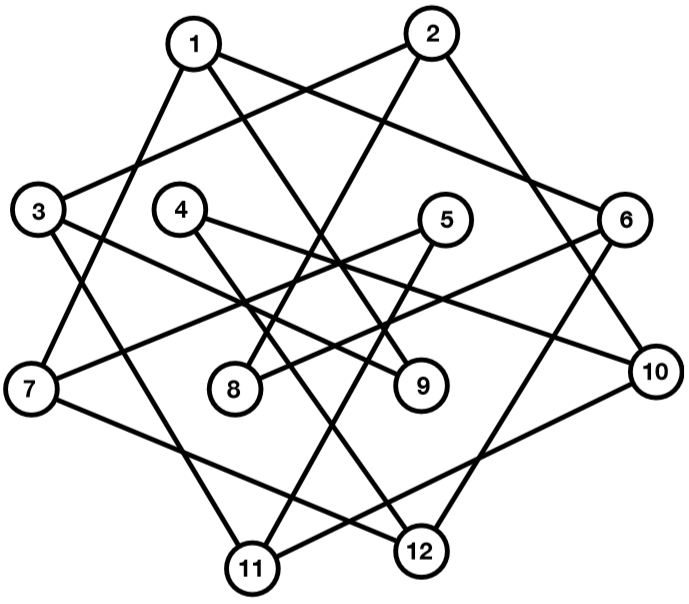
\includegraphics[width=0.5\linewidth]{img/paardenspronggraafvolledig.jpg}
		%\captionof{figure}{De mogelijke eerste zetten van het paard}
	\end{center}

	\item Probeer je graaf nu zo te tekenen dat je zo weinig mogelijk snijdende bogen hebt, maar dat de structuur van de graaf verder gelijk blijft.
	\emph{Je kunt er voor zorgen dat geen enkel paar van bogen snijdend is. Het is dus een planaire graaf.
	\begin{center}
		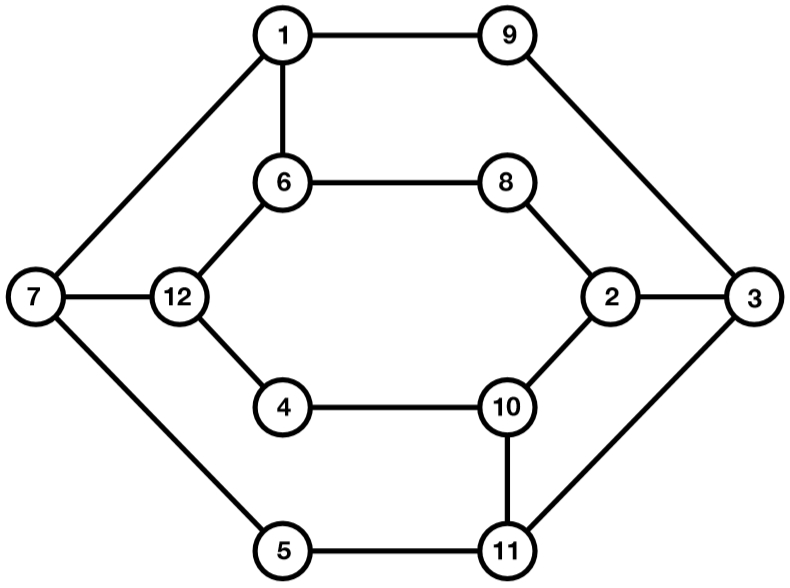
\includegraphics[width=0.5\linewidth]{img/paardenspronggraafvolledigplanair.jpg}
		%\captionof{figure}{De mogelijke eerste zetten van het paard}
	\end{center}
	Wanneer je grafen anders tekent, maar wel de structuur behoudt, dan spreekt men van gelijke grafen.}
	
	\item Lees nu van je graaf de oplossing van de paardenrondgang af. M.a.w. zoek een opeenvolging van bewegingen waarmee het paard elk vierkant juist één keer bezoekt en waarmee het terug eindigt op veld 1.
	
	\emph{Het komt er op aan een hamiltoncykel te vinden in de bovenstaande graaf. Er zijn meerdere oplossingen. Een mogelijkheid is $1-9-3-11-5-7-12-4-10-2-8-6-1$. Dank zij de heldere abstracte voorstelling met grafen kun je heel eenvoudig een oplossing aflezen. Dit voorbeeld toont de kracht van abstractie.}
	
	\begin{figure}[H]
\centering
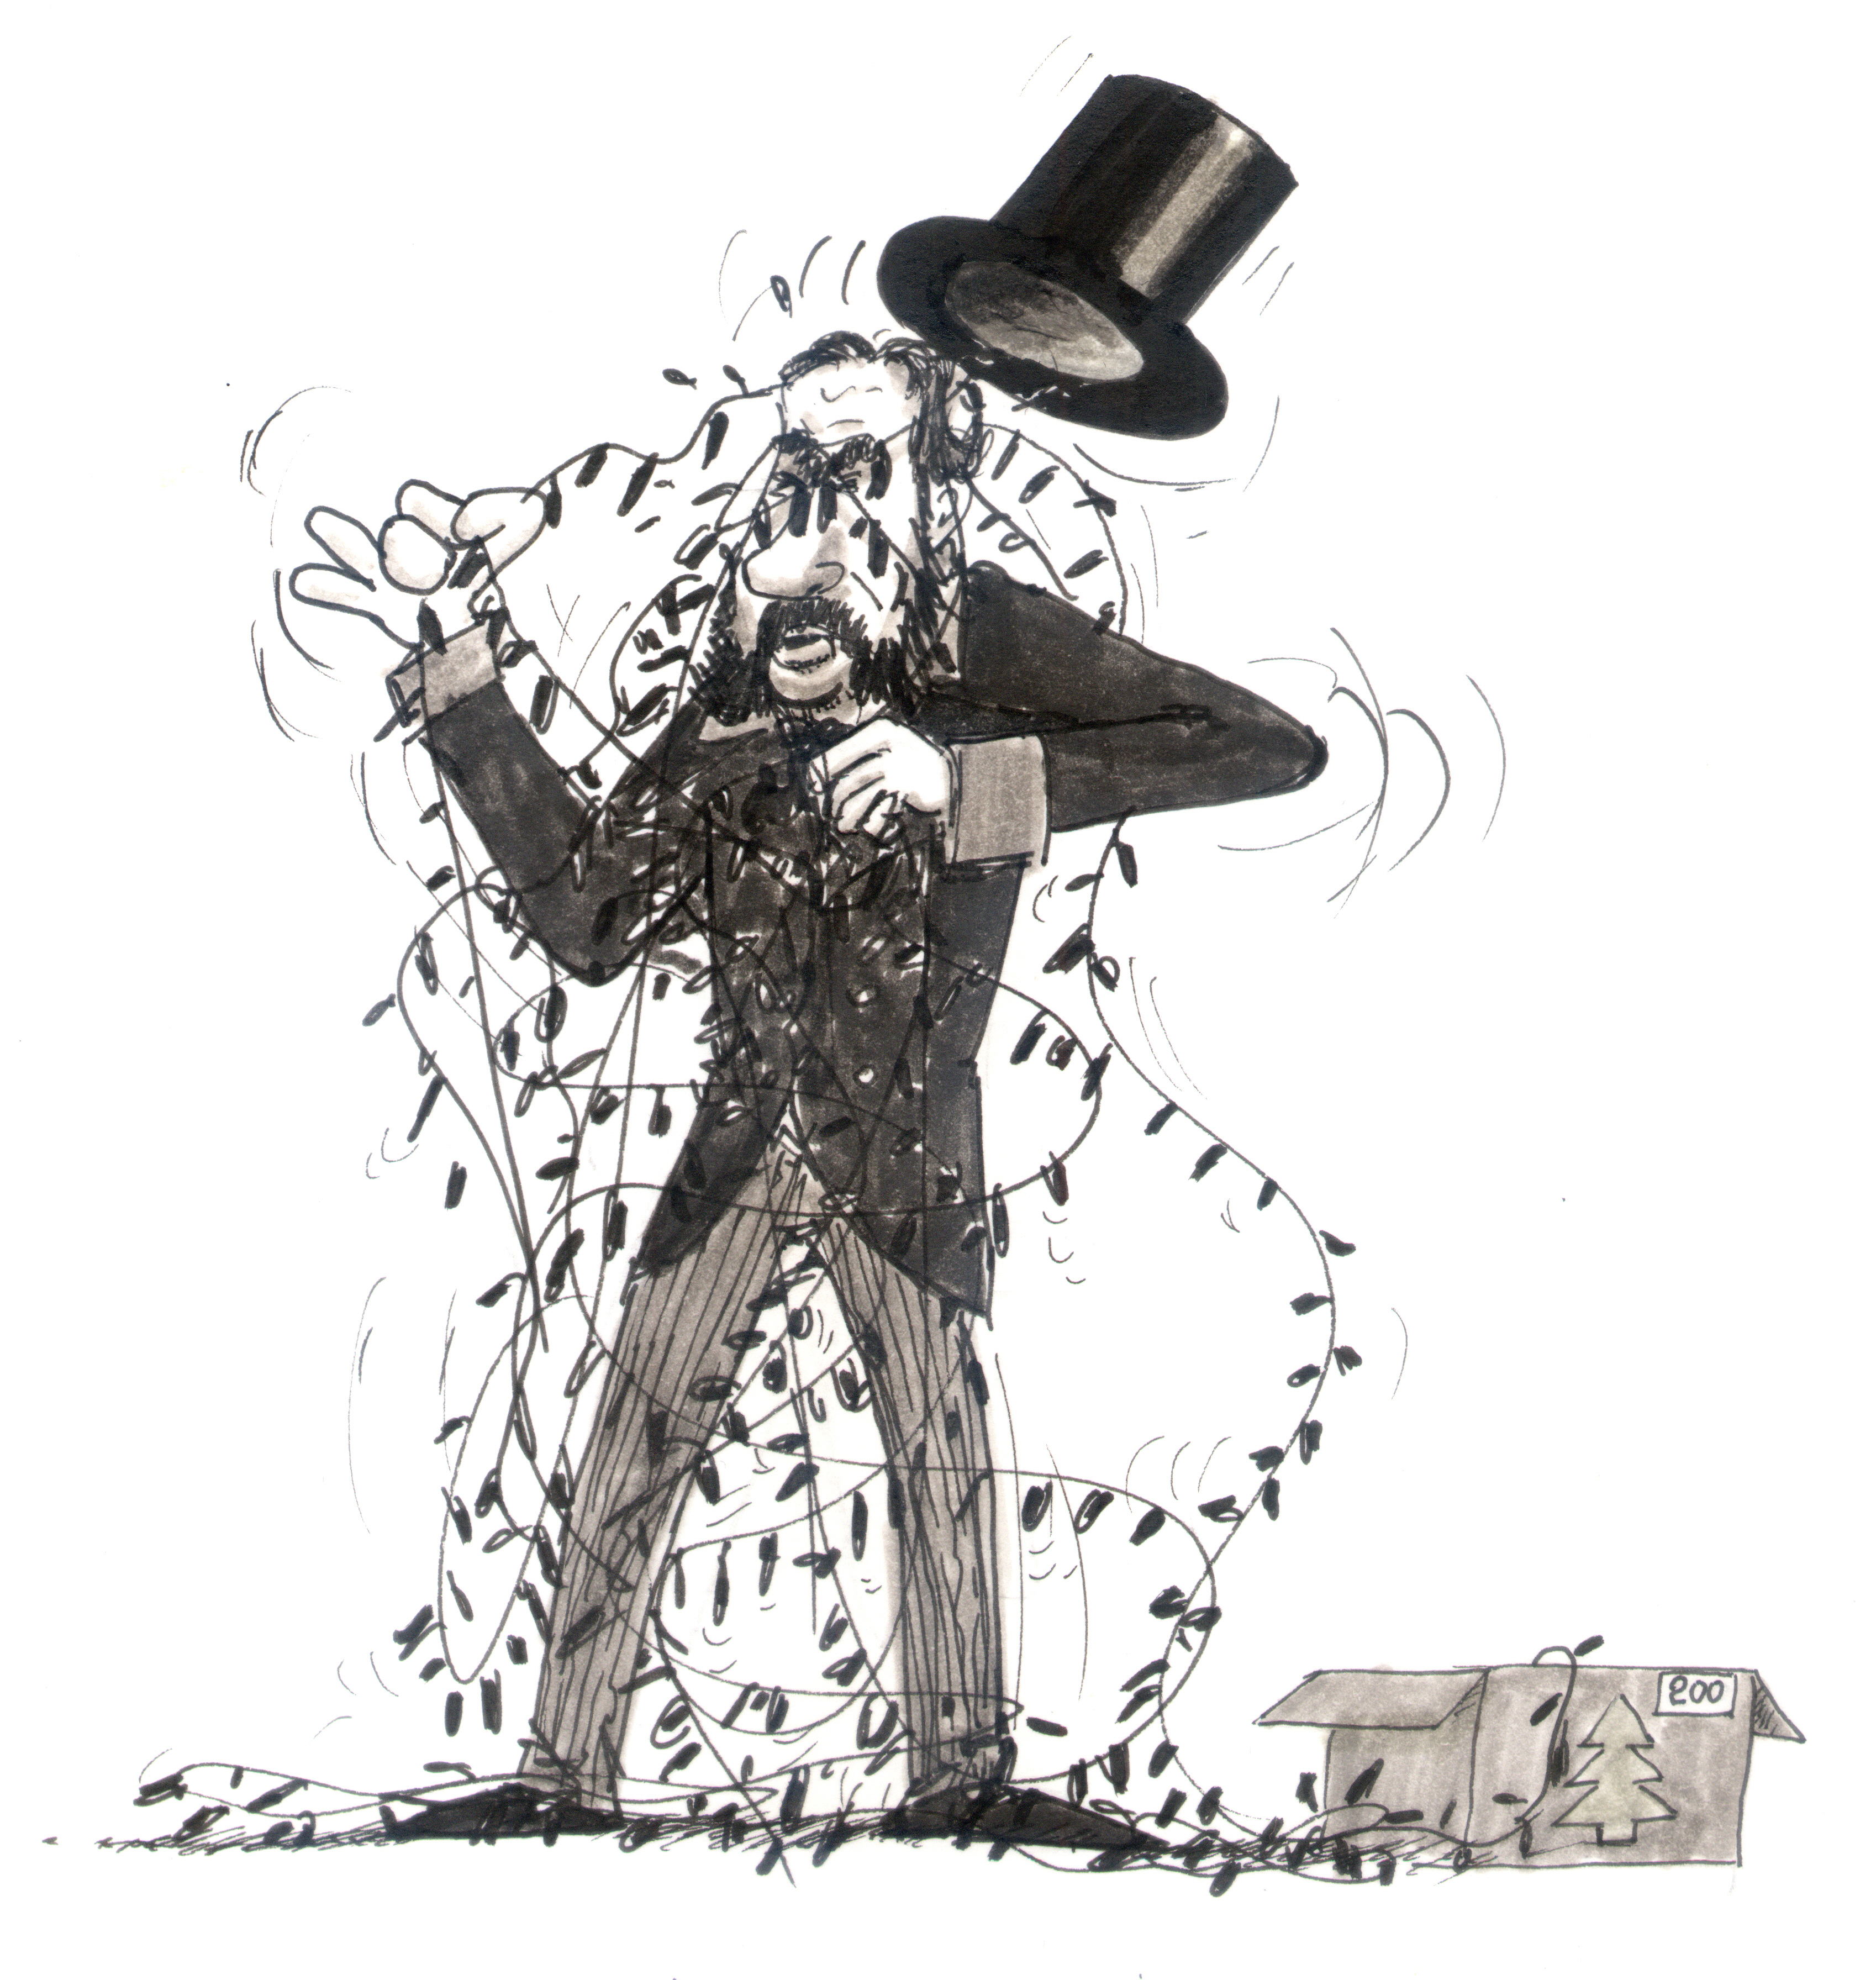
\includegraphics[width=0.8\linewidth]{img/knoop.jpg}
\end{figure} 
	
	\item Kun je een paardenrondgang vinden bij een vierkant $4\times 4$-schaakbord? M.a.w. kun je een opeenvolging vinden van bewegingen waarmee het paard elk vierkant juist één keer bezoekt en waarmee het terug eindigt op veld 1? Verklaar je antwoord.
	\begin{center}
		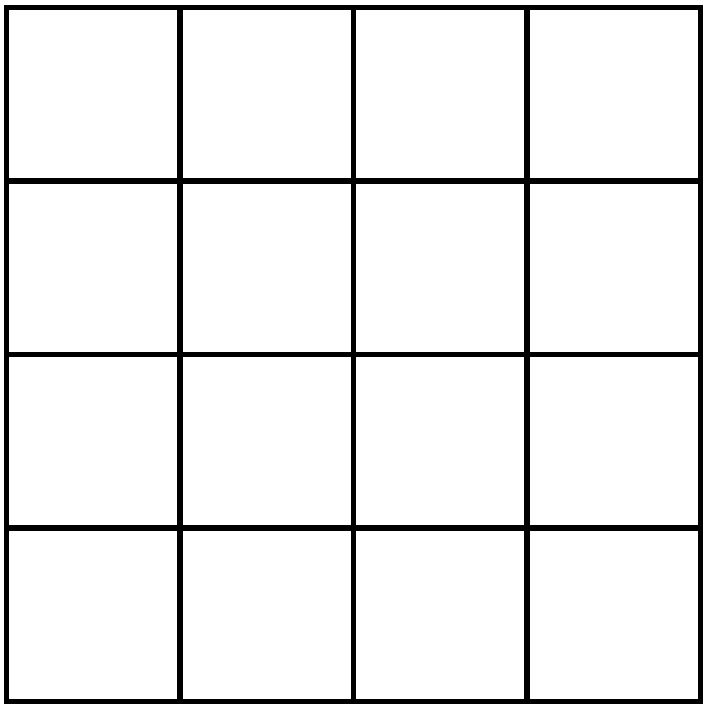
\includegraphics[width=0.3\linewidth]{img/paardenrondgangschaakbord4maal4.jpg}
		%\captionof{figure}{De mogelijke eerste zetten van het paard}
	\end{center}
	
	\emph{Nee, dit lukt niet.
	\begin{center}
		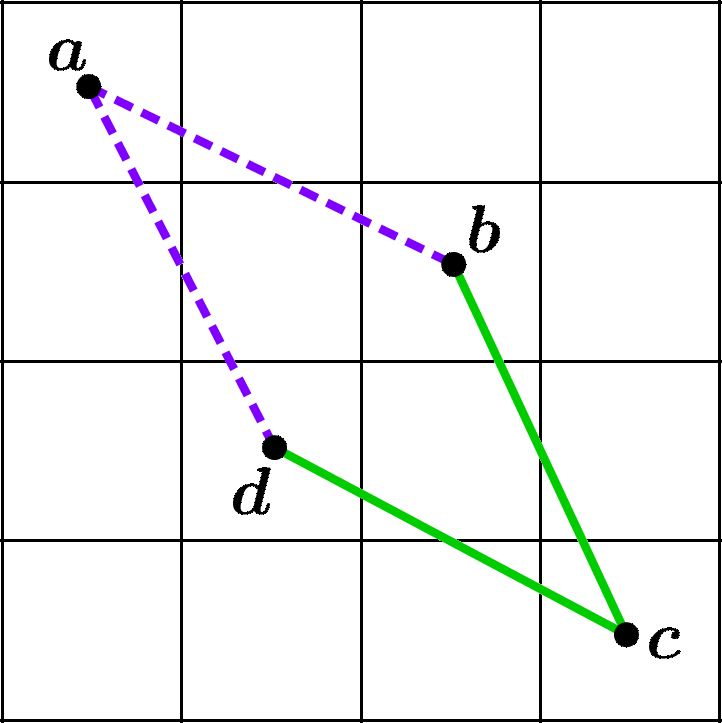
\includegraphics[width=0.27\linewidth]{img/paardenrondgangschaakbord4maal4opl.jpg}
		%\captionof{figure}{De mogelijke eerste zetten van het paard}
	\end{center}
	Sowieso moet je langs $a$ passeren. Je kunt enkel maar in $a$ komen vanuit $b$ of $d$.  Stel dat je vanuit $b$ in $a$ binnenkomt en dat je langs $d$ weer vertrekt uit $a$. Analoog moet je op een bepaald moment langs $c$ passeren, maar je kunt maar in $c$ komen vanuit $b$ of $d$. Je moet dus zowel een beweging maken langs de stippellijnen maken als langs de volle lijnen. Omdat je $d$ en $b$ maar één keer mag passeren, kun je dus niet anders dan in een cykel terecht te komen en daar geraak je niet meer uit.}
	
	%\item Kun je een paardenrondgang vinden op een $2\times 2\times 2$ kubus? Om dit probleem op te lossen: zoek een paardenrondgang op de ontwikkeling van deze kubus.
	
	%\begin{center}
	%	\includegraphics[width=0.4\linewidth]{img/paardenrondgangontwikkelingkubus.jpg}
		%\captionof{figure}{De mogelijke eerste zetten van het paard}
	%\end{center}
	
	
	
	\item Op internet kun je veel paardenrondgangpuzzels vinden. Hieronder zie je een puzzel waarbij het paard op alle witte velden mag bewegen. Vul de witte vakken in met getallen waarmee je de opeenvolging aangeeft van de vakken waar het paard terecht komt. Teken ook een graaf bij deze puzzel (stel elk wit vak voor door een knoop en geef met de bogen aan waar je kunt terechtkomen).
	
	\begin{center}
		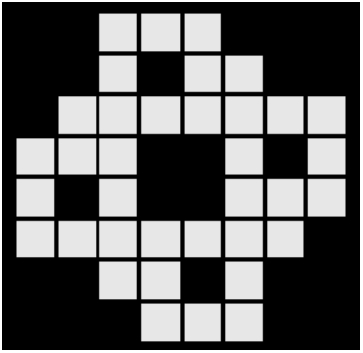
\includegraphics[width=0.4\linewidth]{img/paardenrondgang.jpg}\\
		\footnotesize{Bron: \url{https://www.archimedes-lab.org/knight_tour.html}}
	\end{center}
	
	\emph{Een oplossing: }
	\begin{center}
		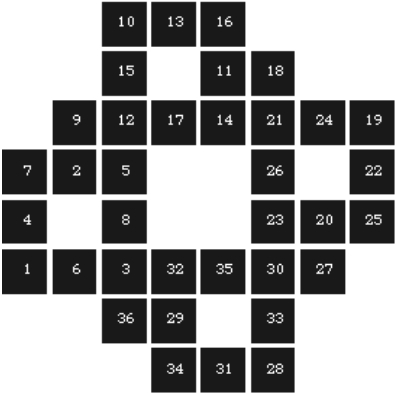
\includegraphics[width=0.35\linewidth]{img/paardenrondgangopl.jpg} 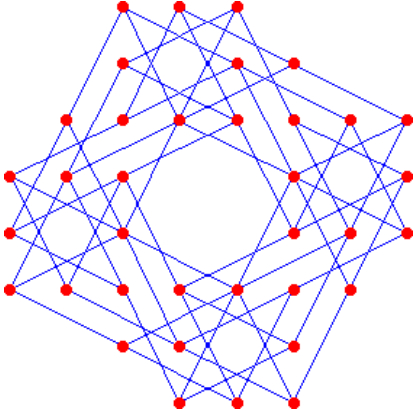
\includegraphics[width=0.35\linewidth]{img/paardenrondganggraaf.jpg}\\
		\footnotesize{\textit{Bron:} \url{https://www.archimedes-lab.org/knight_tour.html}}
	\end{center}



\end{enumerate}



\eindewerktekst

\begin{multicols}{2}
	
De eerste grondige wiskundige studie  van paardenrondgangen werd gedaan in 1759 door Leonhard Euler. Hij bedacht op een klassiek $8\times 8$-schaakbord een open rondgang die eerst de ene helft van het bord afwerkte om daarna de tweede helft op te vullen. 

Bij het standaard $8\times 8$-schaakbord gaat het natuurlijk om veel meer mogelijke bewegingen en velden dan bij de voorbeelden hierboven. Dat betekent dat de grafen die er bij horen veel complexer zijn.  

\begin{center}
	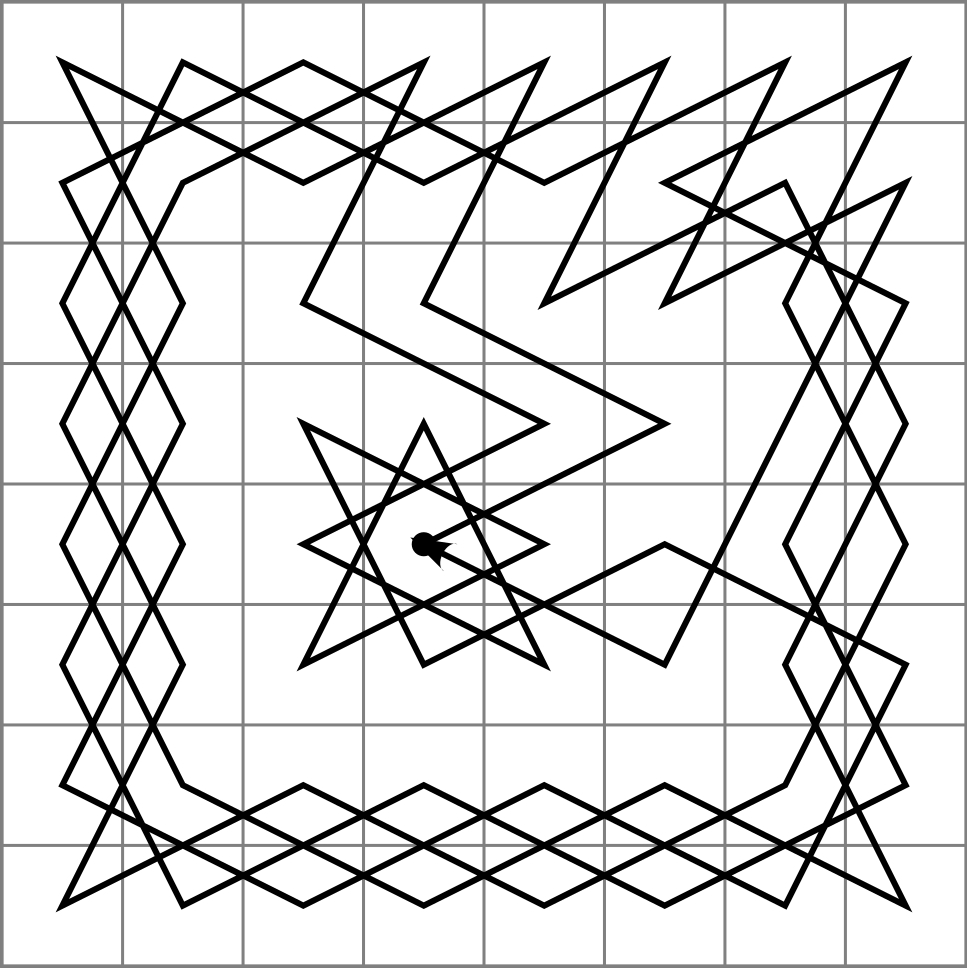
\includegraphics[width=0.9\linewidth]{img/paardenrondgangschaakbord2.jpg}
	\captionof{figure}{Een paardenrondgang op een gewoon schaakbord, opgelost door De Mechanische Turk}
	\label{mechanischeturk}
\end{center}
 
Mogelijke oplossingen worden tegenwoordig meestal gezocht met een computerprogramma. In figuur \ref{mechanischeturk} zie je een paardenrondgang die gevonden werd door de Mechanische Turk, een schaakmachine gebouwd in 1770 door de Hongaarse edelman en uitvinder Wolfgang von Kempelen om indruk te maken op keizerin Maria Theresa van Oostenrijk. Het mechanisme leek in staat om een schaakspel tegen een menselijke tegenstander te spelen en ook een paardenrondgang uit te voeren. In werkelijkheid was het een hoax en zat er een kleine, sterke schaker in.


Leerlingen die iets kennen van programmeren, kun je stimuleren om een programma te schrijven waarmee een paardenrondgang wordt gezocht op een $n\times n$-schaakbord. 


%\subsection{Wanneer is een graaf een hamiltongraaf?}

Op het eerste gezicht zouden we kunnen verwachten dat er een regel bestaat waarmee we kunnen beslissen of een graaf een hamiltongraaf is of niet, maar zo'n eenvoudige regel is er niet. De zoektocht naar nodige en voldoende voorwaarden is een belangrijk onderzoeksdomein binnen grafentheorie. Wat we wel relatief eenvoudig kunnen, is voor bepaalde types van grafen onderzoeken of ze hamiltongrafen zijn. We doen dit in de volgende lesactiviteit voor tweedelingsgrafen.


\end{multicols}

\beginwerktekst{Hamiltongraaf of niet?}

\begin{enumerate}
	\item Is de volgende tweedelingsgraaf een hamiltongraaf?
	\begin{center}
		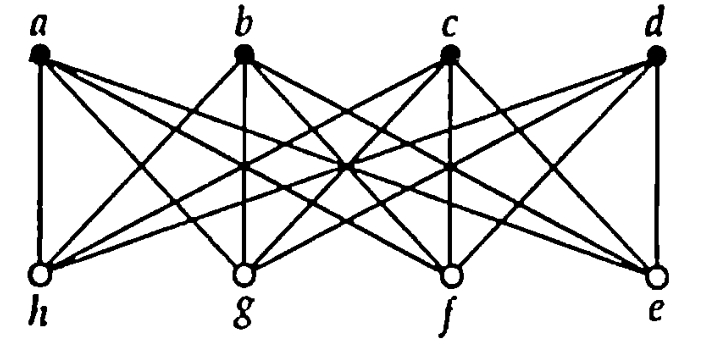
\includegraphics[width=0.5\linewidth]{img/tweedelingsgraaf6.jpg}
	\end{center}
	
	\emph{Ja, $ahbgcfdea$ is een hamiltoncykel.}
	
	\item Toon aan dat een tweedelingsgraaf met een oneven aantal knopen nooit een hamiltongraaf is.
	
	\emph{De knopen van een tweedelingsgraaf kunnen in twee groepen $A$ en $B$ gesplitst worden, zo dat elke boog één uiteinde heeft in $A$ en het andere in $B$. 
	\begin{center}
		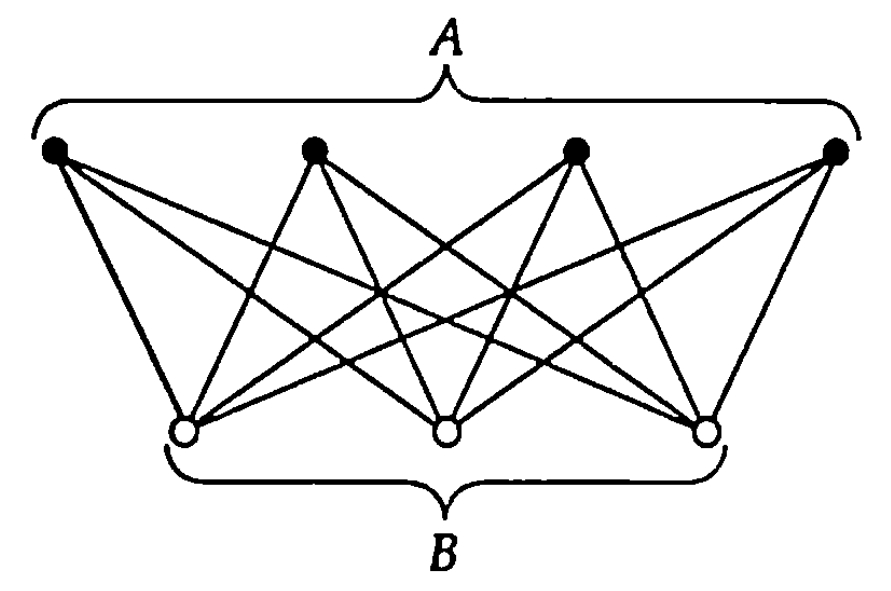
\includegraphics[width=0.5\linewidth]{img/tweedelingsgraaf7.jpg}
	\end{center}
	Elke hamiltoncykel moet alterneren tussen deze twee verzamelingen, waarbij die moet eindigen waar hij begon.  Als een tweedelingsgraaf tegelijk een hamiltongraaf is, moeten $A$ en $B$ hetzelfde aantal knopen hebben. Dit kan niet als het aantal knopen oneven is.}

	\item Is de volgende graaf een hamiltongraaf? Bewijs je antwoord.
	\begin{center}
		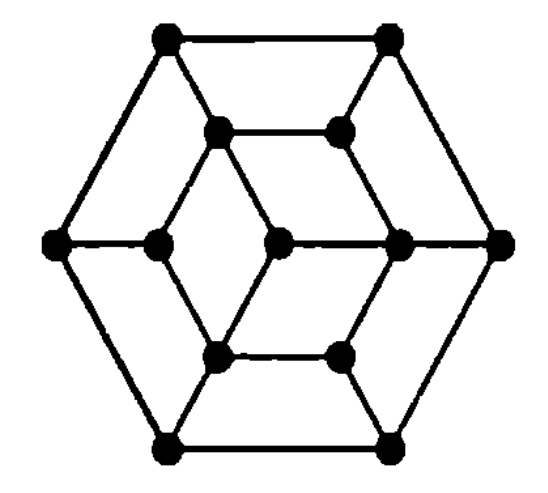
\includegraphics[width=0.3\linewidth]{img/tweedelingsgraaf8.jpg}
	\end{center}
	
	\emph{Als leerlingen er niet in slagen om zelf het antwoord op deze vraag te vinden, kun je hen de tip geven dat ze de vorige vraag kunnen gebruiken. \\Het is geen hamiltongraaf want het is een tweedelingsgraaf met een oneven aantal knopen. Uit de vorige vraag weten we dat deze niet hamiltoniaans kan zijn.}
		\begin{center}
		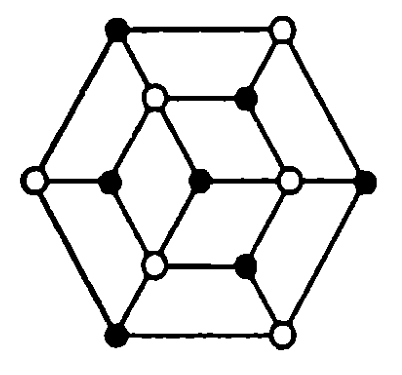
\includegraphics[width=0.3\linewidth]{img/tweedelingsgraaf9.jpg}
	\end{center}
		
	\item Kun je een paardenrondgang vinden op een $5\times 5$-schaakbord?
	
	\emph{Nee, dit lukt niet. Een paardensprong brengt je altijd op een andere kleur van het schaakbord. De graaf die bij dit probleem hoort, is dus een tweedelingsgraaf. Bij een $5\times 5$-schaakbord hebben we een oneven aantal knopen en dus is deze tweedelingsgraaf geen hamiltongraaf.}
	
\end{enumerate}
 

\eindewerktekst
\newpage

\begin{multicols}{2}


\section{Eulergrafen}


In de vorige paragraaf gingen we op zoek naar wandelingen die alle knopen juist één keer aandoen. In deze paragraaf zullen de bogen de rol van de knopen overnemen. We zullen op zoek gaan naar wandelingen die alle bogen van de graaf juist één keer aandoen. We starten met een werktekst over tekenen zonder het potlood op te heffen. Vervolgens gaan we kort in op het historische voorbeeld van Euler over de bruggen van Koningsbergen en voeren we terminologie in. Ten slotte geven we nog andere problemen en toepassingen die neerkomen op het doorlopen van alle bogen van grafen.

\end{multicols}

\beginwerktekst{Zonder je potlood op te heffen}

\begin{nummering}

\item Welke van deze tekeningen kun je maken zonder je potlood op te heffen en zonder meer dan één keer over dezelfde lijn te gaan? En als je moet eindigen in het punt waar je begon?

\begin{center}

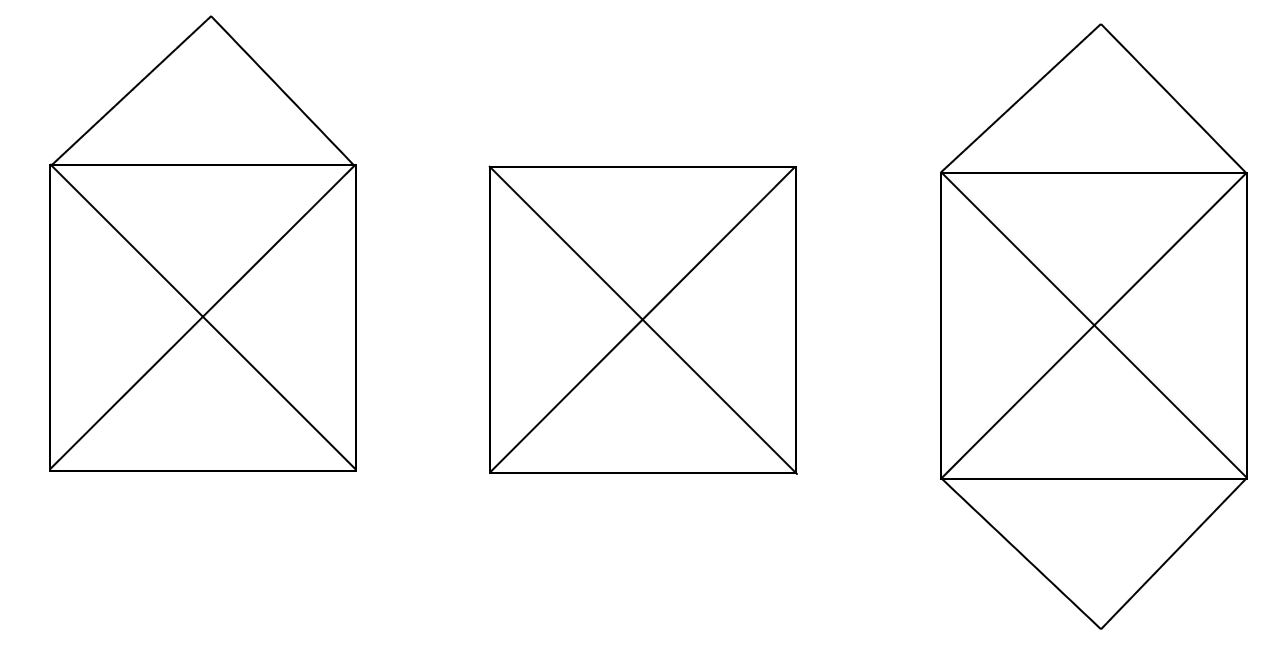
\includegraphics[width=0.65\linewidth]{img/potlood1.jpg}

\end{center}
\emph{De eerste is mogelijk. Je moet in één van de onderste punten beginnen en in het andere onderste punt eindigen. Maar als je in hetzelfde punt moet beginnen en eindigen lukt het niet.}


\emph{De tweede lukt niet.}

\emph{Bij de derde is het mogelijk. Je begint en eindigt hier in hetzelfde punt. Je kunt zelfs kiezen in welk punt je start.}

\emph{Hieronder laten we voorbeelden zien van tekeningen zonder het potlood op te heffen, voor de twee gevallen waarbij het gaat. We sluiten de tekening niet; we laten een beetje spatie zodat je kunt zien waar we begonnen en eindigden. Het onderscheid tussen begin- en eindpunt is niet belangrijk.}

\begin{center}
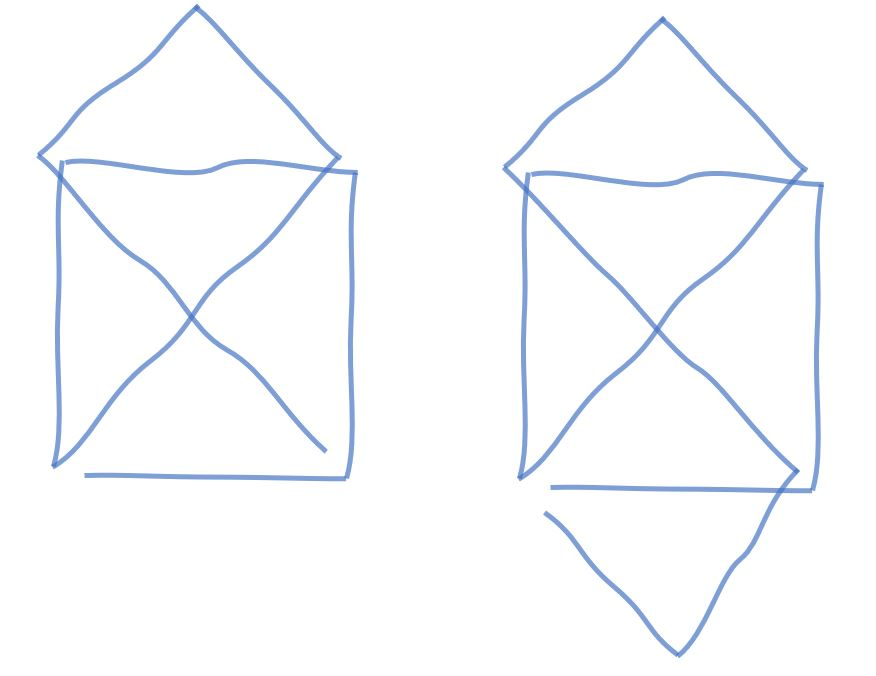
\includegraphics[width=0.35\linewidth]{img/potlood3.jpg}
\end{center}

\item Formuleer de vorige opgave als een opgave over grafen. In de grafentheorie spreekt men over `wandelen' in plaats van over tekenen zonder het potlood op te heffen.

\emph{We voegen knopen toe zodat de lijnen bogen worden van een graaf. We zouden ook nog in het midden een knoop kunnen plaatsen. Voor het al of niet oplosbaar zijn, maakt dit geen verschil (zie verderop). We bekijken de diagonalen van het vierkant als bogen die toevallig getekend zijn als snijdende lijnstukken.}

\begin{center}
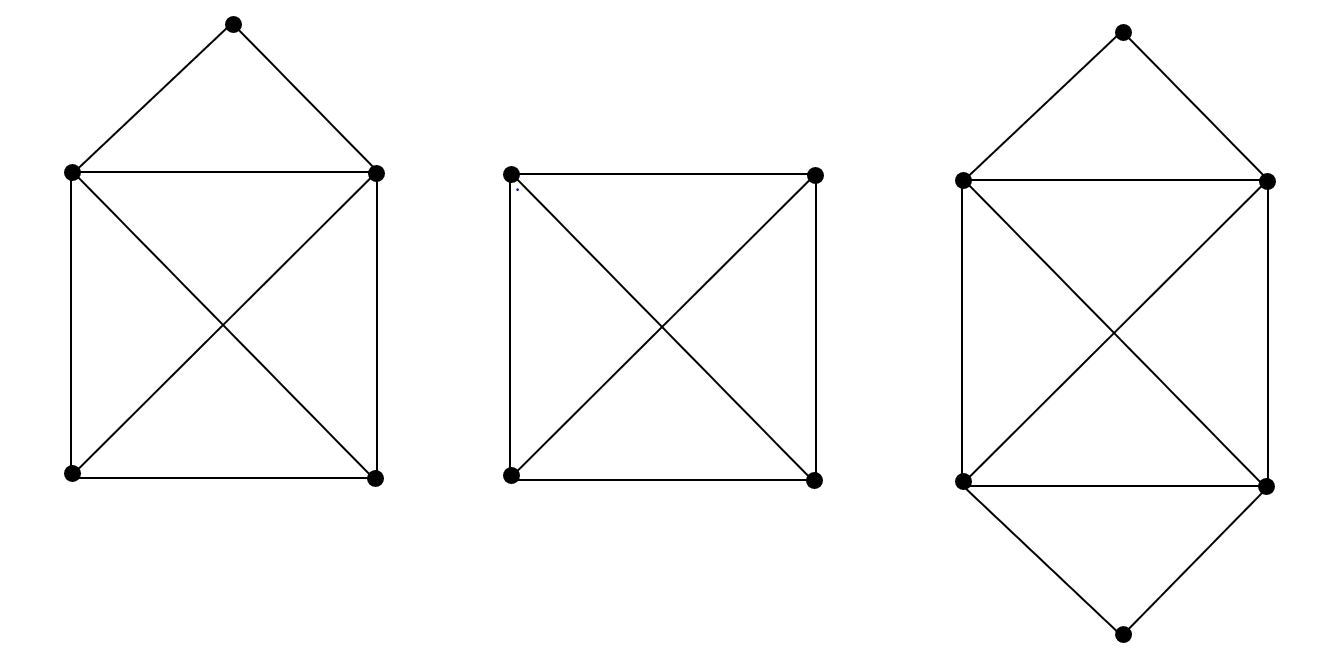
\includegraphics[width=0.65\linewidth]{img/potlood2.jpg}
\end{center}

\emph{De opgave luidt dan: kun je een wandeling maken zodat je alle bogen van de graaf juist één keer aandoet en wel of niet eindigt in de knoop waar je vertrok?}

\item Zoek een verband tussen het bestaan van een dergelijke wandeling en de graden van de knopen van deze grafen.

\emph{We noteren bij elke knoop zijn graad. Bij de eerste tekening zijn er twee knopen met oneven graad en daar moesten we de wandeling (de potloodlijn) beginnen en eindigen. Een knoop waar we enkel (een keer of meerdere keren) voorbij wandelen, kan enkel een even graad hebben want telkens komen we toe op een boog en gaan we verder op een andere boog. Dit verklaart waarom de tweede tekening niet mogelijk is. Bij de derde zijn alle graden van de knopen even. Hier vertrek je en eindig je in dezelfde knoop. Ook in die knoop moet het aantal bogen inderdaad even zijn: je hebt er de boog waarop je begint, telkens twee bogen als je er voorbijkomt en nog één boog waarop je eindigt.}

\begin{center}
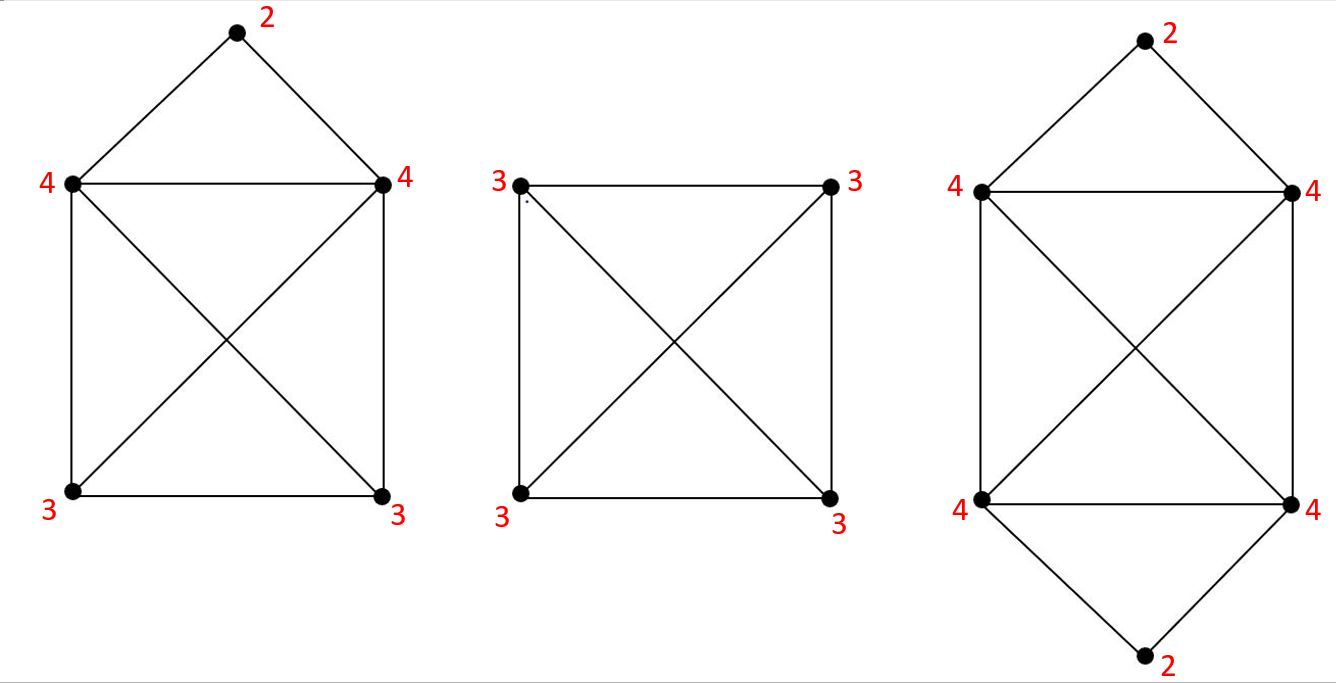
\includegraphics[width=0.65\linewidth]{img/potlood5.jpg}
\end{center}

\end{nummering}

\eindewerktekst

\begin{multicols}{2}

We voeren enkele benamingen in.

Een wandeling langs opeenvolgende bogen, zonder dat dezelfde boog herhaald wordt, noemen we een \emph{spoor} (Engels: \emph{trail}). Een \emph{circuit} is een wandeling langs opeenvolgende bogen, zonder dat dezelfde boog herhaald wordt en waarbij men eindigt in de startknoop. Men zegt ook dat een circuit een `gesloten' spoor is. Spoor en circuit zijn de tegenhangers van pad en cykel van de vorige paragraaf, waarbij nu de bogen de rol spelen die de knopen toen speelden... 

Een \emph{eulercircuit} is een circuit dat over alle bogen van de graaf gaat. Een graaf waarin een eulercircuit bestaat heet een \emph{eulergraaf}. 

Een \emph{eulerspoor} is een `open' spoor dat over alle bogen van de graaf gaat. Een graaf waarin een eulerspoor bestaat, heet een \emph{traverseerbare graaf} (soms lees je ook: een semi-eulergraaf).

In de vorige werktekst was de eerste graaf traverseerbaar, de derde was een eulergraaf en de tweede was noch een eulergraaf noch een traverseerbare graaf.

Laat de leerlingen voorbeelden geven van grafen met tien knopen: een eulergraaf, een traverseerbare graaf en een graaf die dit niet is.

De naam eulergraaf komt van de Zwitserse wiskundige Leonhard Euler (18de eeuw). Euler was zeer creatief en ongelooflijk productief. Als we de Nederlandstalige Wikipedia mogen geloven: ``Euler heeft zoveel geschreven, dat het met de hand overschrijven van al zijn werken naar schatting vijftig jaar zou duren bij acht uur schrijven per dag.'' Zijn probleem van de `bruggen van Koningsbergen' wordt beschouwd als het ontstaan van de grafentheorie.

De stad Koningsbergen (of in het Duits Königsberg) was de hoofdstad van Pruisen. Na de tweede wereldoorlog werd de stad toegevoegd aan de Sovjet-Unie en herdoopt tot Kaliningrad. Nu is Kaliningrad een stukje Rusland, gekneld tussen Polen en Litouwen.

Er waren ten tijde van Euler zeven bruggen over de rivier Pregel, die de verschillende stadsdelen met elkaar verbonden (figuur \ref{euler1}).

\begin{center}
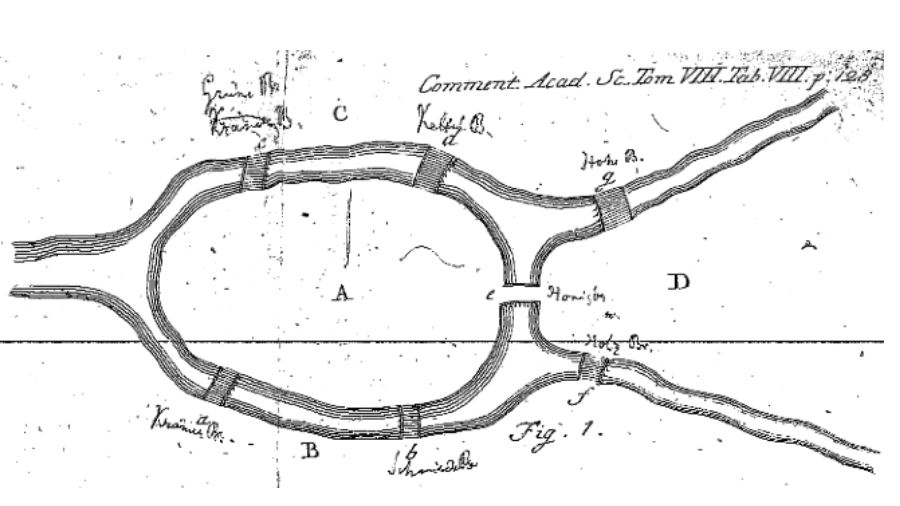
\includegraphics[width=\linewidth]{img/Eulerbruggen.jpg}
\captionof{figure}{Tekening door Euler van de zeven bruggen}
\label{euler1}
\end{center}

Het probleem dat Euler oploste, luidde: "Ontwerp een wandeling in Koningsbergen die juist één keer over elke brug gaat".

Euler maakte hier een graaf van (misschien wel de eerste graaf uit de geschiedenis). Hij stelde elk stadsdeel voor als een knoop en elke brug als een boog (figuur \ref{euler2}).

\begin{center}
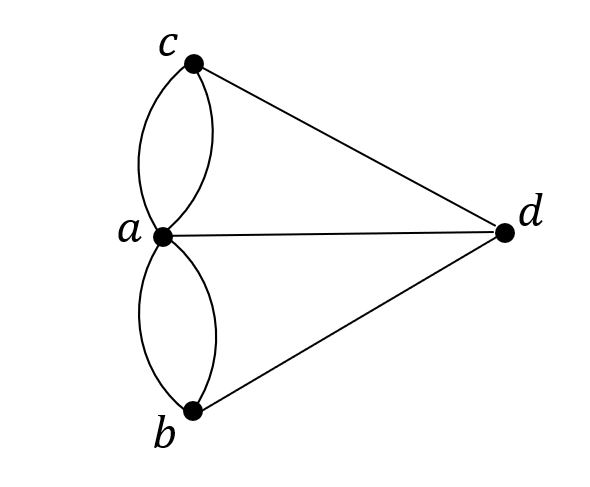
\includegraphics[width=0.6\linewidth]{img/Eulerbruggen2.JPG}
\captionof{figure}{De bruggen als bogen van een graaf}
\label{euler2}
\end{center}

Meteen valt op dat dit geen graaf is zoals we tot nu toe tegenkwamen. Nu heb je tussen sommige knopen meer dan één boog. We spreken van een \emph{multigraaf}. De graad van een knoop van een multigraaf, het aantal bogen dat in die knoop toekomt, kan groter zijn dan het aantal buren. Ook in een multigraaf kun je, helemaal analoog, (euler)sporen en (euler)circuits definiëren. Een eulermultigraaf is dan een multigraaf waarin een eulercircuit bestaat en een traverseerbare multigraaf een multigraaf waarin een eulerspoor bestaat.

Het probleem dat Euler moest oplossen, kan vertaald worden als: is de multigraaf van de situatie in Koningsbergen traverseerbaar?

Na de vorige werktekst kunnen de leerlingen dit vlot oplossen. Het komt op hetzelfde neer als de vraag om alle bogen van deze graaf te tekenen zonder het potlood op te heffen. De graden van de knopen zijn: $\deg(a)=5, \deg(b)=3, \deg(c)=3, \deg(d)=3$. Het lukt niet want in een traverseerbare (multi)graaf mogen er maar twee knopen zijn met een oneven graad: de start- en de eindknoop van de wandeling (van het spoor).

Euler formuleerde twee stellingen, die wij nu als volgt formuleren. Hijzelf sprak natuurlijk niet van `euler'spoor en `euler'graaf.

\begin{stellingkadertwee}{Stelling}{}{Een samenhangende (multi)graaf is traverseerbaar als en slechts als er juist twee knopen zijn met oneven graad. Deze knopen zijn dan het begin- en eindpunt van het eulerspoor.}

\end{stellingkadertwee}

\begin{stellingkadertwee}{Stelling}{}{Een samenhangende (multi)graaf is een euler(multi)graaf als en slechts als alle knopen een even graad hebben.}
\end{stellingkadertwee}

Hijzelf bewees de implicatie $\Rightarrow$, met andere woorden het feit dat de voorwaarde in verband met de graden van de knopen nodig is. De redenering is dezelfde als bij de tekeningen zonder het potlood op te heffen in de vorige activiteit. Het feit dat het over een multigraaf gaat in plaats van een graaf, verandert hier niets aan. Behalve in de begin- en eindknoop, heb je in elke knoop, voor elke keer dat je er voorbij wandelt, een boog waarop je toekomt en een boog waarop je verdergaat. Daardoor is de graad even. 

De andere implicatie is pas in de 19de eeuw bewezen door Carl Hierholzer. We verwijzen voor dit mooie, constructieve bewijs naar Perucca (2019).

In de volgende werkteksten ontmoet je enkele andere situaties die ook te modelleren zijn door al dan niet traverseerbare multigrafen.

\end{multicols}

\beginwerktekst{De moord}

(Naar: Benjamin e.a., 2015.)

\begin{center}
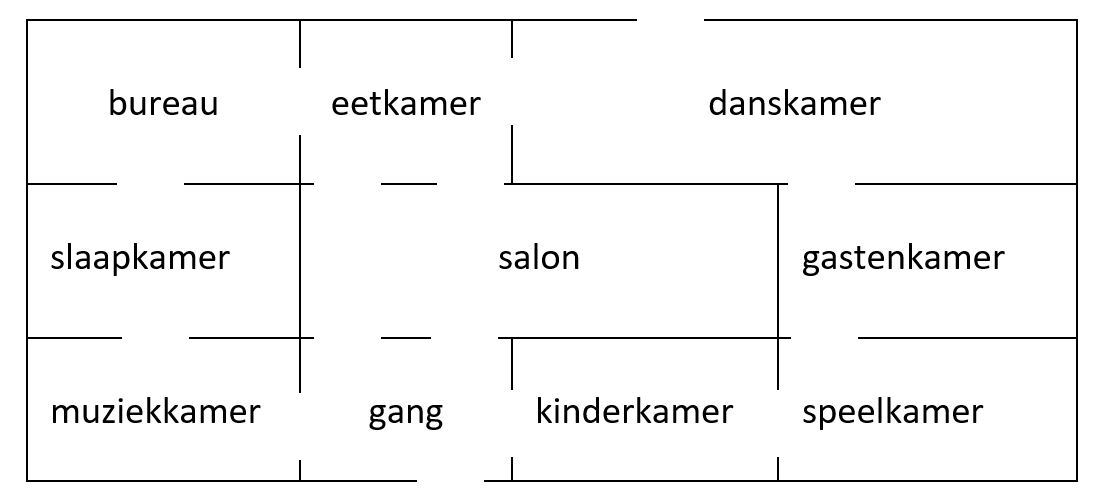
\includegraphics[width=0.6\linewidth]{img/moord1.jpg}
\end{center}

Inspecteur Pratt moet de moord op Dr. Black oplossen. Het lijk van Dr. Black is in het bureau teruggevonden. De buttler beweert dat hij iemand gezien heeft die in het bureau binnenging en via dezelfde deur het bureau weer verliet. De inspecteur ondervraagt Mrs. Peacock en die zegt: ``Ik ben niet degene die Dr. Black gezien heeft, want ik ben door de voordeur (aan de gang) binnengekomen en via de achterdeur (aan de danskamer) weer buiten gegaan en ik ben juist één keer door elke deur gegaan.'' Is iemand aan het liegen?

\emph{Maak een multigraaf waarbij de kamers (en ook de buitenwereld) de knopen zijn, en de deuren de bogen. Mrs. Peacock beweert dat ze een eulercircuit heeft afgelegd, van de buitenwereld naar de buitenwereld. Dit zou enkel mogelijk zijn als de graden van alle knopen even zijn. Maar: de gang en de danskamer worden voorgesteld door knopen met oneven graden... De graaf is wel traverseerbaar maar dan moet je vertrekken en eindigen in de gang en de danskamer, de enige knopen met oneven graad. Mrs. Peacock liegt. Dit maakt haar natuurlijk verdacht, al is dit nog geen hard bewijs dat zij de moord pleegde.}

\eindewerktekst

\beginwerktekst{De postbode}

\begin{nummering}
\item Patrick de postbode wil in de wijk hieronder de post ronddelen. Hij wil een route uitstippelen die juist twee keer langs elke straat passeert, zodat hij niet telkens de straat moet oversteken. Het liefst eindigt hij waar hij begonnen is. Is dit mogelijk? Modelleer met een graaf en help Patrick.

\begin{center}
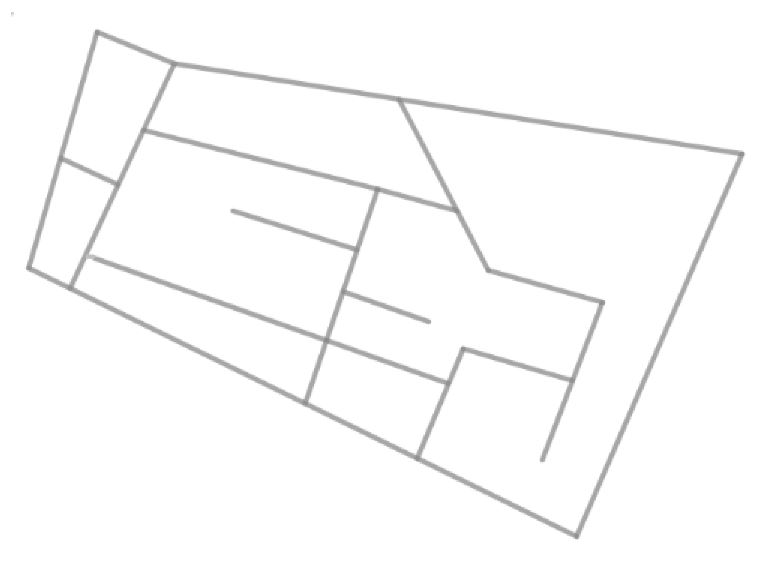
\includegraphics[width=0.4\linewidth]{img/stratenplan.JPG}
\end{center}

\emph{Je maakt een multigraaf waarbij elke straat voorgesteld wordt door twee bogen. De knopen zijn de kruispunten van twee of meer straten en de eindpunten van de doodlopende straten. Waar een straat een knik maakt, is het niet nuttig om een knoop te plaatsen.}

\begin{center}
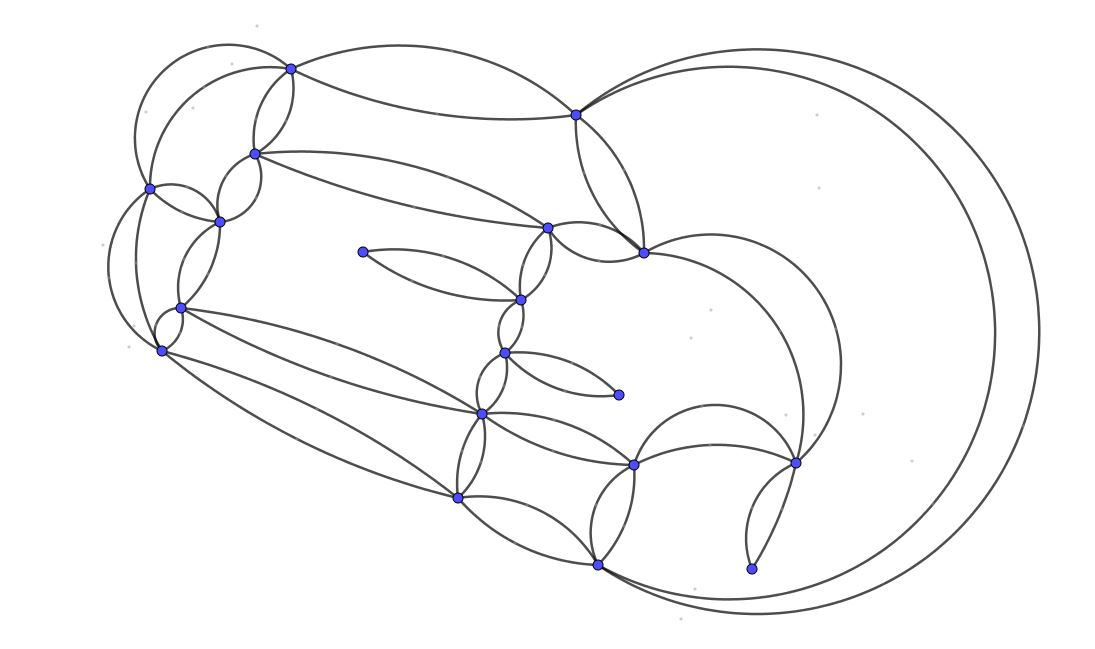
\includegraphics[width=0.5\linewidth]{img/multigraafstratenplan.JPG}

\end{center}

\emph{Een dergelijke multigraaf is een eulermultigraaf want de graad van elke knoop is even. Dus: het gaat! We laten het uitstippelen van een concrete route over aan de lezer.}

\item Maakt het concrete stratenpatroon iets uit?

\emph{Voor het bestaan van een dergelijke route maakt het eigenlijk niet uit. Omdat je een multigraaf maakt waarbij elke straat omgezet is in twee bogen tussen dezelfde knopen, zullen alle graden even zijn, hoe de straten ook lopen. Voor het concreet uitstippelen van de route kan de complexiteit van het stratenplan de opdracht natuurlijk wel bemoeilijken.}
%Het algoritme van Fleury zegt dat je de route kunt vinden door de bogen op de route te kleuren en steeds, zolang het kan, bogen te vermijden die 'bruggen' zijn in de deelboom van de nog niet gekleurde bogen. Ik wil dit hier echter niet uitleggen...
\end{nummering}

\eindewerktekst

\beginwerktekst{Zo weinig mogelijk je potlood opheffen}

\begin{nummering}

\item{Hoeveel keer moet je minstens je potlood optillen om de volgende figuren te tekenen?}

\begin{center}
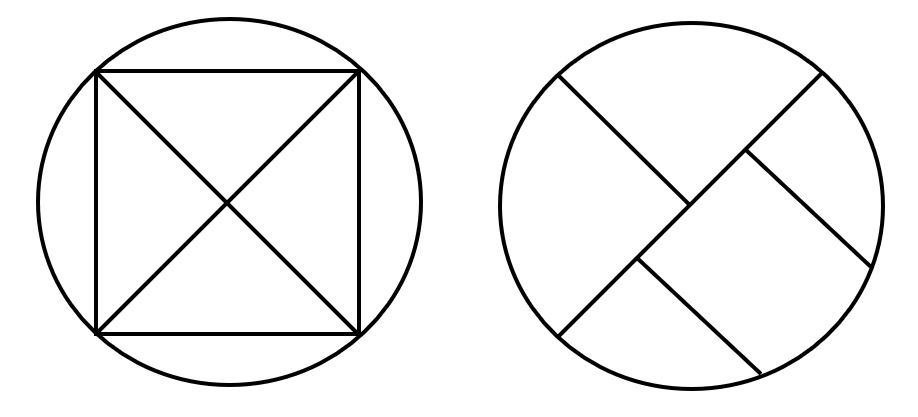
\includegraphics[width=0.55\linewidth]{img/potloodheffen1.JPG}
\end{center}

\emph{De eerste figuur lukt door één keer tussendoor het potlood op te heffen. Voor de tweede tekening is het nodig om drie keer tussendoor het potlood op te heffen.}

\item Als je deze tekeningen opvat als grafen: hoeveel knopen met oneven graad hebben ze? Waarom kunnen ze niet getekend worden zonder het potlood op het heffen?

\emph{De eerste heeft vier knopen van oneven graad, de tweede acht. Enkel bij nul of twee knopen met oneven graad kun je de graaf tekenen zonder het potlood op te heffen.}

\item Bewijs: een graaf met $k$ knopen met oneven graad, kun je tekenen door $\frac{k}{2} - 1$ keer het potlood op te heffen. Tip: voeg bogen toe om er een traverseerbare multigraaf van te maken.

\emph{Merk op dat $\frac{k}{2} - 1$ steeds een natuurlijk getal is, want het aantal knopen van oneven graad is steeds even. Voeg in een kleur $\frac{k}{2} - 1$ bogen toe waarbij je knopen van oneven graad twee aan twee verbindt. Hiermee worden $2\cdot \left(\frac{k}{2} - 1\right)=k-2$ oneven graden omgezet in even graden. Er blijven nog twee knopen van oneven graad over. De graaf is traverseerbaar geworden en kun je dus met een Eulerpad in één potloodstreep tekenen. Vervang hierin de gekleurde bogen door het opheffen van het potlood (teken de gekleurde bogen in de lucht).}

\end{nummering}


\eindewerktekst


\begin{multicols}{2}




%\begin{opsomming}
%\item multigrafen (meer dan één boog mogelijk tussen twee toppen, wat niet kan in een gewone ('enkelvoudige') graaf),
%\item wandelingen,
%\item sporen (geen herhalende bogen),
%\item circuits (gesloten spoor),
%\item eulerspoor/-circuit (spoor/circuit dat elke boog bevat),
%\item eulergraaf (graaf die een eulercircuit bevat),
%\item traverseerbare (Nederlands woord??) graaf (graaf die een eulerspoor bevat),
%\item pijlen (gerichte bogen)
%\item $\ldots$
%\end{opsomming}
%Een belangrijk typevoorbeeld is dat van de bruggen van Koningsbergen. Bedoeling is ook hier dat telkens met kleine (evt. zelfs contextloze) oefeningetjes de begrippen worden geïntroduceerd.

%Het is redelijk eenvoudig om na te gaan of een graaf een eulergraaf is: de graad van elke top moet even zijn (bewezen door Hierholzer, zie ontmoeting Lage Landen). We verwijzen voor dit bewijs naar Petrucca (vorig nummer). \\Een graaf is traverseerbaar(??) als hij juist twee toppen met oneven graad heeft.

%We maken enkele kleine oefeningen m.b.t. deze begrippen en laten verschillende soorten toepassingen zien o.a. controleronde door een huis, misdaad, ophalen huisvuil.

%\section{Topologisch sorteren}
%In gerichte grafen wordt een lineaire ordening van de knopen aangebracht. Komt bijvoorbeeld voor bij het plannen van taken waarbij door beperkingen de ene taak vóór de andere moet worden uitgevoerd. Weer behandelen we kleine probleempjes, zoals bijvoorbeeld een werkrooster opstellen, woorden sorteren in een woordenboek.




%\section{Breedte-eerst-problemen}
%Dit gaat over grafen die steeds verder uitwaaien, zoals een boom met een wortel en dan steeds meer vertakkingen.\\ Breadth-first search (BFS) is een zoekalgoritme op een graaf dat begint bij de wortel (begintop) van de graaf en dat voor elk van de kinderen kijkt of het de oplossing is en dan voor elk van die kinderen dit proces uitvoert totdat de gewenste oplossing gevonden is. \\
%Een typische toepassing is een schuifpuzzel of letters in een woord veranderen om naar een ander woord over te gaan.

\section{Minimale opspannende boom}

Een belangrijk aspect van grafentheorie is het werken met algoritmen. Een algoritme is een heel precies recept om stap voor stap naar een oplossing te gaan. Een recept voor mayonaise kun je bekijken als een algoritme: als je met de juiste ingrediënten het recept correct uitvoert, dan heb je op het einde mayonaise. Veel stappenplannen uit de algebra zijn ook algoritmen: de methode van Gauss en Jordan om een stelsel van eerstegraadsvergelijkingen op te lossen, het berekenen van de oplossingen van een tweedegraadsvergelijking met de discriminant, de staartdeling, enzovoort. Een algoritme kun je vertalen in een programmeertaal en door een computer laten uitvoeren. Dit is nodig bij grafentheorie, omdat de grafen waar men in de praktijk mee te maken krijgt $-$ in tegenstelling tot de kleine graafjes die wij hier gebruiken om de begrippen uit te leggen $-$ reusachtig groot zijn. Een routeplanner zoekt voor de gebruiker de kortste route in het wegennetwerk, dat je kunt modelleren door een heel grote graaf.

Om de idee van een algoritme in de grafentheorie aan te brengen, zullen we op zoek gaan naar de kortste of goedkoopste verbinding van alle knopen van een gegeven graaf met elkaar. Denk bv. aan een computernetwerk: de knopen zijn computers en die moeten allemaal met glasvezels met elkaar verbonden worden, niet noodzakelijk rechtstreeks.

Om dit preciezer te definiëren, voeren we een aantal definities in. Je kunt die begrippen aan de leerlingen uitleggen. Je zou ook de definities aan de leerlingen kunnen geven en hen zelf vragen om voorbeelden en tegenvoorbeelden te bedenken (zie paragraaf 3).

Een graaf $H$ is een \emph{deelgraaf} van een graaf $G$ als alle knopen van $H$ ook knopen zijn van $G$ en alle bogen van $H$ ook bogen zijn van $G$.

Een deelgraaf $H$ van $G$ die alle knopen van $G$ bevat, is een \emph{opspannende} deelgraaf van $G$.

\begin{center}
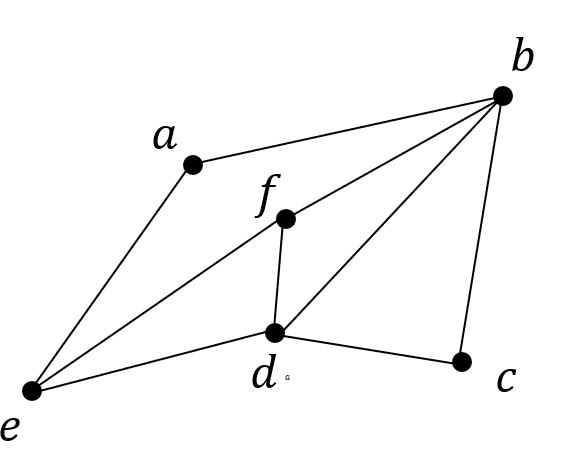
\includegraphics[width=0.6\linewidth]{img/deelgraaf1.jpg}
\captionof{figure}{Een graaf $G$}
\label{boom1}
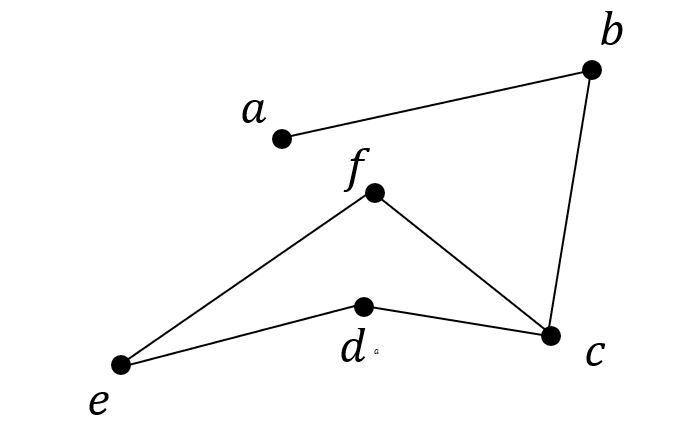
\includegraphics[width=0.7\linewidth]{img/deelgraaf6.jpg}
\captionof{figure}{Geen deelgraaf van $G$}
\label{boom2}
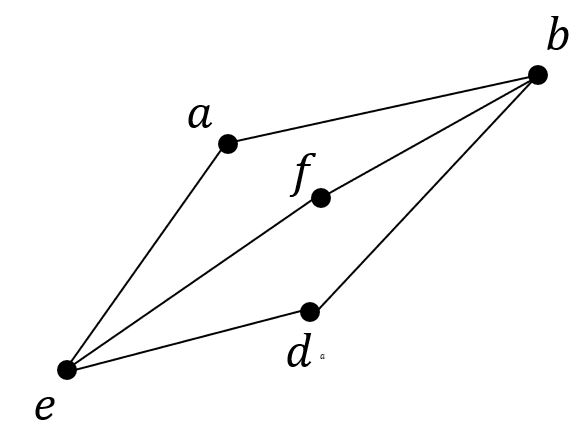
\includegraphics[width=0.6\linewidth]{img/deelgraaf7.jpg}
\captionof{figure}{Een deelgraaf van $G$}
\label{boom3}
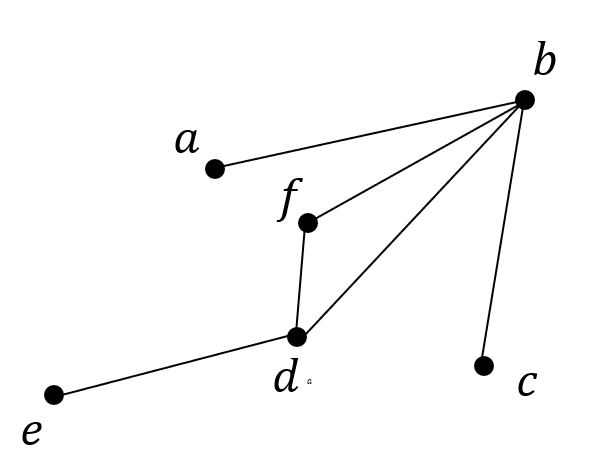
\includegraphics[width=0.6\linewidth]{img/deelgraaf2.jpg}
\captionof{figure}{Een opspannende deelgraaf van $G$}
\label{boom4}
\end{center}

We herhalen de definitie van een boom: een $boom$ is een samenhangende graaf zonder cykels. 

De grafen van figuren \ref{boom1}, \ref{boom2}, \ref{boom3} en \ref{boom4} zijn geen bomen omdat ze een cykel bevatten. In figuur \ref{boom5} zie je een boom. Bovendien is het nog steeds een deelgraaf van de graaf $G$ van figuur \ref{boom1}. De graaf van figuur \ref{boom6}, ook een deelgraaf van $G$, is geen boom omdat die niet samenhangend is. Ten slotte zie je in figuur \ref{boom7} een boom die een opspannende deelgraaf is van $G$, of kortweg een opspannende boom van $G$.

\begin{center}

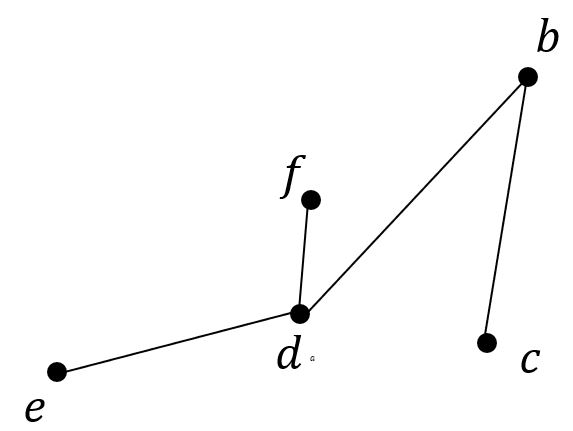
\includegraphics[width=0.6\linewidth]{img/deelgraaf4.jpg}
\captionof{figure}{Een boom}
\label{boom5}
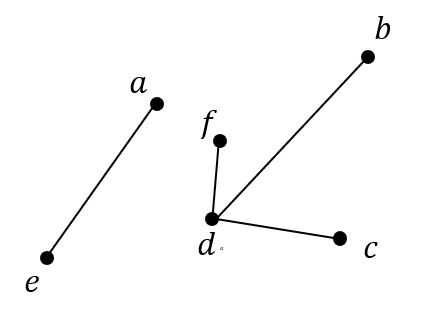
\includegraphics[width=0.6\linewidth]{img/deelgraaf8.JPG}
\captionof{figure}{Geen boom}
\label{boom6}
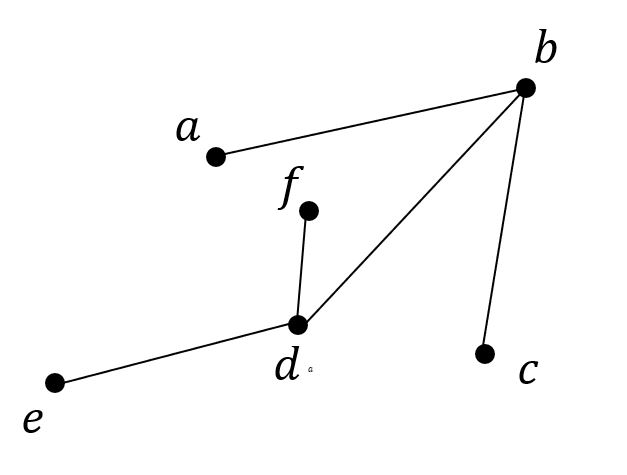
\includegraphics[width=0.6\linewidth]{img/deelgraaf3.jpg}
\captionof{figure}{Een opspannende boom van $G$}
\label{boom7}

\end{center}

Vaak wordt aan de bogen van een graaf een bepaalde getalwaarde toegekend. Bij het aanleggen van een netwerk kan dat de prijs zijn om die verbinding te maken. Bij een wegennetwerk kan dat de afstand zijn van knoop tot knoop via die weg. Maar het kan ook de tijd zijn. Als wij voor een redactievergadering van jullie geliefde tijdschrift van Leuven naar Sinaai rijden, kun je de routeplanner vragen om de kortste route te zoeken, maar je kunt ook vragen om de snelste route te zoeken. De kortste route gaat via Puurs en Temse, maar de snelste gaat via Antwerpen (tenzij er file is op de Antwerpse ring).

Een graaf waarbij er getallen staan bij de bogen, heet een $gewogen$ graaf. Die getallen noemen we de $gewichten$ van de bogen.

Als deze begrippen door de leerlingen gekend zijn, zijn ze klaar voor de volgende werktekst. Hierin wordt gezocht, in gegeven grafen, naar een opspannende deelgraaf die een boom is, kortom een opspannende boom. Bovendien willen we het totale gewicht zo klein mogelijk hebben. We gaan dus op zoek naar een \emph{minimale opspannende boom} van de gegeven gewogen graaf.

We laten de leerlingen zelf een algoritme bedenken en vergelijken met twee beroemde algoritmen met hetzelfde doel: het algoritme van Prim en dat van Kruskal.

\end{multicols}

\beginwerktekst{Algoritmen voor minimale opspannende bomen}

In de gewogen graaf $G$ hieronder zijn de knopen vijf steden. De gewichten van de bogen zijn de (afgeronde) afstanden in km. 
\begin{center}
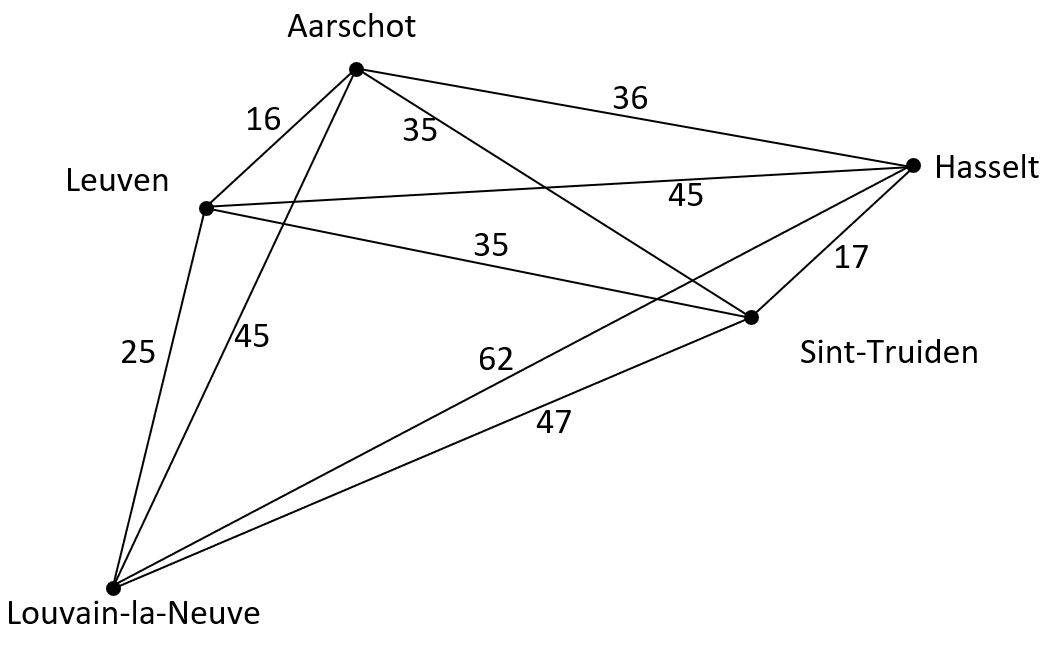
\includegraphics[width=0.70\linewidth]{img/steden.jpg}
\end{center}

Men wil deze vijf steden verbinden met glasvezels. Hieronder zie je een manier: graaf $H$. Het gaat over de graaf met bogen in volle lijnen, de bogen in grijze stippellijn horen er niet bij; het zijn de bogen van $G$ die niet tot $H$ behoren.

\begin{center}
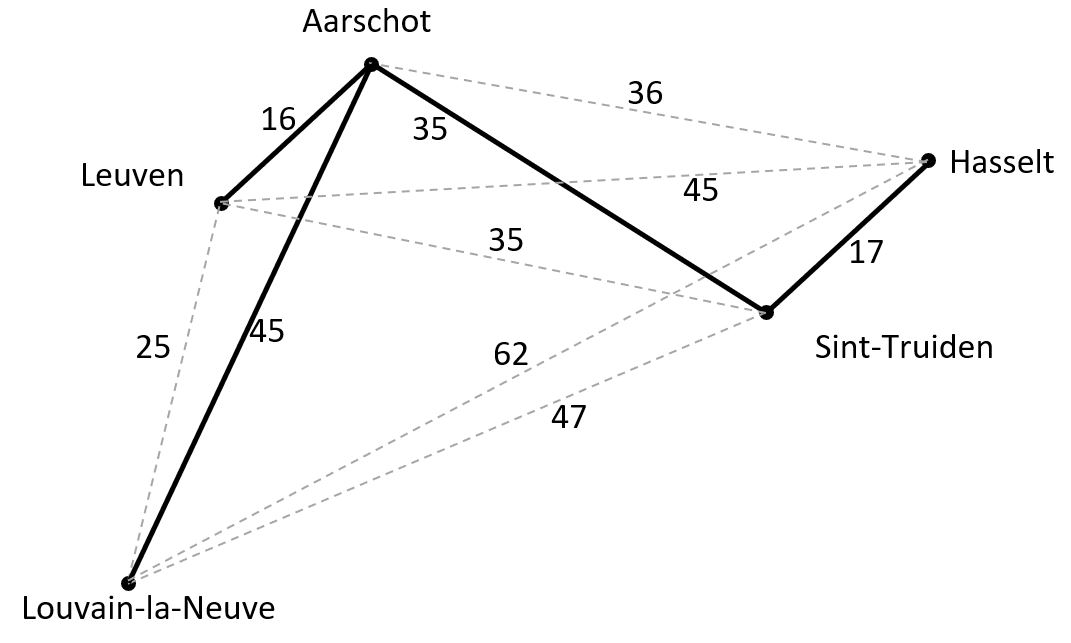
\includegraphics[width=0.70\linewidth]{img/steden2.jpg}
\end{center}

\begin{nummering}

\item Is $H$ een deelgraaf van $G$? Waarom?

\item Is $H$ een opspannende deelgraaf van $G$?

\item Is $H$ een boom? Waarom?

\item Is $H$ de beste manier om de vijf steden te verbinden? Of kan het met minder glasvezel in totaal? Hoe zou jij het doen?

\emph{Het totale gewicht van $H$ is 113. Een opspannende boom met kleiner totaal gewicht zie je hieronder. Hier is het totale gewicht 93. Er is nog een tweede oplossing met totale gewicht 93: wanneer de boog tussen Leuven en Sint-Truiden vervangen wordt door de boog tussen Aarschot en Sint-Truiden.}

\begin{center}
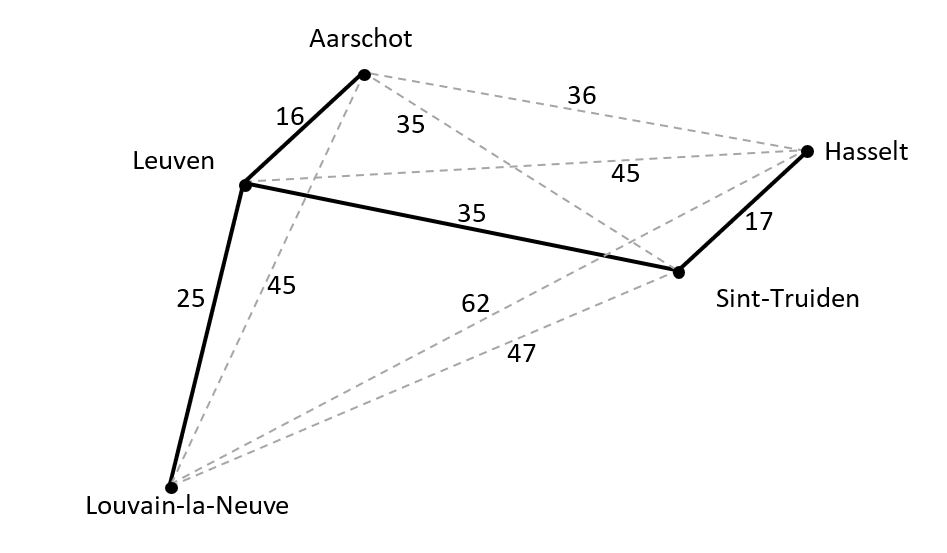
\includegraphics[width=0.70\linewidth]{img/stedenprim4.jpg}
\end{center}

\end{nummering}

Men zoekt vaak een \emph{minimale} opspannende boom voor een graaf. Dit is een opspannende deelgraaf die een boom is en bovendien het kleinst mogelijke totale gewicht heeft.

In de volgende figuur zie je een kaart van de belangrijkste steden van Engeland (uit Belsom e.a., 1994). 

\begin{center}
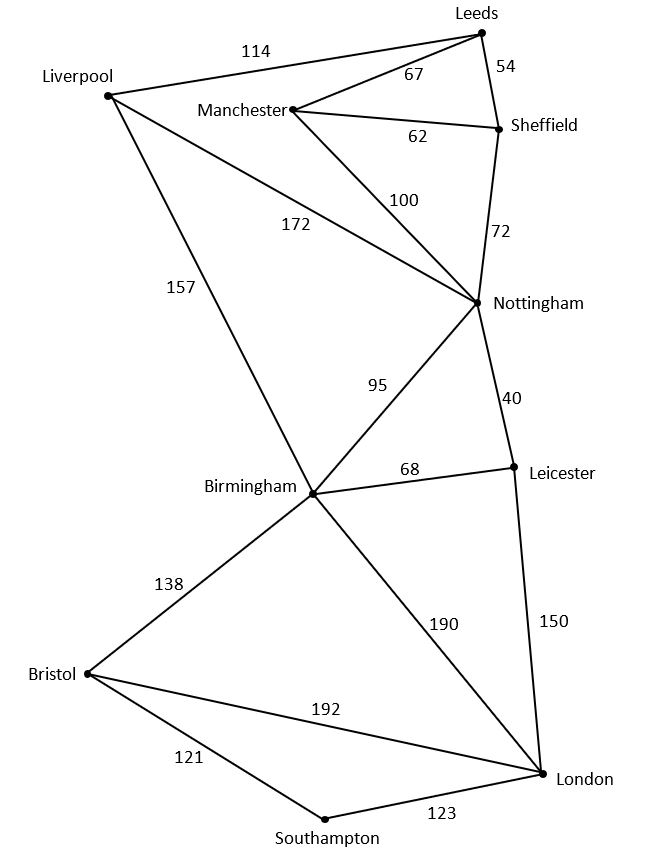
\includegraphics[width=0.75\linewidth]{img/Engelsesteden.JPG}
\end{center}

\begin{nummering}

\setcounter{enumi}{4}


\item Bedenk een systematische methode om een opspannende boom te vinden met een zo klein mogelijk totale gewicht. Formuleer je methode (in het algemeen).

\emph{Het is best mogelijk dat leerlingen zelf een algoritme bedenken dat op hetzelfde neerkomt als het algoritme van Prim of het algoritme van Kruskal (zie hieronder). We vinden het belangrijk om hen de kans te geven om zelf zo'n algoritme te bedenken. De leraar stuurt bij als hun formulering niet duidelijk of niet eenduidig is. Het algoritme moet wel leiden tot een boom (dus: cykels zijn niet toegelaten) en tot een opspannende boom (op het einde moeten alle knopen bereikt worden).}

\item Pas je methode toe op de graaf van de Engelse steden.

\emph{Hier is de oplossing.}

\begin{center}
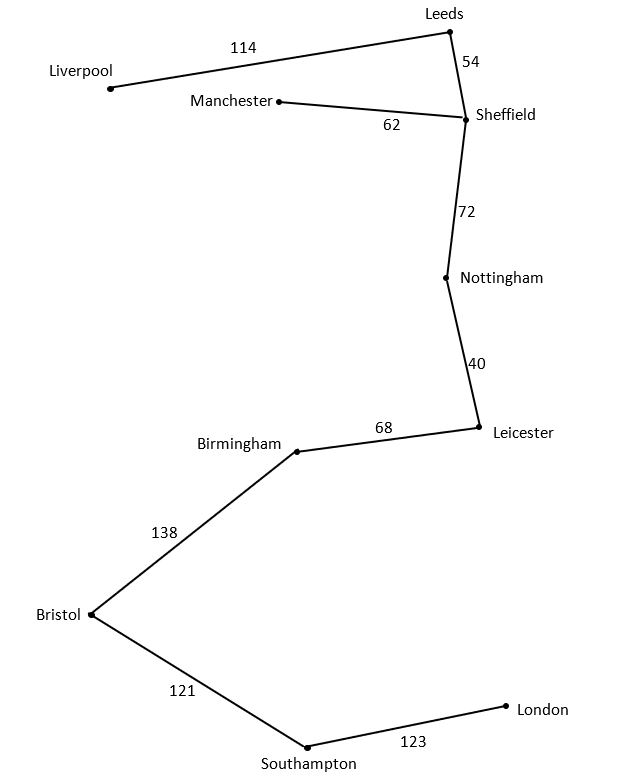
\includegraphics[width=0.60\linewidth]{img/Engelsestedenopl.JPG}
\end{center}



\end{nummering}

Hieronder staan twee beroemde algoritmen om een minimale opspannende boom te bepalen. 

\tussentitel{Algoritme van Prim (Robert C. Prim, Amerikaanse wiskundige en informaticus, 20ste eeuw)}

Gegeven is een gewogen graaf $G$. Stap voor stap bouwen we aan een deelgraaf $H$, die op het einde een minimale opspannende boom van $G$ zal zijn.
\begin{opsomming}
\item Kies een willekeurige knoop van $G$. $H$ is om te beginnen de triviale graaf bestaande uit enkel deze ene knoop.
\item Neem van de bogen van $G$ die $H$ rechtstreeks verbinden met een knoop die nog niet in $H$ zit, die met het kleinste gewicht. (Bij ex aequo mag je kiezen.) Voeg deze boog en deze knoop toe aan $H$.
\item Blijf de vorige stap herhalen tot alle knopen van $G$ in $H$ zitten. 
\end{opsomming}

Hieronder tonen we met het voorbeeld van de Vlaamse steden, de tussenstappen bij het algoritme van Prim, vertrekkend van Aarschot. 




\begin{multicols}{2}
\begin{center}
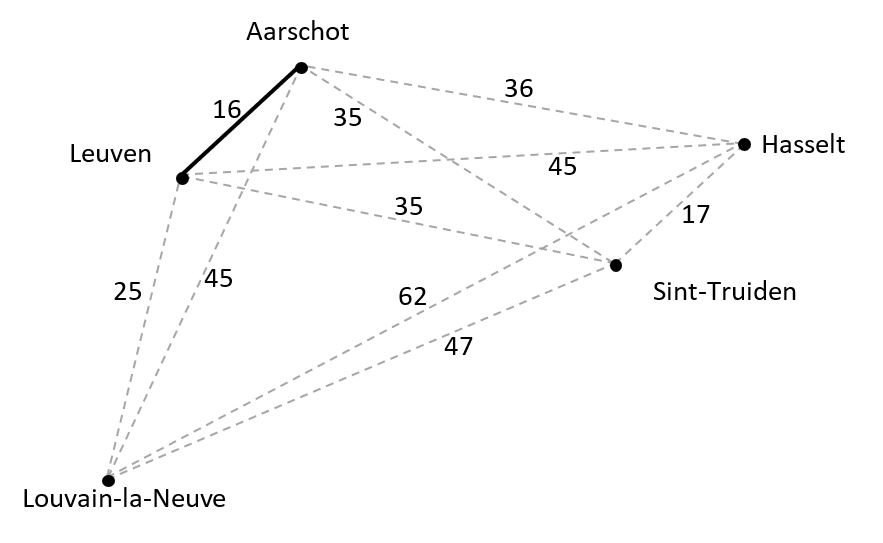
\includegraphics[width=\linewidth]{img/stedenstap1.JPG}

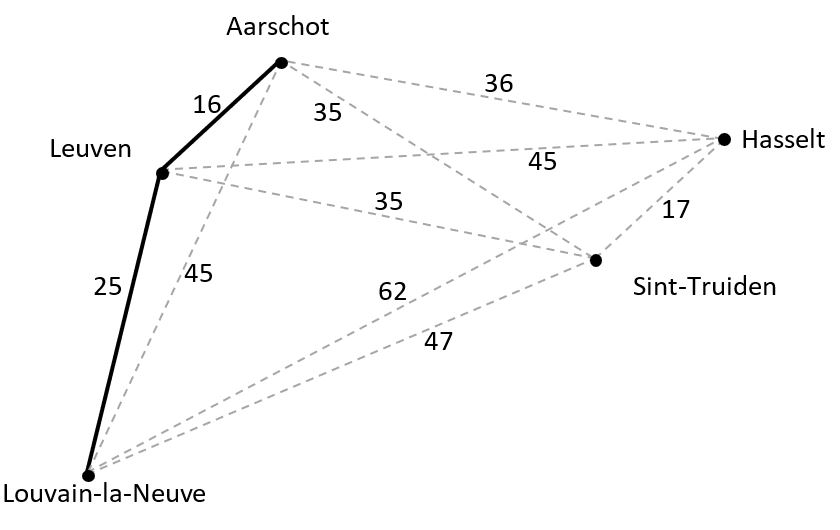
\includegraphics[width=\linewidth]{img/stedenprim2.JPG}

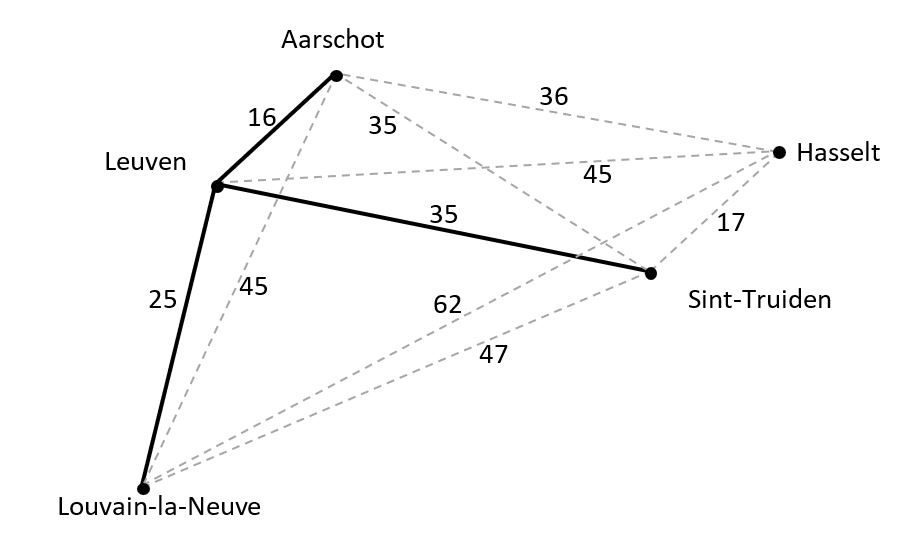
\includegraphics[width=\linewidth]{img/stedenprim3.JPG}

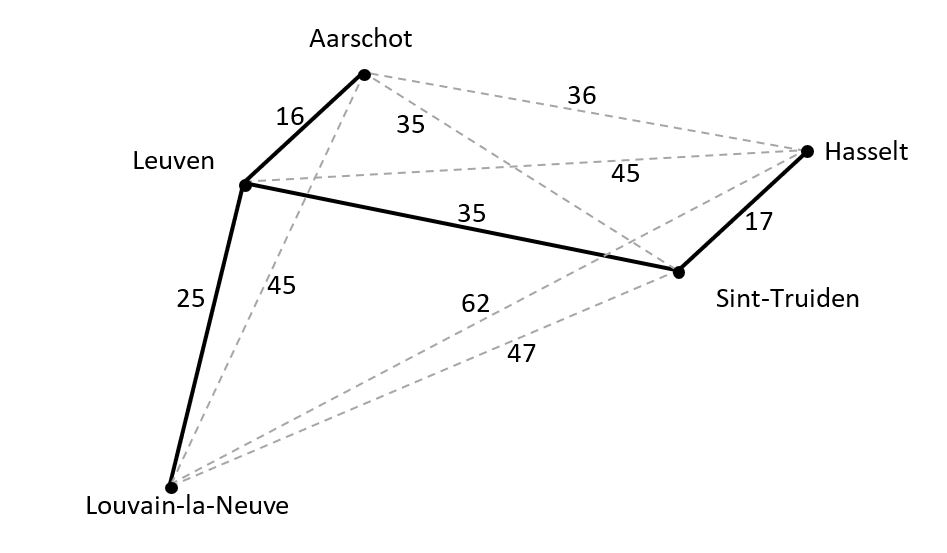
\includegraphics[width=\linewidth]{img/stedenprim4.JPG}
\end{center}

\end{multicols}

\tussentitel{Algoritme van Kruskal (Joseph B. Kruskal, Amerikaanse wiskundige en statisticus, 20ste eeuw)}

Gegeven is een gewogen graaf $G$. Stap voor stap bouwen we aan een deelgraaf $H$, die op het einde een minimale opspannende boom van $G$ zal zijn.
\begin{opsomming}
\item Neem de boog van $G$ die het kleinste gewicht heeft. (Bij ex aequo mag je kiezen.) $H$ bestaat om te beginnen uit deze boog en zijn twee eindknopen.
\item Bepaal de boog van $G$ die nog niet in $H$ zit, geen cykel doet ontstaan in $H$ en het kleinste gewicht heeft. (Bij ex aequo mag je kiezen.) Voeg deze boog en zijn eindknopen toe aan $H$.
\item Blijf de vorige stap herhalen tot alle knopen van $G$ in $H$ zitten. 
\end{opsomming}

Hieronder zie je het algoritme van Kruskal in zijn werk voor de Vlaamse steden.

\begin{multicols}{2}

\begin{center}
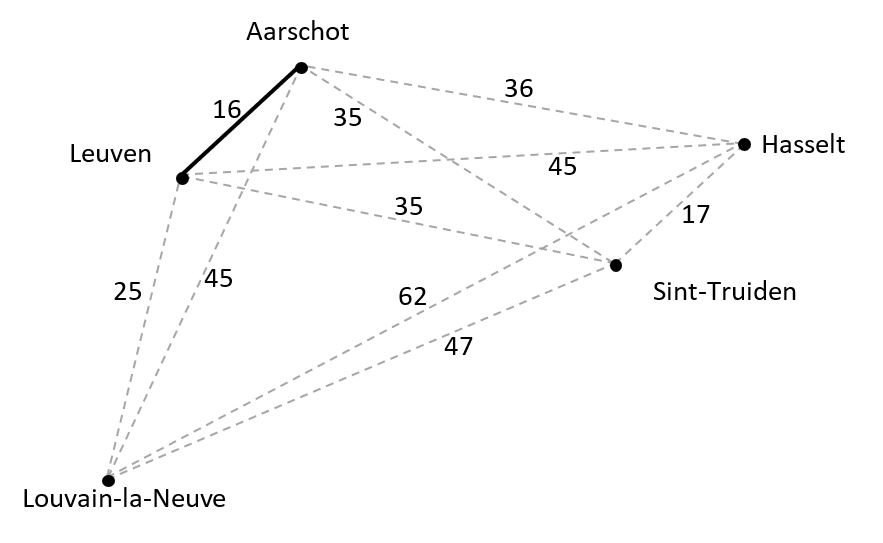
\includegraphics[width=\linewidth]{img/stedenstap1.JPG}

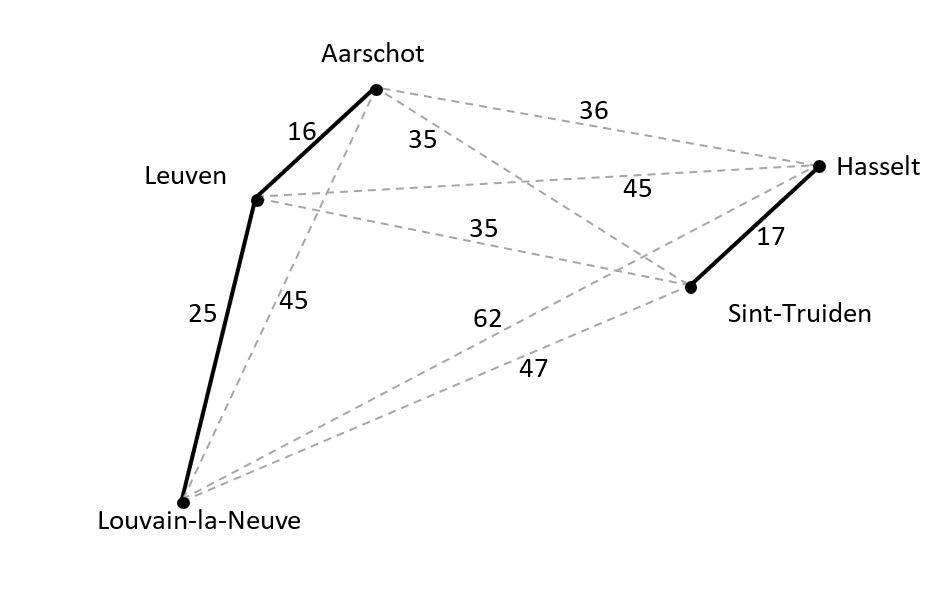
\includegraphics[width=\linewidth]{img/stedenkruskal3.JPG}

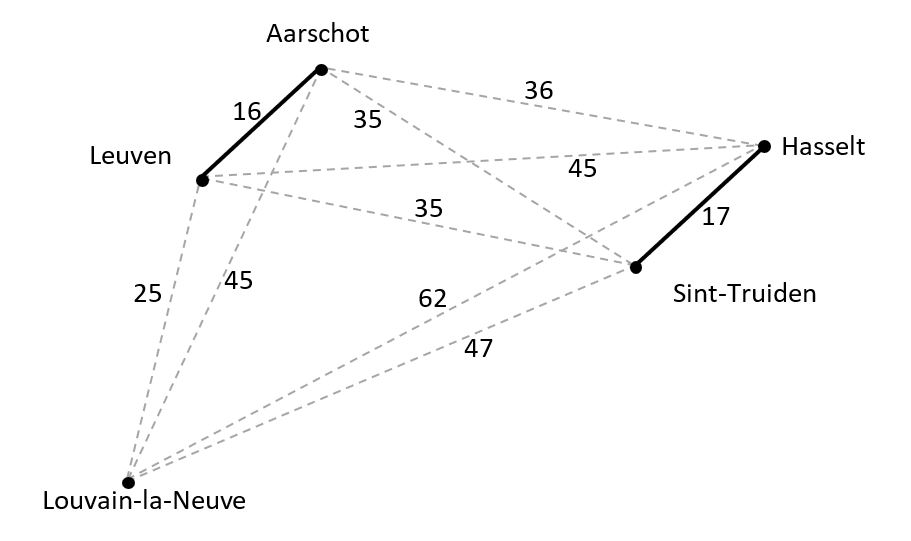
\includegraphics[width=\linewidth]{img/stedenkruskal2.JPG}

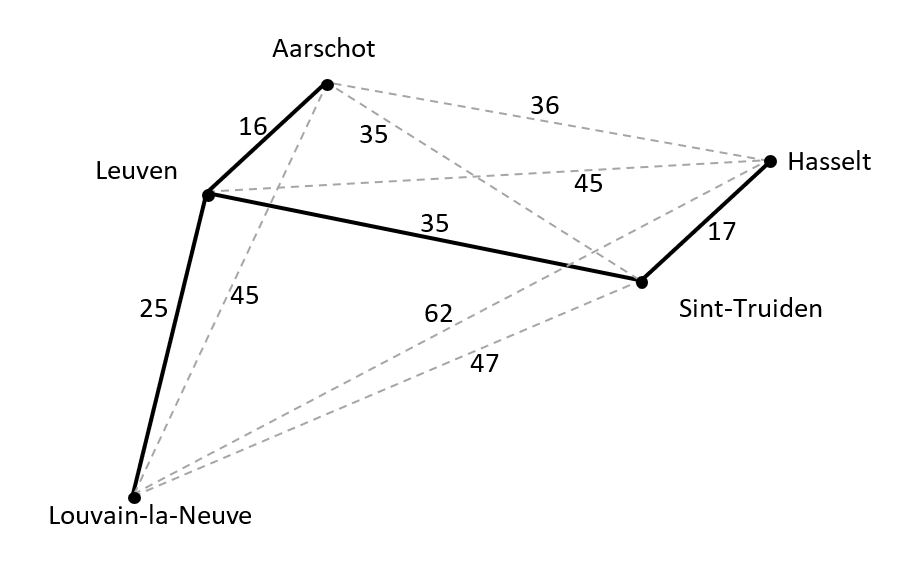
\includegraphics[width=\linewidth]{img/stedenopl.JPG}

\end{center}

\end{multicols}

\begin{nummering}

\setcounter{enumi}{6}

\item Vergelijk jouw methode met de algoritmen van Prim en Kruskal.

\end{nummering}


\eindewerktekst

\begin{multicols}{2}

Merk op: als sommige gewichten gelijk zijn, is de oplossing niet noodzakelijk uniek. Wanneer alle gewichten verschillend zijn, zullen beide algoritmen dezelfde oplossing geven. Bij Prim heb je in elke stap een boom; bij Kruskal heb je in de tussenstappen niet noodzakelijk een samenhangende deelgraaf.

Jammer dat deze algoritmen al bestaan en een naam hebben gekregen, anders zouden leerlingen er beroemd mee kunnen worden...






%\subsection{Typ hier de deelparagraaftitel}
%Typ hier je tekst


%\tussentitel{Typ hier de tussentitel}
%Typ hier je tekst


\end{multicols}


%%% Hieronder enkele speciale omgevingen %%%
%%%%%%%%%%%%%%%%%%%%%%%%%%%%%%%%%%%%%%%%%%%%

% % een figuur invoegen (gecentreerd) op de plaats waar je die typt. Vervang enkel de documentnaam.
% \begin{center}
% \includegraphics[width=\linewidth]{img/loodrecht.jpg}
% \captionof{figure}{Hier typ je het bijschrift}
% \end{center}


 
% % een floatende figuur invoegen (gecentreerd) op de plaats waar het volgens het systeem best is. Vervang enkel de documentnaam. Als het kan: floatende figuur vermijden (dat is makkelijker voor de lay-outers). 
% \begin{figure}[H]
% \begin{center}
% \includegraphics[width=\linewidth]{img/heroon.jpg}
% \captionof{figure}{Hier typ je het bijschrift}
% \end{center}
% \end{figure}


% % een opsomming met bullets:
% \begin{opsomming}                                       % er is ook een opsommingbreed (met meer interlinie)
% \item tekst
% \item tekst
% \end{opsomming}

% % een opsomming met getallen:
% \begin{nummering}                                       % er is ook een nummeringbreed (met meer intelinie)
% \item tekst
% \item tekst
% \end{nummering}

% % een gewone kader rond tekst
% \begin{kader}
% Typ hier je tekst
% \end{kader}



% % een kader met nummering en 3 argumenten: het genummerde onderwerp, de verklaring en de tekst
% \begin{stellingkader}
% {Stelling}{Naam van de stelling of het besluit}{Typ hier de eigenlijke stelling}
% \end{stellingkader}

% % een kader zonder nummering en 3 argumenten: het onderwerp, de verklaring en de tekst
% \begin{stellingkadertwee}
% {Besluit}{Naam van de stelling of het besluit}{Typ hier de eigenlijke stelling}
% \end{stellingkadertwee}

% % een gekleurd kader met nummering en 3 argumenten: het genummerde onderwerp, de verklaring en de tekst
% \begin{kleurkader}
% {Stelling}{Naam van de stelling of het besluit}{Typ hier de eigenlijke stelling}
% \end{kleurkader}

% \begin{multicols} {2}
% \lipsum[6]

% %%% een lesactiviteit invoegen (daarom \end{multicols})
% \end{multicols}
% \beginwerktekst{Typ hier de titel van de lesactiviteit}
% \begin{werktekstoef}
% \item{typ hier de vraag}

% \emph{typ hier het antwoord}

% \item{typ een nieuwe vraag}

% \emph{het antwoord}
% % oefeningomgeving stoppen om tussentekst in te voegen als dat nodig is
% \end{werktekstoef}  

% tussentest\lipsum[1]

% \begin{werktekstoef}
% \setcounter{enumi}{2}                       % om de vorige nummering door te laten lopen
% \item{typ hier de vraag}

% \emph{typ hier het antwoord}

% \item{typ een nieuwe vraag}

% \emph{het antwoord}

% \end{werktekstoef}
% \eindewerktekst


% \stopcontents[mainsections]			        % altijd laten staan, opsomming in inhoudstafel enkel tot loep beperken


% % bronnen toevoegen
\begin{bronnen}

\item Aldous, J., Wilson, R. (2004). \emph{Graphs and applications, an introductory approach.} London, Berlin, Heidelberg: Springer-Verlag.

\item Alsina, C. (2010). \emph{Mapas del metro y redes neuronales. La teoría de grafos.} Barcelona: RBa Libros.

\item Belsom, C. e.a. (1994). \emph{Networks. Student text and unit guide.} Cambridge, New York, Victoria: Cambridge University Press.

\item Benjamin, A., Chartrand, G., Zhang, P. (2015). \emph{The fascinating world of graph theory.} Princeton and Oxford: Princeton University Press. ISBN 978-0-691-17563-8.

\item Bouw, J. (2009). \emph{Doeboek 24/ Grafen.} Leiden: Vierkant voor wiskunde.

\item Broersma, H. (2002). \emph{Grafen in de praktijk}. Zebrareeks nr. 14. Utrecht: Epsilon.

\item Bybyakina, G., Plekhanova, T., Gromova (Shevkoplyas), E., Bubyakina, G. (2017). \emph{Cost Optimization for the Transport Network of Yakutia.} Contributions to Game Theory and Management 10, 7-16. Online beschikbaar via \url{https://www.researchgate.net/publication/318942379_Cost_Optimization_for_the_Transport_Network_of_Yakutia}

\item Chartrand,G. (1977). \emph{Introductory graph theory}. New York: Dover Publications.

\item Curzon, P. (2015). \emph{Computational Thinking: Puzzling Tours.} London: Queen Mary University of London. \url{https://cs4fndownloads.wordpress.com/puzzling-tours/}

\item Fack, V. (2013). \emph{De wiskunde achter een routeplanner.} Unimath 5. Brugge: Die Keure.

\item Perucca, A. (2019). \emph{De zeven bruggen van Koningsbergen}, Uitwiskeling 36/1, 8-10.

\item Wilson, R. (1972, 1996). \emph{Introduction to graph theory}. Harlow: Addison Wesley Longman Ltd., online beschikbaar: \url{ https://www.maths.ed.ac.uk/~v1ranick/papers/wilsongraph.pdf}


\end{bronnen}

